\documentclass[12pt,a4paper,english,twoside]{book}


\usepackage{bera}% optional: just to have a nice mono-spaced font
\usepackage[version=1.6]{listings}
\usepackage{xcolor}
\usepackage{lineno}
\usepackage{caption}
\usepackage{subcaption}
\usepackage{xpatch}


\definecolor{codegreen}{rgb}{0,0.6,0}
\definecolor{codegray}{rgb}{0.5,0.5,0.5}
\definecolor{codepurple}{rgb}{0.58,0,0.82}
\definecolor{backcolour}{rgb}{0.95,0.95,0.92}


\colorlet{punct}{red!60!black}
\definecolor{background}{HTML}{EEEEEE}
\definecolor{delim}{RGB}{20,105,176}
\colorlet{numb}{magenta!60!black}


\lstset{
  frame=top,frame=bottom,
  linewidth=15.4cm,
  numbers=left,
  basicstyle=\small\normalfont\sffamily,    % the size of the fonts that are used for the code
  stepnumber=1,                           % the step between two line-numbers. If it is 1 each line will be numbered
  numbersep=10pt,                         % how far the line-numbers are from the code
  tabsize=2,                              % tab size in blank spaces
  extendedchars=true,                     %
  breaklines=true,                        
  captionpos=t,                          
  stringstyle=\color{white}\ttfamily, % Farbe der String
  showspaces=false,           % Leerzeichen anzeigen ?
  showtabs=false,             % Tabs anzeigen ?
  xleftmargin=20pt,
  framexleftmargin=20pt,
  framexrightmargin=17pt,
  framexbottommargin=5pt,
  framextopmargin=5pt,
  showstringspaces=false,      % Leerzeichen in Strings anzeigen ?
    backgroundcolor=\color{background},
        literate={\ \ }{{\ }}1,
 }

\DeclareCaptionFormat{listing}{\rule{\dimexpr\textwidth\relax}{0.4pt}\par\vskip1pt#1#2#3}
\captionsetup[lstlisting]{format=listing,singlelinecheck=false, margin=0pt, font={sf},labelsep=space,labelfont=bf}

\renewcommand\lstlistingname{Algorithm}


\lstnewenvironment{sflisting}[1][]
  {\lstset{#1}\mathversion{sans}}{}



%\lstdefinelanguage{json}{
  
%}

%breaklines=true,                 
 %   tabsize=2,literate={\ \ }{{\ }}1,caption={The code block for changing the IP address on the server side from the executeMTDMechanisms() function in pseudocode. Everything related to the port change was ommited here.},captionpos=b,label={lst:Pseudocode sendToDevicesIP.py}, frame=tb]


\lstdefinestyle{mystyle}{    backgroundcolor=\color{backcolour},   commentstyle=\color{codegreen},
    keywordstyle=\color{magenta},
    numberstyle=\tiny\color{codegray},
    stringstyle=\color{codepurple},
    basicstyle=\ttfamily\footnotesize,
    breakatwhitespace=false,         
    breaklines=true,                 
    captionpos=b,                    
    keepspaces=true,                 
    numbers=left,                    
    numbersep=5pt,                  
    showspaces=false,                
    showstringspaces=false,
    showtabs=false,                  
    tabsize=2
}



\usepackage[german,english]{babel}
\usepackage[T1]{fontenc} 
\usepackage[utf8]{inputenc}
\usepackage{amsfonts}
\usepackage{amsmath}
\usepackage{latexsym}
\usepackage{amssymb}
\usepackage{epsfig}
\usepackage{moreverb}
\usepackage{rotating}
\usepackage{enumerate}
\usepackage{graphics, graphicx,wrapfig}
\usepackage{fancybox}
\usepackage{picinpar,varioref,floatflt}
\usepackage{ae}
\usepackage{longtable}
\usepackage{textcomp}
\usepackage{float}
\usepackage[acronym]{glossaries}
\usepackage{todonotes}
\usepackage{algorithm}
\usepackage{algpseudocode}
\usepackage[obeyspaces]{url}
\usepackage{lscape}
\PassOptionsToPackage{hyphens}{url}\usepackage{hyperref}
\usepackage[
style=ieee,
]{biblatex}
%\usepackage{assets/unizhdt-BA} %Bachelor Thesis
\usepackage{assets/unizhdt-MA} %Master Thesis   



\addbibresource{assets/refs.bib}

%%%%%%%%%%%%%%%%%%%%%%%%%%%%%%%%%%%%%%%%%%%%%%%%%%
\newcommand{\etal}{\textit{et al}.\ }
\newcommand{\ie}{\textit{i}.\textit{e}.,\ }
\newcommand{\eg}{\textit{e}.\textit{g}.,\ }
\newcommand{\cf}{\textit{c}\textit{f}.,\ }
%%%%%%%%%%%%%%%%%%%%%%%%%%%%%%%%%%%%%%%%%%%%%%%%%%


% Define the language of the diploma thesis
\selectlanguage{english}
%\selectlanguage{german}

\pagestyle{headings}
\newacronym{mtd}{MTD}{Moving Target Defense}

\renewcommand\linenumberfont{\scriptsize}


\xpatchbibdriver{online}
  {\printtext[parens]{\usebibmacro{date}}}
  {\iffieldundef{year}
    {}
    {\printtext[parens]{\usebibmacro{date}}}}
  {}
  {\typeout{There was an error patching biblatex-ieee (specifically, ieee.bbx's @online driver)}}

\usepackage{xurl}


\begin{document}

%%%%%%%%%%%%%%%%%%%%%%%%%%%%%%%%%%%%%%%%%%%%%%%%%%

% Define the author printed on the cover page
\author{Steven Näf}
% Define the city and country of the author
\authorcity{Zurich, Switzerland}
% Define the student ID (Matrikelnummer)
\studentid{15-710-254}
% Define the title with optional subtitle
\title{Design and Implementation of a Cooperative MTD Framework for 
IoT Devices}
% Define the supervisors
\supervisors{Jan von der Assen, Dr. Alberto Huertas Celdrán}
% Define the submission date
\submissiondate{January 29, 2023}

%%%%%%%%%%%%%%%%%%%%%%%%%%%%%%%%%%%%%%%%%%%%%%%%%%

% Make the title page
\maketitle

% Make the imprint on the back of the cover page
\makeimprint

\pagenumbering{roman}

% Include the files of the diploma thesis
%\cleardoublepage
\chapter*{Abstract}
\addcontentsline{toc}{chapter}{Abstract}


\selectlanguage{english} 
The Internet of Things (IoT) offers many advantages to our society, including benefits regarding the economy and human convenience. While these are not empty promises, IoT devices have the major drawback of being inherently vulnerable to malware due to various characteristics. As the number of IoT devices is expected to triple by 2030, possible defense mechanisms against such malware (e.g. Bashlite or Mirai) are essential. This thesis proposed and implemented a prototype of a cooperative and reactive Moving Target Defense (MTD) framework that exploits the weaknesses of Bashlite, a well-known IoT malware. The first weakness is the ability to disrupt the connection of a Bashlite client from the Bashlite server by changing the client's IP address. The second vulnerability is that Bashlite scans and distributes itself via the Telnet port 23. Hence, the infected device is instructed to change its local IP address to disconnect itself from the Bashlite server, and the other devices in the network are instructed to temporarily move their Telnet service port to hide until Bashlite is rendered harmless. 

Three different evaluation scenarios were created, all consisting of two virtual machines, one of which is infected with Bashlite that attempts to infect the second machine. The scenarios differed in the inclusion of the cooperative component and the trigger of the execution of the MTD techniques. The two possibilities for the trigger were proactive (every minute) and reactive (after the detection of Bashlite). The evaluation scenarios have shown that the proposed cooperative and reactive framework and techniques have significant advantages over a non-cooperative and reactive approach and a cooperative but proactive approach. In addition to halving the overall infection time in the system, the overall availability of the machines, defined by outgoing packet losses and outgoing and incoming Telnet connections, was also significantly improved. In addition, the CPU and RAM usage of the framework and techniques executed were minimal. Although the cooperative and reactive approach provided by far the best results, each MTD approach has its advantages and further research is required to make use of this promising defense mechanism.

\clearpage
\selectlanguage{german}
Das Internet der Dinge (Internet of Things, IoT) bringt unserer Gesellschaft viele Vorteile, unter anderem im Bereich der Wirtschaft und des menschlichen Komforts. Das sind zwar keine leeren Versprechungen, allerdings haben IoT Geräte den grossen Nachteil, dass sie aufgrund verschiedener Eigenschaften stark anfällig für Schadsoftware sind. Da sich zusätzlich die Zahl der IoT-Geräte bis 2030 voraussichtlich verdreifachen wird, sind mögliche Abwehrmechanismen gegen solche Schadsoftware (z. B. Bashlite oder Mirai) von entscheidender Bedeutung. In dieser Thesis wurde ein Prototyp eines Frameworks für ein kooperatives und reaktives Verteidigungssystem (Moving Target Defense, MTD) vorgeschlagen und implementiert. Dieser Verteidigungsmechanismus nutzt die Schwachstellen von Bashlite, einer bekannten IoT Malware, aus. Die erste Schwachstelle ist die Möglichkeit, die Verbindung eines Bashlite-Clients mit dem Bashlite-Server zu unterbrechen, indem die IP-Adresse des Clients geändert wird. Die zweite Schwachstelle besteht darin, dass Bashlite den Telnet-Port 23 von anderen Maschinen scannt und sich darüber auch verbreitet. Wegen diesen zwei Schwachstellen wird die infizierte Maschine angewiesen, die lokale IP-Adresse zu ändern, um sich vom Bashlite-Server zu trennen, und die anderen Geräte im Netzwerk werden angewiesen, ihren Telnet-Service-Port vorübergehend auf einen anderen Port zu legen, bis Bashlite unschädlich gemacht ist.

Drei unterschiedliche Bewertungsszenarien wurden erstellt, wobei alle aus zwei virtuellen Maschinen bestehen, von denen eine mit Bashlite infiziert ist, die dann versucht die zweite Maschine zu infizieren. Die Szenarien unterschieden sich durch die Einbeziehung der kooperativen Komponente und durch den Auslöser für die Ausführung der MTD-Techniken. Die beiden Möglichkeiten für den Auslöser waren proaktiv (jede Minute) und reaktiv (nach der Erkennung von Bashlite). Diese Bewertungsszenarien haben gezeigt, dass das vorgeschlagene Framework und die Techniken (kooperativ und reaktiv) erhebliche Vorteile gegenüber einem unkooperativen und reaktiven Ansatz und einem kooperativen, aber proaktiven Ansatz haben. Neben der Halbierung der Gesamtinfektionszeit im System wurde auch die Verfügbarkeit der Maschinen, definiert durch ausgehende Paketverluste und ausgehende und eingehende Telnet-Verbindungen, insgesamt deutlich verbessert. Darüber hinaus war die CPU- und RAM-Auslastung des Frameworks und der ausgeführten Techniken minimal. Obwohl der kooperative und reaktive Ansatz bei weitem die besten Ergebnisse lieferte, hat jeder MTD-Ansatz seine Vorteile, und weitere Forschung ist erforderlich, um diesen vielversprechenden Abwehrmechanismus entsprechend zu nutzen.


\selectlanguage{english} 






%\cleardoublepage
\chapter*{Acknowledgments}
\addcontentsline{toc}{chapter}{Acknowledgments}

I would like to thank my two supervisors, Jan von der Assen and Dr. Alberto Huertas Celdrán. They have helped me with all kinds of problems, given much appreciated input when it was not clear how to proceed, and provided great feedback overall. All of this has contributed greatly to the quality of this thesis and also helped me going through the more difficult times while writing the thesis. 

\tableofcontents

\cleardoublepage
\pagenumbering{arabic}
\chapter{Introduction}



\section{Motivation}
In today's world, IoT devices are already ubiquitous and can be found in several major end-use industries such as healthcare, manufacturing or banking~\cite{website:fortuneIoT}. In 2021, there were 11.3 billion IoT devices worldwide and this number is expected to triple by 2030~\cite{website:statistaIoT}. These devices facilitate the integration of the physical world into a computer-based system, providing various benefits such as improved efficiency and economic advantages~\cite{report:cern}. However, alongside the many benefits, there are also major security concerns, as the devices are popular targets for malware for a number of reasons. These include poor maintenance by manufacturers and weak/repetitive device passwords~\cite{article:DDoSinIoT,website:IBMIoT}. Infected IoT devices are ideal as bots for botnets, which can then launch e.g. distributed denial of service attacks. \cite{website:KasperskyAMalwareStory}~detected 105 million attacks on its honeypots in the first half of 2019, which is a significant increase from the 12 million attacks registered in the first half of 2018. The security problems, the rapidly growing number of devices worldwide and the increasing number of attacks make a strong defence option indispensable.  

One possible defence solution is Moving Target Defence (MTD). This is a cybersecurity paradigm that was first proposed in 2009~\cite{navas:2021MTDWhere}. Its aim is to constantly change the attack surface of a target to diminish the probability of a successful attack~\cite{navas:2021MTDWhere}. Examples include dynamic network techniques, which change network properties such as a device's IP address, or dynamic data techniques, which aim to change data representations~\cite{article:okhraviFindingFocus}. 

IoT malware such as Mirai or Bashlite include a spreading functionality~\cite{article:evOfBashlite}. This allows the malware to quickly spread to new devices, which in turn increases the power of the botnet at hand. This thesis aims to take this spreading functionality into account and create a cooperative MTD framework that mitigates/prevents the malware in a more effective way than a non-cooperative MTD framework is capable of.

\section{Description of Work}
This thesis proposes, implements and evaluates a cooperative MTD framework with two different MTD techniques. The framework is based on~\cite{article:Cedeno}, but includes a cooperative component to mitigate the selected malware and prevent its spreading. The selected malware is Bashlite, a well-known command and control malware, which was modified and completed for this thesis. After analyzing the weaknesses of Bashlite for possible levers where MTD techniques can be applied, two MTD techniques are selected and implemented. The first is to change the IP address of the infected device, which permanently disrupts communication with the Bashlite control server. The second technique is to temporarily change the Telnet service port of other susceptible machines in the network. As many IoT malware infect other devices via the Telnet port, temporarily moving the Telnet service port of the susceptible devices prevents the devices from being found in the first place. After a specified number of seconds, when the IP address change has finished securing the infected device, the Telnet service port changes back to port 23.

The framework and techniques are evaluated in three different scenarios using three different metrics. These metrics include the overall infection time of the system, the interruption of the availability of the machines and the CPU and RAM usage needed by the MTD framework and its techniques. The base case for the evaluation is a non-cooperative and reactive MTD framework that only uses the IP address change to clear the devices after Bashlite is found on them. Reactive means that there is a detection mechanism for the malware and the MTD techniques start as soon as the malware is found on the system. So in the first scenario, each machine has to be infected before it can do anything against Bashlite. The second scenario is cooperative and reactive. As soon as Bashlite is found on a machine on the network, the infected machine initiates the IP address change and all other machines in a given IP range change their Telnet service port to a different port. This is the solution presented in this thesis. The third scenario is cooperative, but proactive. Proactive means that the MTD techniques are run at a specified interval, in this case 60 seconds. Following the evaluation, its results are presented and discussed in-depth. 


\section{Thesis Outline}
After this introductory chapter, the thesis continues with the necessary background information (Chapter 2) for the rest of this thesis. Various information is presented there, including a general overview of MTD and why IoT devices are susceptible to malware. This chapter is followed by the related research chapter (Chapter 3), which first presents the state of research of MTD in IoT, then introduces some MTD IoT frameworks, and finally introduces some MTD IoT mechanisms/techniques. Chapter 4 is the implementation chapter, which deals with the selection and adaptation of Bashlite and possible levers where MTD techniques could be applied to mitigate a Bashlite infection. Additionally, the final implementation is presented in detail in the implementation chapter. This final implementation is then evaluated in Chapter 5, which first introduces the methodology of the evaluation and then presents the results. The last two chapters of the thesis are the discussion and the conclusion. Additionally, some limitations are presented in the discussion and possible future research in the conclusion. 



\chapter{Background} \label{section:background}
This chapter provides an overview of the background knowledge relevant for the thesis. First, a general overview of Moving Target Defence (\acrshort{mtd}) is introduced. Second, some background information on IoT security is presented. This includes some architectural information as well as common IoT malware and how they work. A subsection on cooperative defence concludes the chapter.

\section{General Overview of Moving Target Defense} \label{section:MTD}
Although the idea of modifying system components to prevent others from disrupting the systems has been around for some time, the first use of the term "MTD" was proposed in 2009 by Networking and Information Technology Research and Development (NITRD)~\cite{navas:2021MTDWhere}. The following paragraph is based on this very NITRD source~\cite{report:GhoshMovingTargetDefense}, which despite its age serves as a good overview of MTD.  

One of the main problems of systems is their relatively static configuration. This static design stems from the fact that, in the past, system requirements focused on simplicity and elegance rather than security, as exploitation of vulnerabilities was not a concern. An example are IP addresses and other configuration parameters that remain static over a relatively long period of time. An adversary needs to know the vulnerabilities of a system in order to attack it effectively. The longer the vulnerabilities exist, the more likely they are to be exploited. Therefore, a static system is a significant advantage for an adversary because it gives them enough time to prepare and plan their attack. This is the motivation behind MTD, which involves building systems that change rapidly to minimise the likelihood of a successful attack. 
%A key challenge for MTD is to ensure that the system remains maintainable and reliable for its users. There is no point in having a secure system if it is not usable and reliable. 

Another great and more recent summary was given by~\cite{navas:2021MTDWhere}. Since system information does not expire, an attacker with enough resources (e.g. time) will ultimately find a vulnerability and succeed in his attack. MTD tries to increase the resources needed for an attacker to succeed by continuously altering the attack surface of the system. The sum of a system's vulnerabilities can be defined as its attack surface~\cite{website:IBMAttack}. 



\cite{article:Cai} concluded from the existing literature that three elements must be defined for an MTD technique to achieve the defence objective. 
\begin{enumerate}
    \item \textbf{What to move}: This defines the moving parameter (MP), which is an essential attribute (e.g. IP address or service port) of an attack target. Each MP has a domain from which its values can be selected. 
    \item \textbf{How to move}: This describes how the MP should be moved. This involves selecting a new MP value from its range and replacing the old MP value. There are several ways to choose the new value, such as randomly, game theoretically or situationally.   
    \item \textbf{When to move}: This describes the frequency with which the current value of the MP should be replaced by the new one. This is a critical element because if the MP changes too often, it could lead to poor system performance; if it changes too little, an attacker could be successful.~\cite{navas:2021MTDWhere} identified three different decision processes in the literature: time-based, event-based and hybrid.
\end{enumerate}


\cite{article:okhraviFindingFocus} reviewed five dominant domains of MTD techniques, including the advantages and disadvantages of each. Below is a presentation of these 5 domains. For each domain,~\cite{article:okhraviFindingFocus} also indicated the phase of the attack that the domain seeks to disrupt. For this, the authors chose a five-phase attack consisting of the following phases: 
\begin{itemize}
    \item Reconnaissance: This phase is mainly limited to observation, where the attacker tries to find a target and collect basic information about it. An example of this is finding the IP address of a host through IP scanning.
    \item Access: In this phase, the adversaries collect detailed information about their target. In the case of e.g. a web server, this could include its operating system or configuration. 
    \item Development: In this phase, the adversaries develop an attack that targets a previously found vulnerability. This can be achieved offline without any connection to the target. 
    \item Launch: In this phase, the adversaries compromise the target by delivering the attack payload. This can be done in a variety of ways, including infected media or over the network.
    \item Persistence: If the adversaries wish to remain in the compromised system, they can install additional entry points into the system, such as backdoors. 
\end{itemize}

Each of the MTD domains described below attempts to disrupt one or more of these phases. This is only an overview of the domains and does not cover specific techniques~\cite{article:okhraviFindingFocus}.     

\subsection{Dynamic Networks}
MTD techniques in this domain modify network properties to increase the required workload for an attacker and thus reduce the probability of a successful attack. These techniques are primarily used to prevent the success of the reconnaissance phase, but can also be used to prevent a successful launch phase. Possible means to achieve these network modifications include frequent address and port changes, or changing the logical network topology. The logical network topology is how devices are arranged in a computer network and how they communicate with each other~\cite{article:Santra2013}. 

One problem with such techniques is that they may hinder convenient use of the system when applied to a service of a system that needs to remain in a known network location. An example are public servers, where such a technique would defeat its purpose as the server would be hidden even for legitimate users. Another challenge is that the degree of uncertainty created for attackers is critical to the effectiveness of randomization. Entropy, a value that depends on the number of possible values and their corresponding probabilities, can measure the uncertainty in a random value, but this entropy is limited in many dynamic network techniques. One reason for this is that IP addresses and port numbers can be limited by the network infrastructure.  


\subsection{Dynamic Platforms}
MTD techniques in this domain focus on modifying the computing platform characteristics. The goal is the disruption of attacks that depend on specific platform properties. There are several properties that can be changed, such as the operating system, storage systems, virtual machine instances, or communication channels. It is possible for the same application to run in parallel in different architectural contexts, or for applications to migrate from machine to machine. In terms of attack phases, these techniques provide protection in all five phases, but are most beneficial in the access, development and persistence phases. This is because an attack is much more difficult if it requires exploits for multiple platforms to succeed. This is especially true if the program is executed in parallel on several instances. 

A problem with dynamic platforms is that these techniques also increase the attack surface because additional code is used to control and manage migrations. Additionally, an attacker may gain an advantage due to a specific vulnerability in the platform on which the application is currently running.   
Another problem with dynamic platforms is that it can be difficult to maintain or synchronise state across platforms in a platform-independent format if required by the application. Even if the state transfer can be performed, care must be taken to ensure that the attacker does not remain in the state, resulting in persistence of the attacker in the system.  


\subsection{Dynamic Runtime Environment}
The goal of dynamic runtime environment techniques is to prevent the exploitation of software vulnerabilities by randomizing the environment in which the application runs. These techniques assume that the attacker already has an exploitable vector, and the techniques are designed to prevent the attack from being executed. One problem that these techniques can prevent is buffer overflow exploits, which can lead to code injection. 
These techniques can be further divided into two sub-domains: Instruction Set Randomization (ISR) and Address Space Randomization (ASR). ISR can take place in the application, the operating system, or the hardware, and its goal is to prevent attackers from predicting how the program will execute. This is done by randomizing the instructions in an application. A specific example of ISR is encrypting instructions at load time and decrypting them just before execution. ASR techniques aim to create a randomized memory layout from a deterministic one. This prevents the possibility of using a known memory address for things like control flow redirection. One of the best known and most widely used runtime techniques is address space layout randomisation (ASLR), which falls into the ASR subdomain. 

Both subdomains have weaknesses, in the case of the ASR subdomain, or more specifically ASLR techniques, it is the fact that typically only a part of the memory of the application is randomized, while the other part remains static. This static part may be sufficient for an attacker to develop a meaningful payload. Another related problem is that only the base address of the memory segment is randomized, but the relative addresses remain unchanged. This means that the attacker can bypass ASLR by using relative addresses. In addition, due to the architectural limitations of the defended system, the randomized memory spaces are often too small, making them vulnerable to brute-force attacks. Regarding ISR, the main weakness is the performance overhead caused by the fact that ISR techniques often rely on software emulations, as there is often no hardware support. There are ISR techniques that depend on low overhead methods as e.g. XOR encryption, but these techniques are weak encryption methods and there is a possibility that the attacker can recover the key to inject correctly encrypted instructions. 


\subsection{Dynamic Software}
The goal of MTD techniques in this domain is to diversify the application without changing its functionality. Equivalent program instructions substitute each other, changing various properties such as the internal data structure layout or the sequence of instructions. This reduces the likelihood of a successful attack, as the attacker must correctly guess the software variant being used. These techniques aim to disrupt the attacks' development and launch phase by creating uncertainty and making code injection and code reuse more difficult. There are several ways to apply these techniques, either by using an application that has its own internal randomization capability, or by creating multiple semantically equivalent binaries.

In practice, there was no widespread use of dynamic software techniques in 2014. The examples that did exist were mostly limited to academic and research environments. Unfortunately, no more recent source on the current situation of dynamic software techniques could be found. There are also several weaknesses of these techniques, one of which is that it is complex to ensure that the diversified application provides the same functionality as the original. There is also a lack of scalability, the possibility of unexpected side effects, and the significant performance overhead associated with heavy binary translation and emulation. Finally, many applications are designed for maximum performance, and semantically equivalent applications could reduce this performance.  


\subsection{Dynamic Data}
The goal of the dynamic data domain is to change the internal or external data representation by changing the properties of the data representation, such as syntax or format. Similar to the dynamic software domain, the semantic context should remain unchanged, but the change in data representation should prevent unauthorized use or access to the content. These techniques should also complicate the development and deployment phases of the attack, as attack development is hampered by the need to find an adequate payload for the various data representations. Some of these techniques have their origins in techniques developed against data corruption. One example is a technique where computations are performed on multiple data representations, providing the ability to detect corrupted or malicious input. Figure \ref{fig:differentDataFormats} shows two different data representations with the same semantics. 

These techniques also have weaknesses. One is that most standard binary formats support only one canonical representation, resulting in a lack of diversity in possible data encodings. Another drawback from a practical point of view is that dynamic data techniques increase the effort required for application development as well as runtime performance, since multiple data representations may have to be processed and monitored.




\begin{figure}[tph]
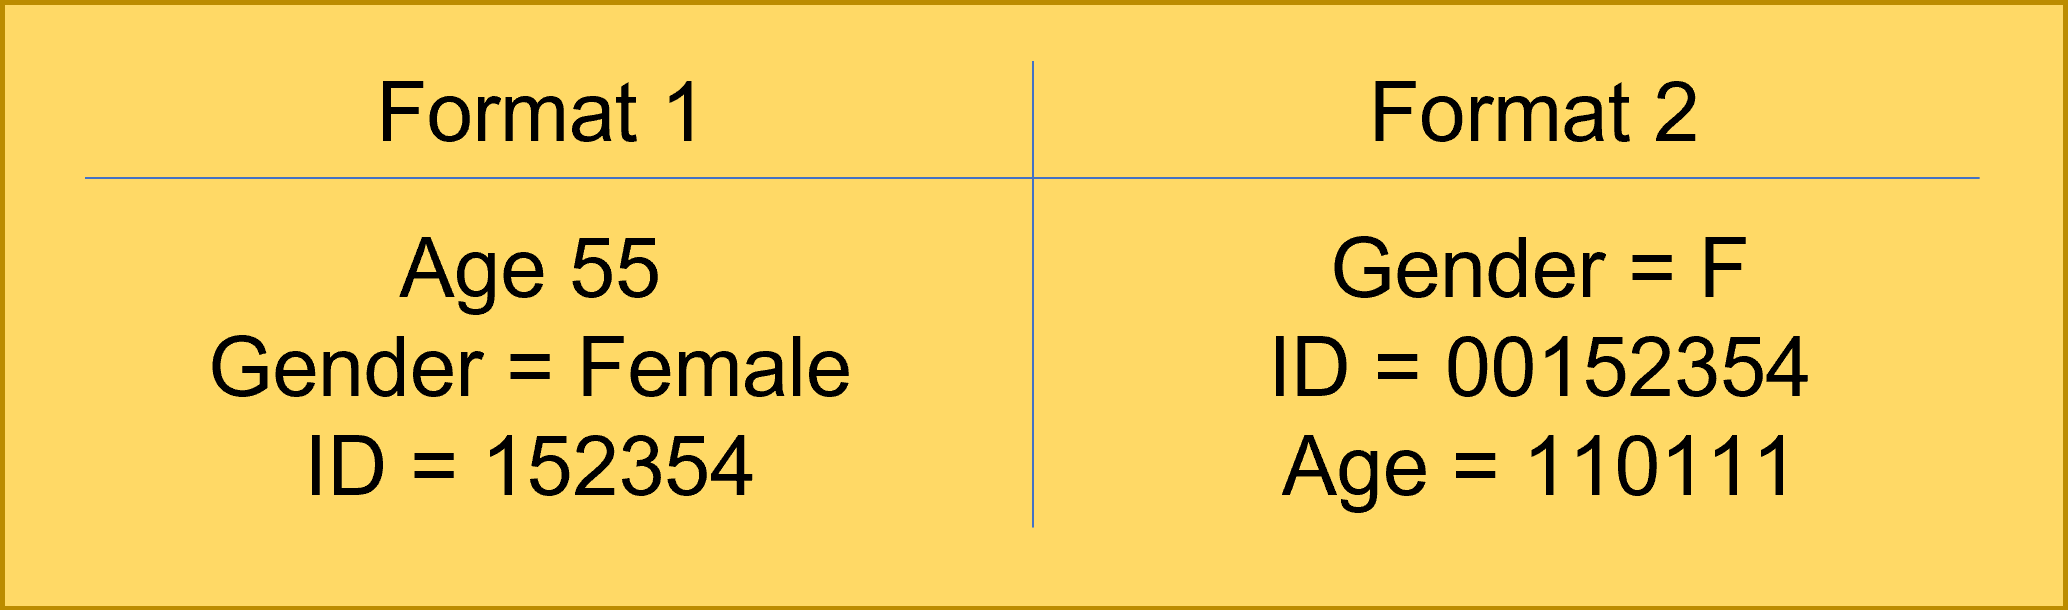
\includegraphics[scale=0.2]{assets/dynamicData.png}
\centering
\caption{Two Different Data Representations With the Same Semantics.}\label{fig:differentDataFormats}
\end{figure}


\subsection{Summary}
Table \ref{table:movingTargetDefense} shows the different moving target defence domains and the corresponding attack phase they seek to disrupt. In their discussion,~\cite{article:okhraviFindingFocus} identified three critical properties for effective MTD, namely unpredictability, comprehensiveness and timeliness. The first property is crucial because if the attacker can predict the next movement of a defence mechanism, the defence becomes obsolete. Comprehensiveness means the inclusion of all elements that could work against an attack, as one element alone may not be very useful. An example is the case where the location of an application's library is randomized, but the application remains in a fixed location. This means that attackers can simply ignore the randomization and attack the fixed code. Timeliness is also important. For example, if attackers can observe the outcome of a moving target defence technique, this knowledge could give them an opportunity to attack. It is also crucial that the attacker is exposed to the diversity of the environment within the attack time. The authors gave an example where an application is migrated among three platforms, so that the attackers would need another vulnerability to continue the attack after the migration to the new platform. However, if the attack time is smaller than the migration time, the security is reduced because the attackers have three different platforms from which to choose vulnerabilities. The authors conclude that some techniques work better for general-purpose environments and some better for specific purposes, as each technique has different strengths and weaknesses.    



\begin{table}[tph]
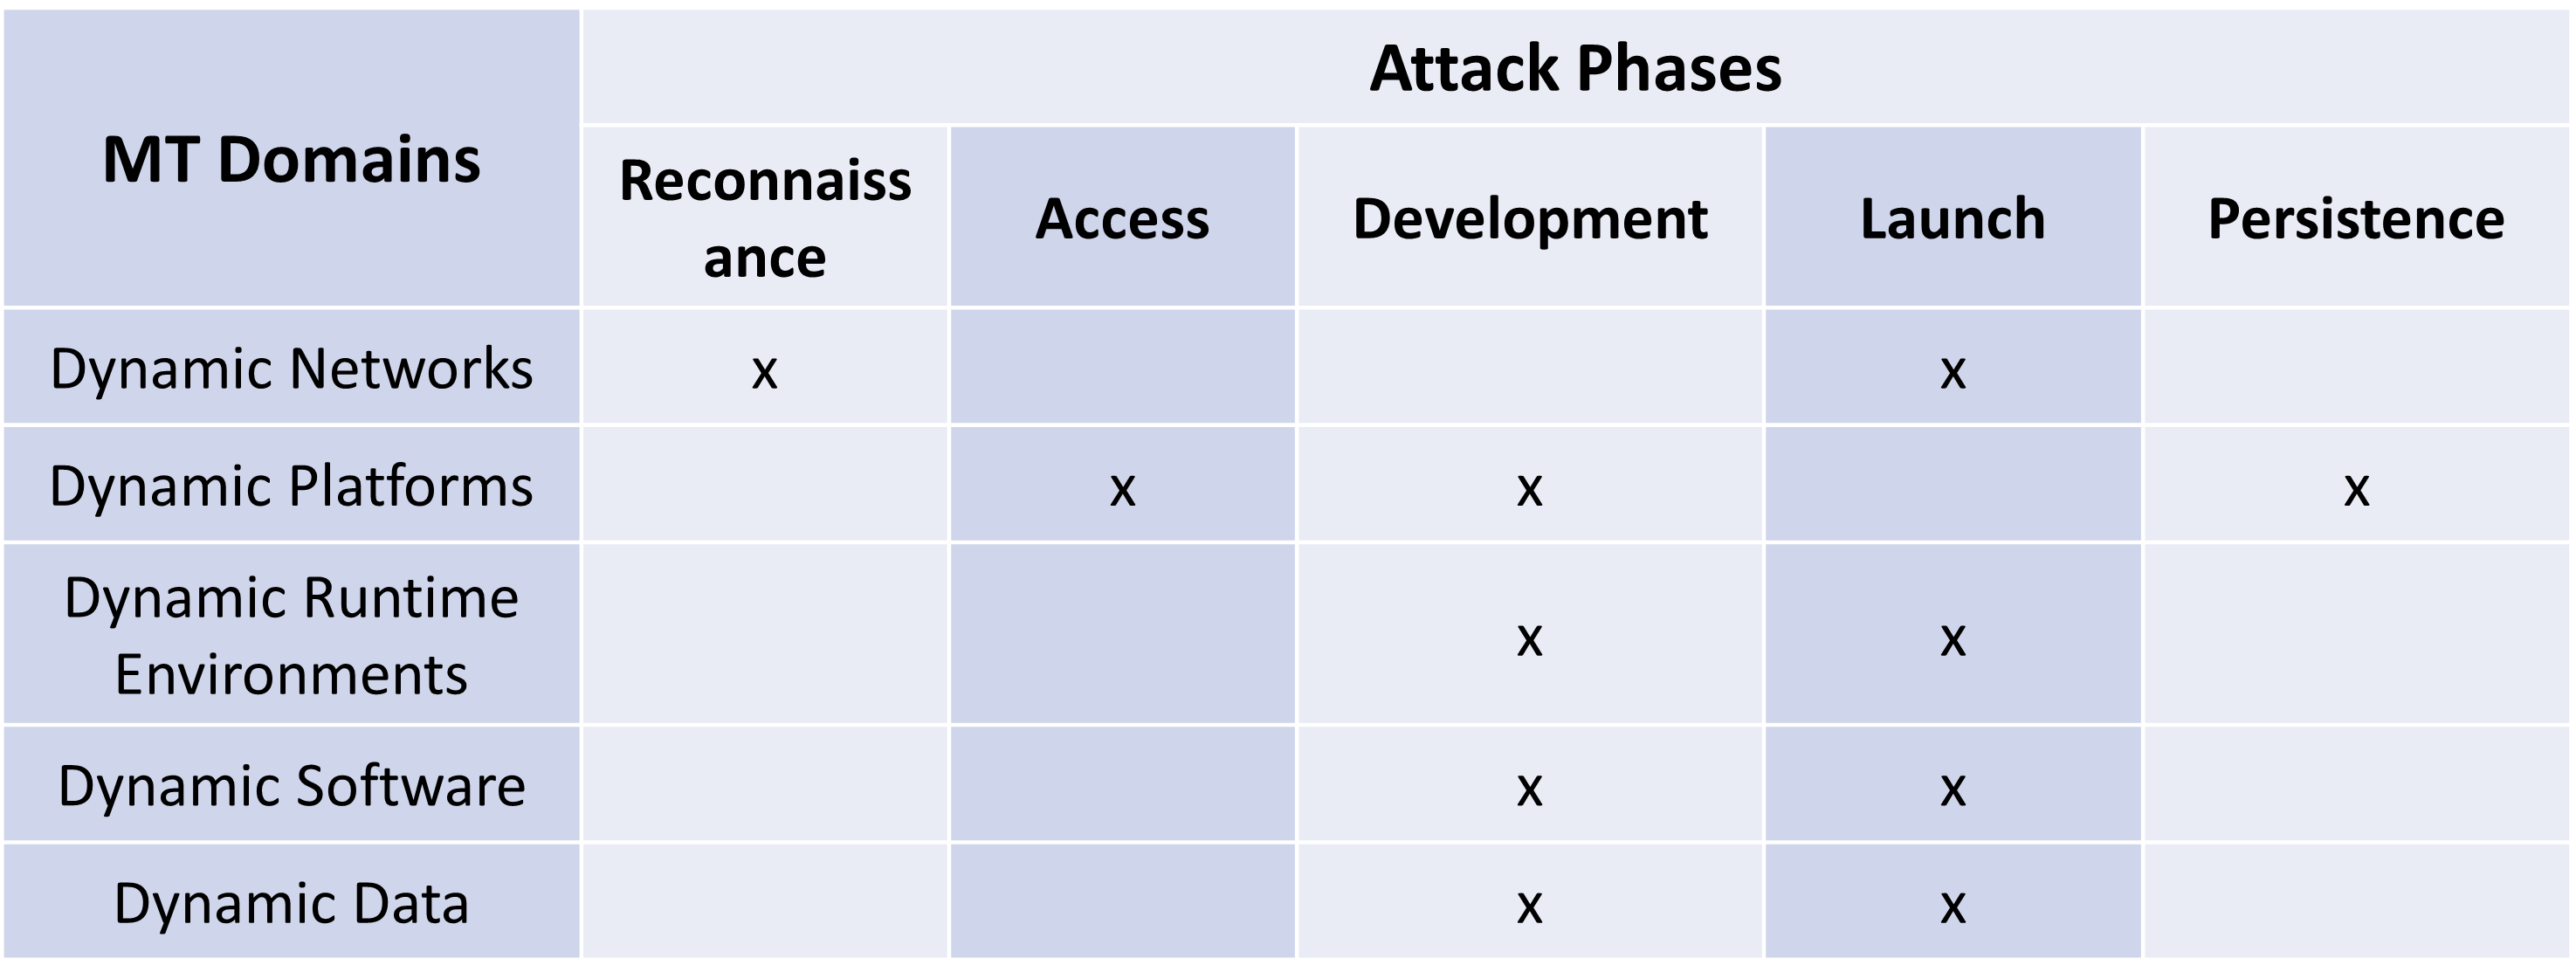
\includegraphics[scale=0.7]{assets/movingTargetDefenseAttack.png}
\centering
\caption{A Summary of the Moving Target Defense Domains and the Corresponding Attack Phase They try to Hinder~\cite{article:okhraviFindingFocus}.}
\label{table:movingTargetDefense}
\end{table}




\section{Internet of Things}
\cite{report:cern} gave a brief introduction about what the Internet of Things (IoT) is. It is about the collection and exchange of data through networked items embedded with electronics, sensors, software, actuators and a network connection. Examples of these items are physical devices, vehicles or buildings. These items can be controlled or sensed across an existing network infrastructure. This enables better integration of the physical world into computer-based systems, which has several benefits, such as reduced need for human intervention and economic benefits. But there are also major challenges for IoT, two of which are security and privacy. For example, a smart meter in a house knows when someone is at home, and this data is also shared with other devices and databases by companies that therefore also have this information.


\subsection{Current and Future Distribution of IoT Devices}
According to~\cite{website:statistaIoT}, there existed 11.3 billion IoT devices worldwide in 2021. By 2030, this number is expected to nearly triple to an estimated 29.3 billion devices.~\cite{website:fortuneIoT} estimated the global market size for IoT from 2022 to 2029. They estimated the market size to be 2,465.26 billion in 2029, which is significantly higher than the current 478.36 billion. Also interesting is the analysis of the current market share by end-use industry. At 21.5\%, the largest share of the end-use industry is accounted for by the healthcare market, followed by the manufacturing market and the IT \& telecom market. These three account for around 50\% of the total market share. Other examples include retail, transportation and banking, financial services and insurance.


\cite{website:gfuSurvery} has published a survey conducted in July 2021 on Smart Home solutions (consisting of IoT devices) and how many users are currently using them and how many users intend to use them in the future. 5 different groups were formed, which are shown in Table \ref{table:IoT}. It can be seen that some groups currently have a higher share and others a lower share, but the intended future use is significantly higher for each group. Another interesting insight is the breadth of the groups, ranging from lamps to security to garden and balcony. Thus, IoT devices can already be found in various places, and they will become even more important than they are today.  

\begin{table}[tph]
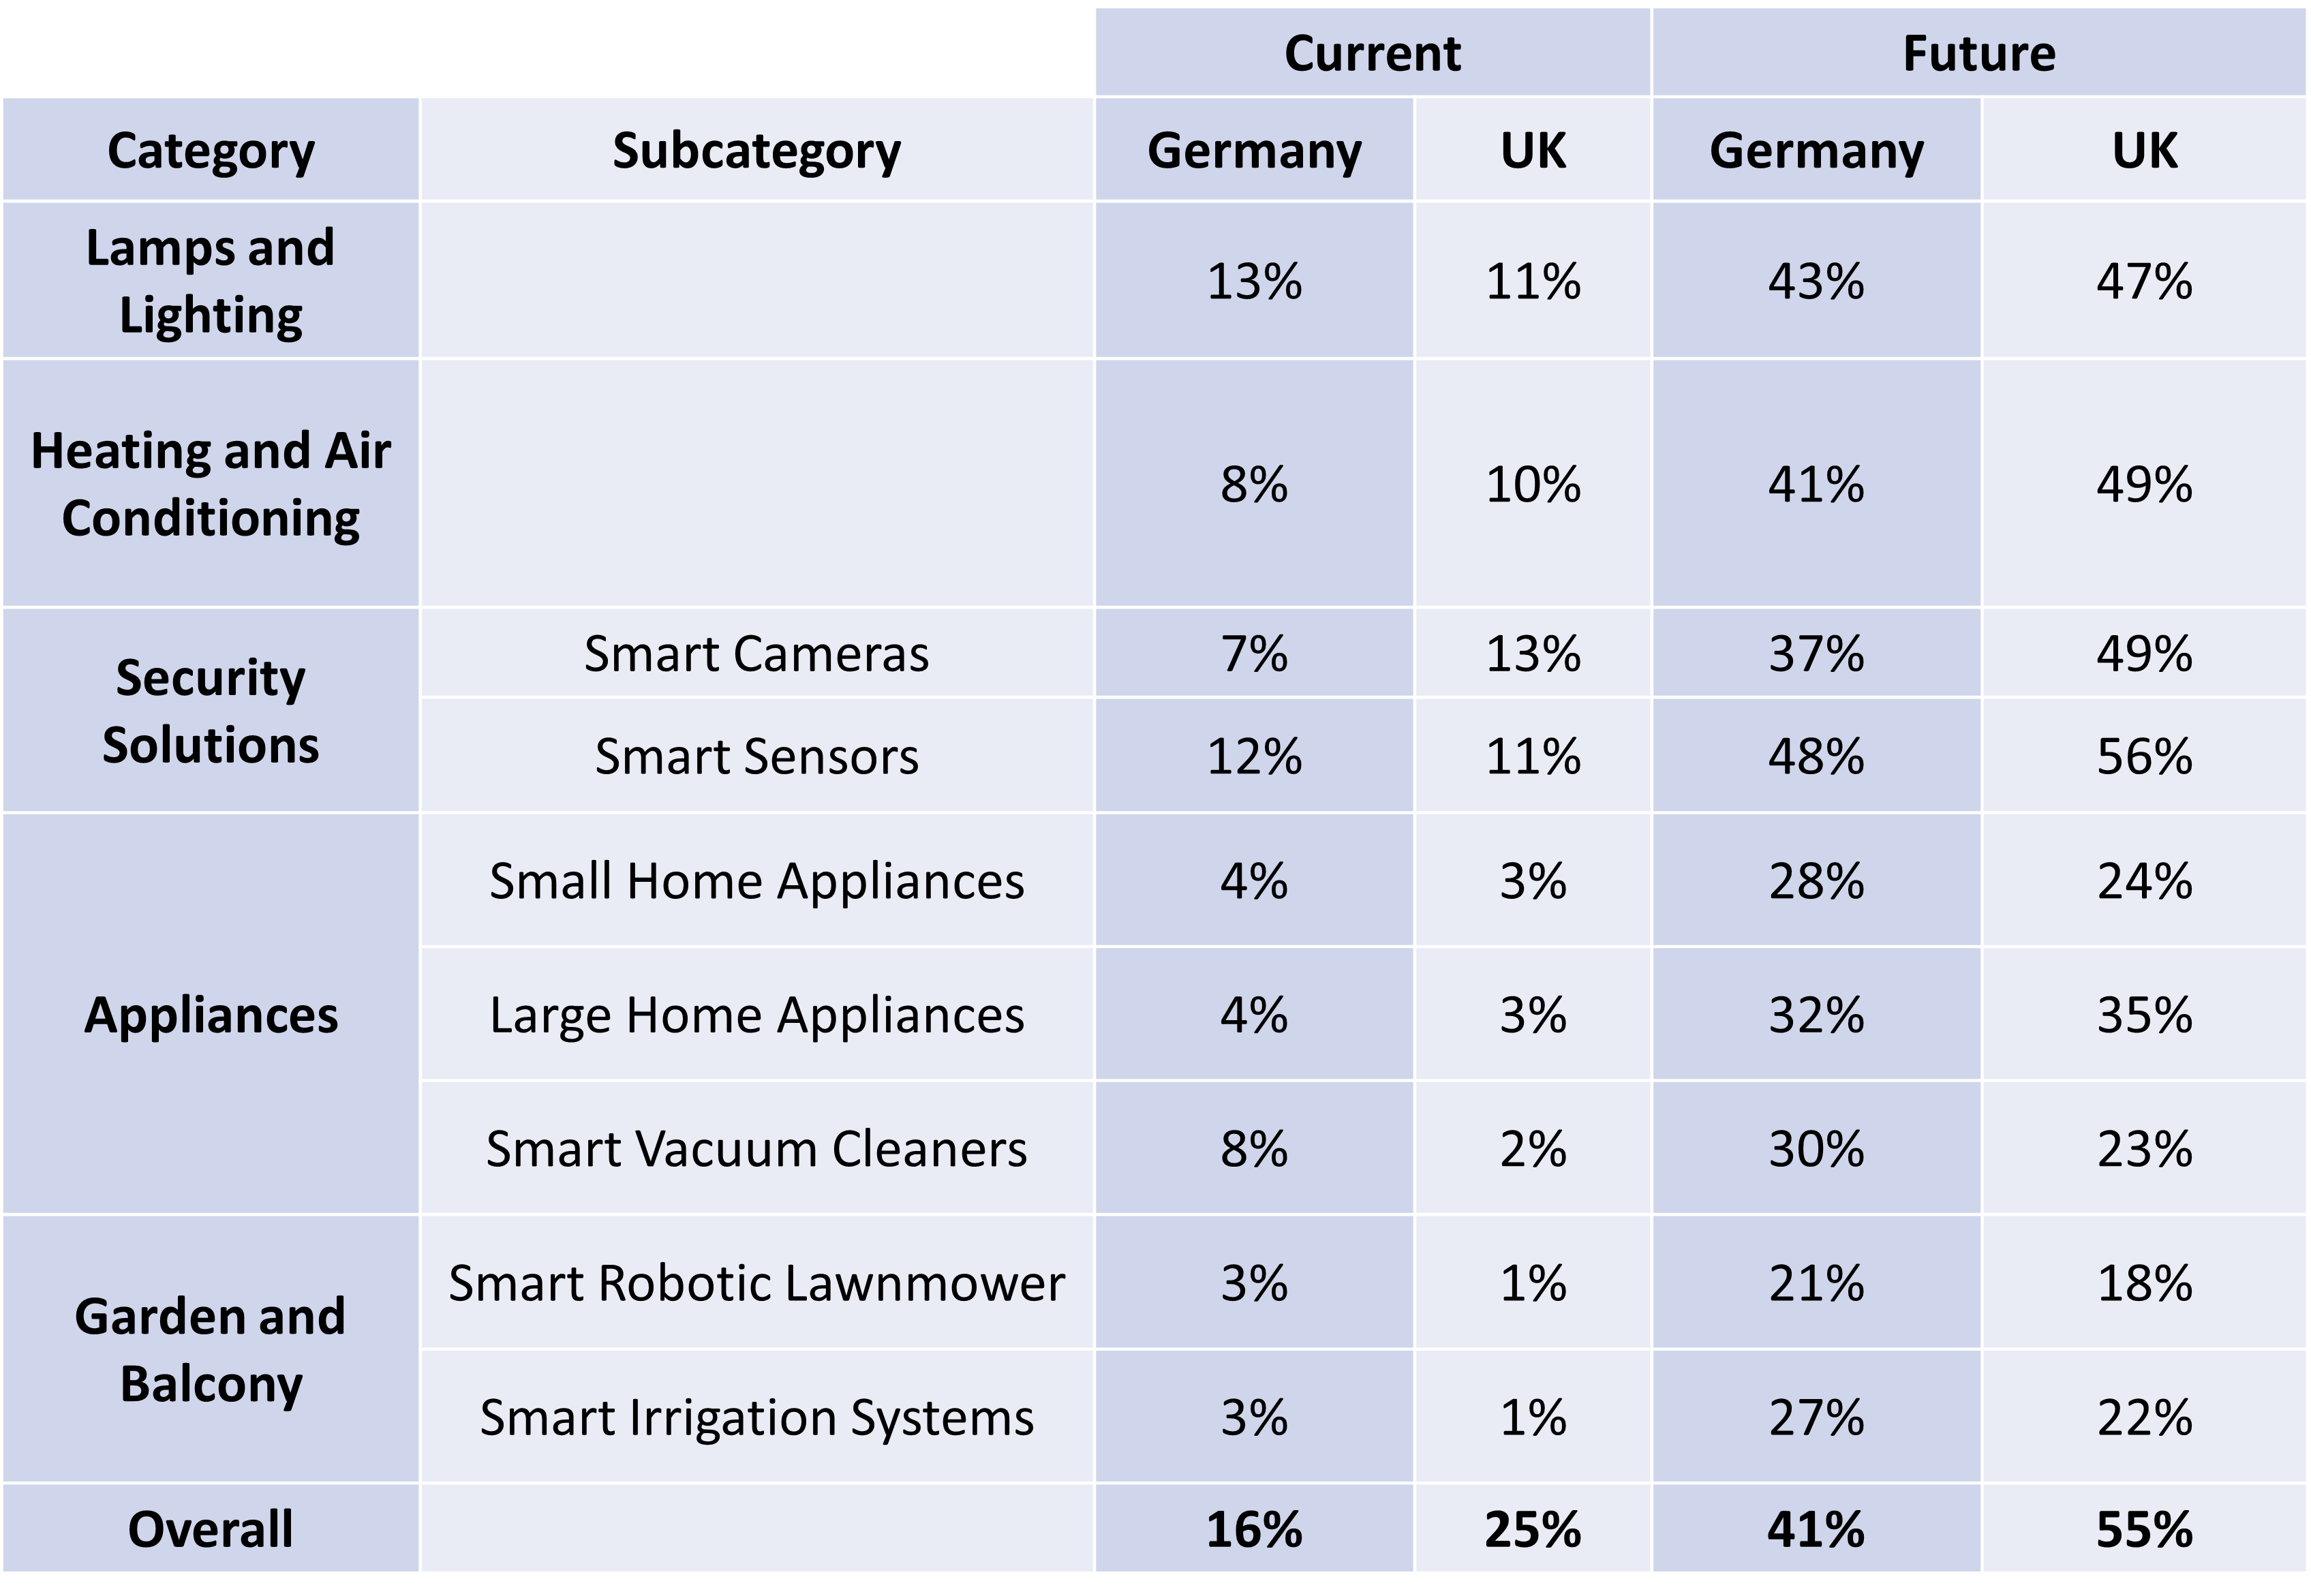
\includegraphics[scale=0.5]{assets/IoTTable.png}
\centering
\caption{Results of a Survey Regarding IoT Devices in Households Based on Data in Germany and the UK.}
    \label{table:IoT}
\end{table}



\subsection{Architecture}
\cite{article:Lombardi2021} published an article on a general overview between architectures, protocols and applications of IoT. The authors presented three different architectures that are most commonly found in the literature. 

The first architecture is a generic high-level architecture consisting of three layers, namely perception, network and application. The perception layer is the physical layer that interacts with the environment through information gathering and processing. Objects with computing power and the ability to interact with the outside world are an integral part of this layer. The network layer is the communication layer responsible for transferring data from the perception layer to the application layer. This layer includes all protocols and technologies required for this connection. An example of a protocol is 6LoWPAN, which stands for IPv6 over Low power Wireless Personal Area Network. The personal area network connects devices in a user's immediate environment, such as Bluetooth headphones with a mobile phone \cite{website:cloudFlarePAN}. The final layer is the application layer, which contains the essential software for a specific service. The data from the preceding layers is stored, processed, aggregated and filtered in this layer. The processed data is then made available to the IoT application.  

The second architecture is the service-oriented architecture. This architecture extends the three-tier architecture by adding a service layer between the application layer and the network layer. This service layer provides services to support the application layer and consists of several sub-services. The goal of this service-oriented architecture is to enable software and hardware reuse and to coordinate services. The architecture helps to connect different functional units through protocols and interfaces.   
% that are service discovery, service composition, service management, and service interfaces.


The third common architecture is the middleware architecture, also known as the five-layer architecture. This architecture is made up of five layers: the perception layer, the network layer, the middleware layer, the application layer and the business layer. The middleware layer, which aggregates and filters data received from the hardware, is an important layer. Various technologies are hidden in the middleware and standard interfaces are provided. This means that developers do not have to worry about compatibility between the infrastructures and the application and can therefore focus on the application development. 

The three architectures discussed can be seen in Figure \ref{graphic:IoTArchitecture}. Some additional architectures that also exist are the cloud-based architectures or the edge computing-based architectures.  



\begin{figure}[tph]
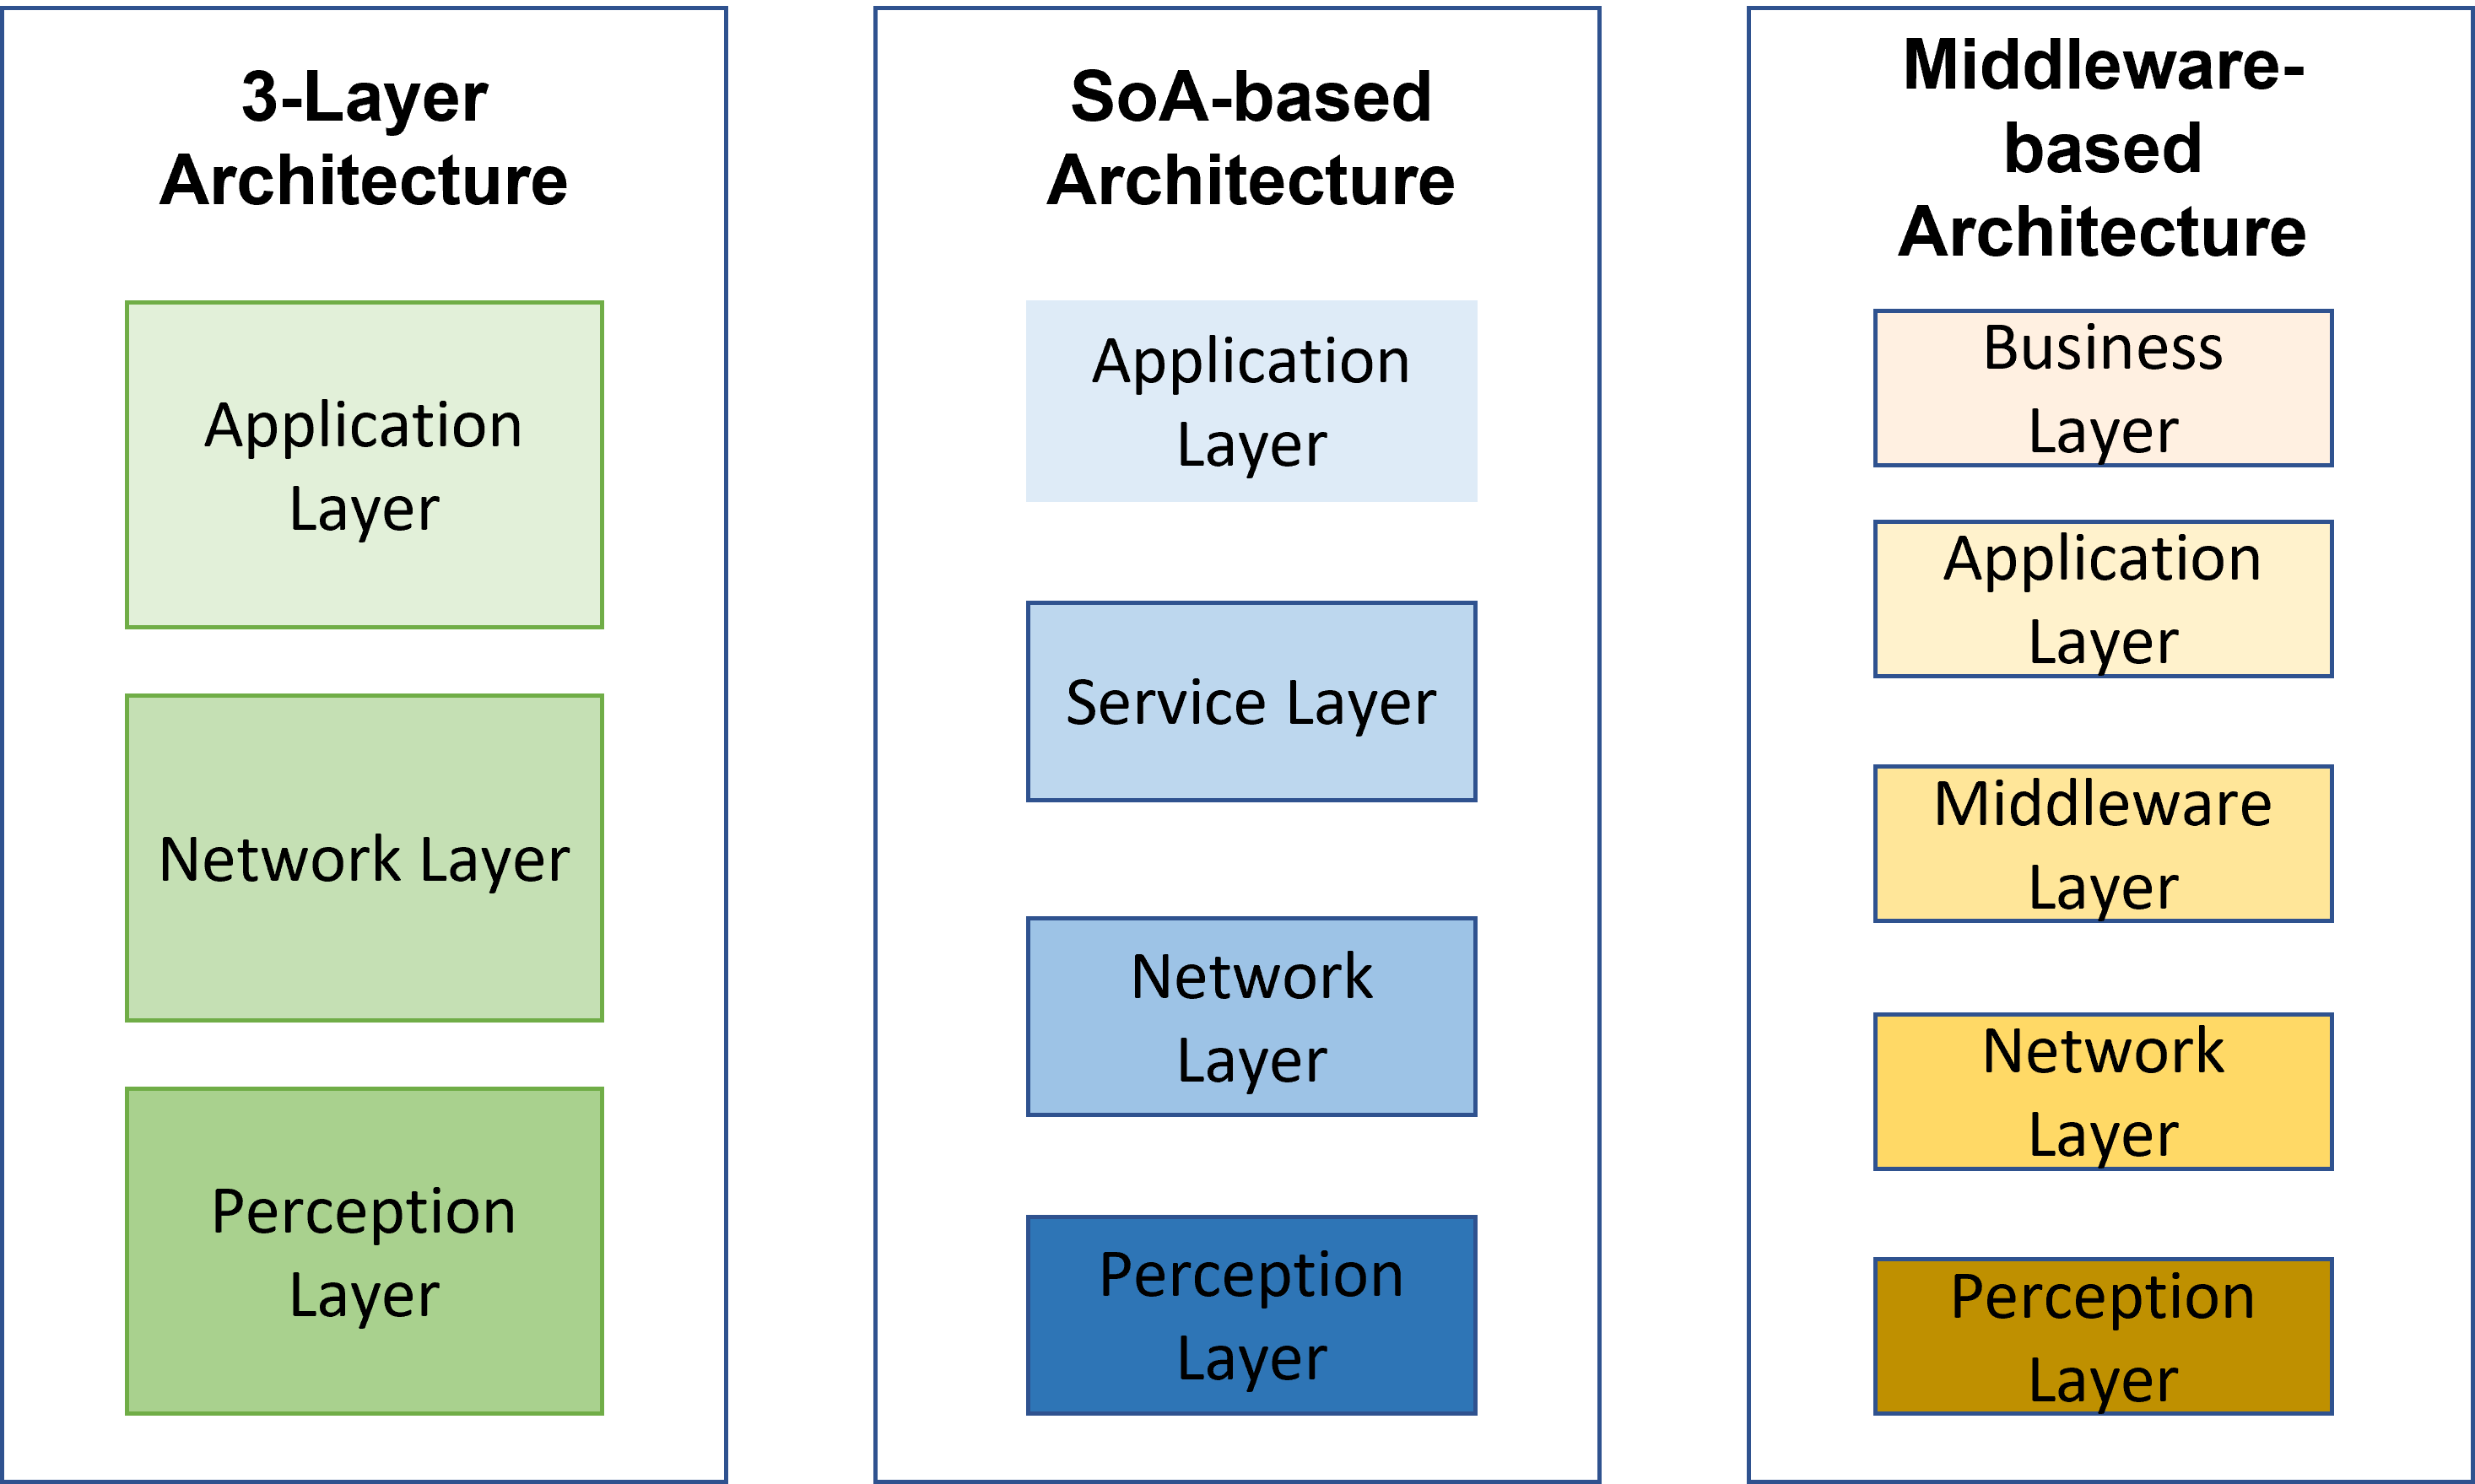
\includegraphics[scale=0.5]{assets/IoTArchitectures.png}
\centering
\caption{The Three Most Common IoT Architectures \cite{article:Lombardi2021}.}
\label{graphic:IoTArchitecture}
\end{figure}


\subsection{Hardware and Software Details of IoT} \label{sec:hardSoftware}
\cite{website:eclipseIoT} published a report on an IoT \& Edge Developer Survey with interesting insights. This survey was conducted in 2022 and 910 developers, committers, architects and decision makers were interviewed. One of the key findings for this thesis was that security concerns have almost doubled this year and are now in the top three challenges for developers, along with data collection \& analysis and connectivity. The most commonly used programming languages for constrained devices are Java, C and C++. In terms of the operating system (OS) for constrained devices, Linux distributions are the top choice with 43\%. FreeRTOS is in second place with 22\%. FreeRTOS is a real-time operating system for microcontrollers that is freely distributed under the MIT Open Source Licence~\cite{website:freeRTOS}. In third place is No OS/bare metal for constrained devices. The Linux operating system is further broken down into its distributions. Ubuntu makes up 23\% of all Linux operating systems, the second distribution is Raspbian with 20\%, the third is Alpine with 18\% and the fourth is Debian with 17\%. Interestingly, there are many more distributions in use, but they have a maximum share of 13\%. This information can be seen graphically in \ref{graphic:IoTOSs}.


In terms of architecture for constrained devices, ARM dominates. The most common architecture is ARM Cortex-M0/m0+ with 26\%. ARM Cortex-M3/ARM Cortex-M4 follows with 24\%. In third place is the ARM Cortex-M7 with 20\%.  




\begin{figure}[tph]
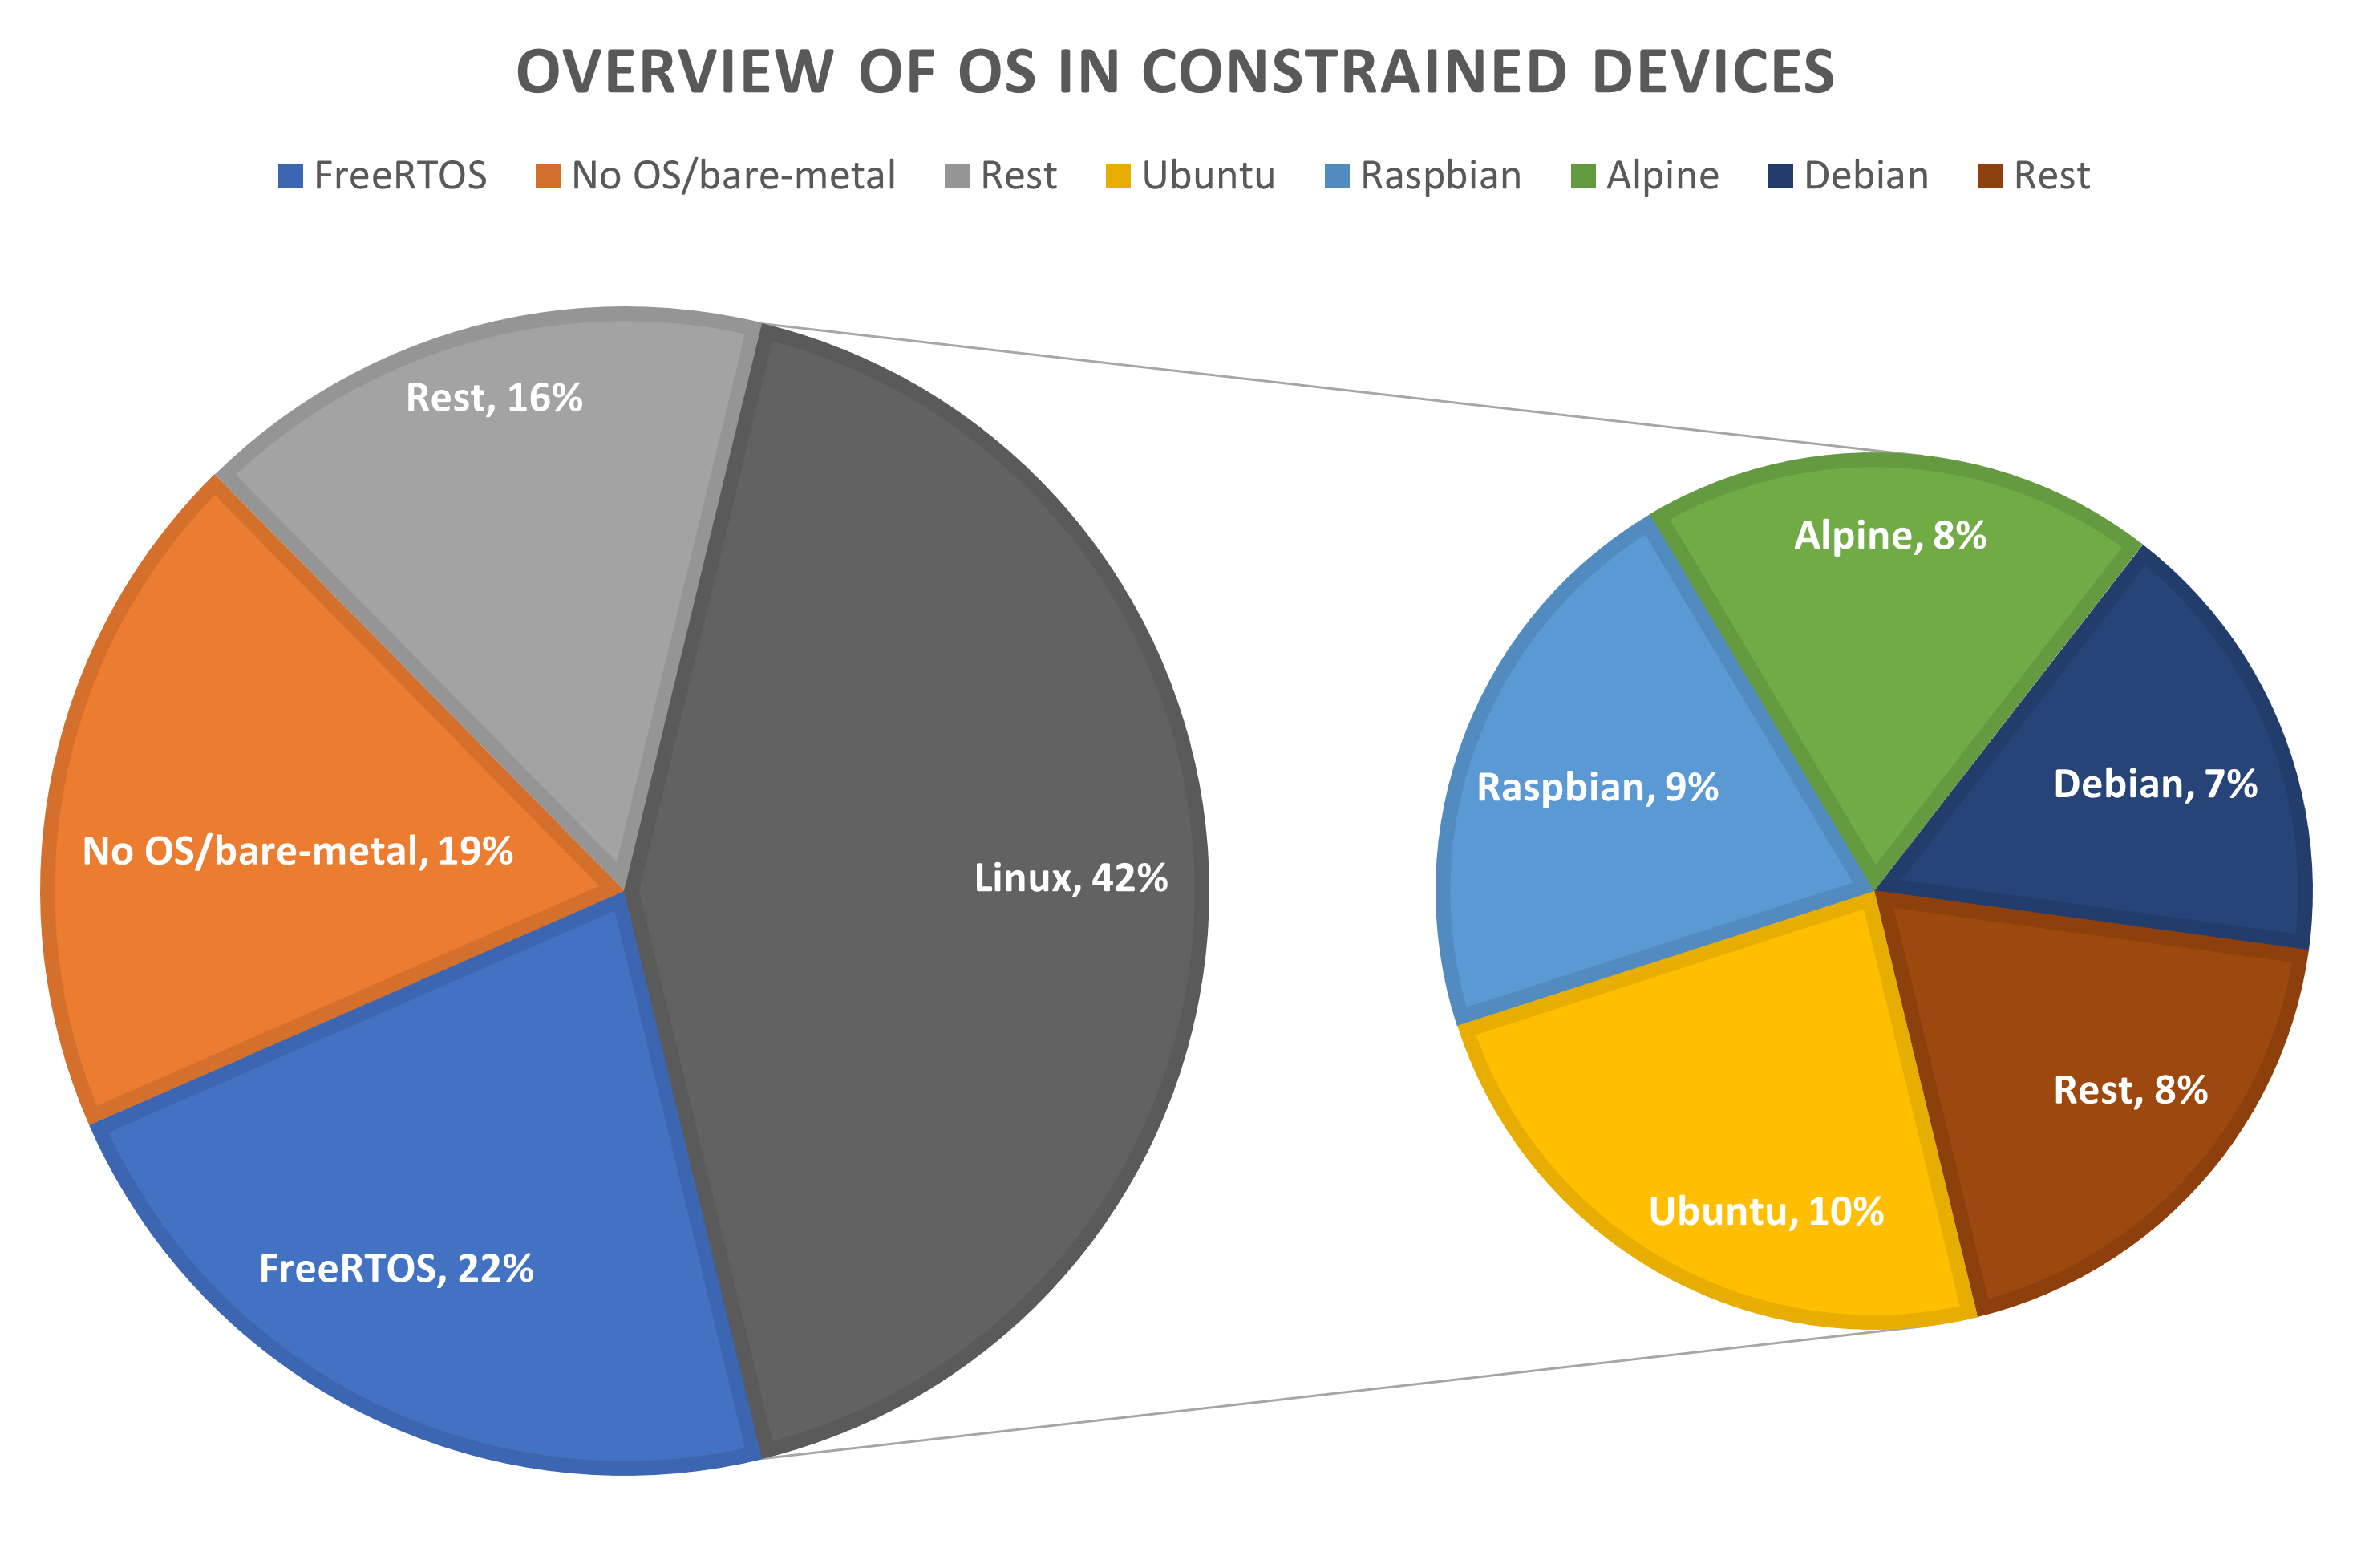
\includegraphics[scale=0.55]{assets/IoTOS.png}
\centering
\caption{The Most Commonly Used OSs in Constrained Devices.}
    \label{graphic:IoTOSs}
\end{figure}





\section{Malware and IoT} \label{section:MalwareAndIoT}
This section gives a general overview of malware, especially in the context of IoT devices. A more detailed analysis can be found in Section \ref{main:bashlite}, where Bashlite is analysed.

Malware or malicious software is a term used to describe malicious code or a program that is harmful to a system~\cite{website:malwarebytes}. Examples of malware or malware families related to IoT are Mirai, Bashlite, Tsunami or Hajime~\cite{article:surveyIoTmalware}. Mirai and Bashlite are probably two of the best known examples. Mirai, for example, was still highly prevalent in the first quarter of 2019~\cite{website:KasperskyAMalwareStory}. Bashlite, also known as Gafgyt~\cite{website:TrendMicroBashlite}, was already much less common in 2019~\cite{website:KasperskyAMalwareStory}, but other malware such as Mirai has inherited 
 from its source code~\cite{article:surveyIoTmalware}.

 
\cite{article:evOfBashlite} gave a brief overview of Bashlite and Mirai and how they are used to create botnets. The rest of this paragraph is based on that article.
Since the source code of Mirai is based on that of Bashlite, they share some similarities. For example, both infect IoT devices that can be accessed with known and/or vulnerable authentication credentials. They also both aim to create botnets. These botnets have different components. The command and control (C\&C) servers send commands to the infected devices and essentially act as the operator's interface to the botnet. The bots are the infected devices that make up the botnet. They execute the commands received from the C\&C servers. There are also scanners that identify vulnerable devices by looking for Telnet and SSH servers that the scanners attempt to log into. Loaders download and run the malware of the botnet after logging into the vulnerable devices. Malware servers provide resources such as executable binaries to the botnet. A possibly distributed database stores collected information such as scan results or active bots.

Such botnets can be used for different purposes~\cite{website:IBMIoT}, which  are described below. The first purpose is the aforementioned DDoS attack. The idea is to attack a target by sending so much traffic from many different machines that the target cannot handle the volume, eventually taking the target down. Another use for botnets are spam bots. Using botnets, spam can be sent from IP addresses that are not yet known to be spam relays and therefore not yet blocked by system administrators. A third purpose are crypto mining bots, which can be used to mine cryptocurrencies such as Monero. These malware require a device with sufficient processing power (e.g. smartphones), so constrained devices are not optimal for such malware to infect.

According to~\cite{article:DDoSinIoT}, there are five main reasons why IoT devices are advantageous for creating botnets:
\begin{itemize}
\item IoT devices often operate around-the-clock, they do not have on-off cycles like laptop and desktop computers. 
    \item IoT devices are poorly maintained. A very common problem is that devices are set up and then forgotten about as long as they are working properly. 
    \item IoT devices are capable of generating significant distributed denial of service (DDoS) attack traffic, similar to the attack traffic generated by modern desktop systems. 
    \item IoT devices are often either non-interactive or require minimal user intervention, resulting in infections going unnoticed. 
\item IoT vendors favour usability and user-friendliness over security, resulting in weak protection.
\end{itemize}

The last item in the enumeration includes a number of known vulnerabilities~\cite{website:IBMIoT}. The first are weak passwords to make it easier to set up and use the device. These passwords are many times printed in the user manual or even outside the packaging. As the credentials are often the same for all the same devices, this is a huge problem. Even if the credentials were not so accessible, they are often predictable combinations such as "admin/admin". In addition, many devices lack encryption. Such security features are often not even considered. In addition, vendors sometimes add hidden access mechanisms, called backdoors, to devices. They might do this to make it easier to support the device, but it could also be used by hackers. An example is an open port on the device that cannot be closed. 


\subsection{IoT Malware Statistics}
\cite{website:KasperskyAMalwareStory} published a report in which the authors researched attacks on IoT devices using honeypots. The authors mentioned that such honeypots are the best option to track attacks, catch malware or just get a general overview. This subsection is based on that source. There exist three different common types of honeypots. 

\begin{itemize}
    \item Low-interaction honeypots simulate services such as SSH, Telnet and web servers. The attacker is fooled into thinking that this is a real susceptible system and attacks the honeypot.
    \item High-interaction honeypots are real systems that have the advantage of running fully POSIX capable systems. POSIX is a standard defined by the IEEE~\cite{website:IEEEPosix}. This standard helps to maintain compatibility between operating systems~\cite{website:linuxHint}. As these honeypots are real systems, it is important to take action against the malicious activity of the malware (e.g. prevent further systems from being compromised). 
    \item Medium-interaction honeypots are a combination of low-interaction and high-interaction honeypots.  
\end{itemize}

The authors collected data from more than 50 honeypots around the world over the course of more than a year.

In the first six months of 2019, the Telnet honeypot detected more than 105 million attacks from 276,000 attacking IP addresses. This is significantly more than the 12 million attacks from 69,000 IP addresses in the first half of the previous year. The most attacking IP addresses came from Brazil and China with 30\% and 19\% respectively. Egypt, Russia and the US followed with 12\%, 11\% and 8\% respectively. Regarding the top malware threats that attacked the Telnet honeypot, 6 out of 10 were Mirai variants. There are several reasons for this, including the public availability of the malware and its ability to create bots of any complexity and for any hardware configuration. The NyaDrop family of malware was the most common, accounting for around 39\% of all attacks. This is a Linux trojan that targets IoT devices and specifically the MIPS CPU architectures~\cite{website:comodoAntivirus}. In second, third, fourth and fifth place were the Mirai variants with 22\%, 12\%, 2\% and 2\% respectively. 

Another interesting finding was the most common combination of credentials tried. "support/support" was tried 2,627,805 times, "root/vizxv" was tried 2,376,654 times, and "admin/admin" was tried 2,359,985 times in the first quarter of 2019. The second is the default combination for connecting to a vulnerable camera from Dahua via Telnet~\cite{website:dahuaDefault}. The last interesting finding the authors made was in terms of the ports targeted by the malware. TCP ports were clearly the most targeted, with only a small number of attacks targeting ICMP and UDP ports. Unfortunately, the authors did not provide statistics for other protocols such as SSH in the same depth as they did for the Telnet protocol.  


\subsection{P2P IoT Botnets} \label{subsection:P2PIoTBotnets}
The botnets described so far correspond to the typical IoT botnet~\cite{website:trendmicroTheFuture}. Adversaries control the botnet from a C\&C server that controls various infected devices. This means that taking out the C\&C servers renders the entire botnet useless, regardless of how many bots are connected to the system~\cite{website:trendmicroTheFuture}. While taking down many C\&C servers can be cumbersome, it can also be a convenient solution against botnets. For example, this strategy was used against the Andromeda botnet~\cite{website:europol}. Several international authorities took action against domains and servers that were spreading the Andromeda malware. This involved, for example, sinkholing  1500 domains. Sinkholing is when traffic is redirected to a server other than the intended one, such as one controlled by law enforcement authorities~\cite{website:europol}. 
However, this solution vanishes as soon as the botnet is set up as a peer-to-peer (P2P) network.~\cite{website:trendMicroUncleanable} wrote a technical briefing on the development of IoT botnets in combination with P2P networking. The rest of this subsection is based on that source.

Unlike a botnet with a central server, a P2P network is much more robust. The authors use BitTorrent as an example because it has withstood the test of time, having been used to share illegal content for over 20 years without the authorities being able to shut it down. In the case of a P2P IoT botnet, each bot would need to be disinfected separately, as there is no central server. This is also a problem caused by the insecurities of IoT systems, as discussed in Section \ref{section:MalwareAndIoT}. In the case of a desktop environment, mass cleanup would theoretically still be possible, e.g. by antivirus vendors, but this is not an option for IoT devices because there is no antivirus protection. Fortunately, there are not many P2P botnet families yet, the authors stated that they have only seen five families so far, and they also suspect that they are not common at the moment. Although they do not know the actual number of infections, they find it worrying that the rate at which P2P botnet malware appears is increasing. The authors conclude that this indicates an increased interest in creating P2P botnet malware. The authors then briefly describe each of the five malware families. One of these five is described below to give a general idea.

The most recent malware mentioned by the authors is "HEH". HEH is written in Go and scans and infects via Telnet port 23 and port 2323 with hardcoded credentials and brute-forced passwords. The malware starts by randomly selecting an IP address and then uses an algorithm to derive the P2P port from that IP address. Thus, no list of IP addresses and ports is required. Once a victim is infected, it attempts to connect to other peers. Additionally, the malware stops the HTTP service and starts its own service instead, which acts as a download site for infected devices. The P2P protocol has 5 operation codes, 4 of which are for synchronisation and one for receiving commands. The latter accepts various instructions such as 'exit', 'attack', 'execute' and 'self-destruct'. According to the authors, the last command was particularly interesting because it is unusual for a bot to be able to destroy itself.


The authors also shared their thoughts on the future development of P2P IoT botnets. They emphasized the importance of making money as an incentive for cybercriminals to develop malware. Since these incentives are critical to development, it makes sense to take a look at how these incentives have evolved.
Routers are an interesting target for attackers because they act as an entry point into a home network. An infected router also offers many opportunities such as man-in-the-middle attacks or information theft. Additionally, an infected router allows lateral movement to infect other unsecured devices on the network. The authors also mentioned that, in terms of financial incentives, a distinction needs to be made between the pre-Covid 19 era and now, due to the increase in home offices. For example, an infected home router could now be an entry point into a company, which could be a possible financial incentive for adversaries. There is also a general risk that a successful attack will motivate other cybercriminals to do the same. For example, the authors predict that once a P2P IoT botnet is successful enough, all other botnets will start using P2P capabilities as well.
As a result, there is a realistic risk that such P2P malware will be further developed and distributed, but this is highly dependent on the financial incentives.

As this chapter has shown, there are many problems with the security of IoT devices. There are several reasons why IoT devices are susceptible to malware, such as poor maintenance or a focus on usability rather than security~\cite{article:DDoSinIoT}. Infected IoT devices can be used for malicious behaviour. One problem are botnets, where infected devices act as bots that execute commands sent by an adversary. As~\cite{website:KasperskyAMalwareStory} noted, there were about 9.5 times more attacks in the first half of 2019 (105 million) than in the first half of 2018 (12 million), which is an extreme increase. Another growing problem are P2P IoT botnets. Even if they are not very prevalent currently, it is certain that these P2P botnets can become a major threat in the future because they are almost unkillable. Each of the above points makes it clear that a way to defend against such threats is essential.



\section{Cooperative Defense}
There were not many resources available on the subject of cooperative defence. The ones found are presented in this section.

\cite{article:Zhang} is a relatively old paper from 2005 in which the authors aim to detect DDoS attacks in the intermediate network. The goal was to enable a DDoS attack detection system to share information, rather than to improve a currently available detection method. To achieve this, they proposed a dynamic defence infrastructure consisting of independent defence nodes and assumed that a DDoS attack heading towards a victim would consume more bandwidth than a normal use of the Internet. For scalable and resilient communication to exchange attack information, the authors designed a directional gossip mechanism. Each defense node sets a limit on the amount of traffic it deems malicious, based on its own defense strategy. This usually results in a high number of false positives due to the dynamic nature of the Internet. The defense accuracy is improved by the gossip mechanism, which helps to transmit information between nodes. During this information exchange, the rate limit is adjusted at each individual defence node.
When the mechanism for aggregating information converges, the defense node's rate limit will have roughly global information of the attack, which allows it to more accurately block/drop malicious traffic.


\cite{article:RodiguesBlockchain} and~\cite{article:RodriguesEvaluation} proposed and evaluated a cooperative defence mechanism based on the blockchain. The authors presented a scenario in which a web server in an autonomous system is under a DDoS attack from devices hosted in other autonomous systems. An autonomous system is a network or group of networks which share a single routing policy~\cite{website:cloudFlare}. A routing policy contains a list of IP addresses controlled by the autonomous system and a list of other autonomous systems to which it is connected~\cite{website:cloudFlare}.
In this scenario, the web server relies on the defences of the autonomous system where the server is located. As it is better to block malicious traffic close to its origin, this approach is not ideal. This is where the blockchain comes in. The idea is to store the attacker's IP address in a smart contract created by the collaborative defence participants. In this way, subscribed autonomous systems on the Ethereum blockchain receive an updated list of addresses to be blocked and also confirm the authenticity of the attack. Once the other autonomous systems receive the updated list and confirm the attack, the mitigation strategies in the autonomous system can be triggered to block malicious traffic close to its origin.



\chapter{Related Work}
This chapter presents related work. The first section presents an article on the current state of research on MTD in IoT. The second section presents related work in the area of MTD frameworks for IoT devices. The last section gives an overview of specific IoT techniques and explains how they relate to the work at hand. 

\section{State of Research of MTD in IoT}
\cite{navas:2021MTDWhere} did a literature review analyzing existing MTD for IOT techniques. This section is based on that source. The authors defined four research questions, all of which are of interest in the context of this thesis. The first research question concerned the number of proposals for MTD techniques that exist for IoT. They concluded that since 2013, 32 novel proposals have been proposed for the IoT domain. In contrast, more than 80 different general purpose MTD techniques have been proposed from 2009 to 2018~\cite{website:surveyOfCyberMovingTargets}. 

The second research question was related to the characteristics that can be observed in MTD techniques for IoT. For this question, the authors created an MTD taxonomy showing the distribution of these 32 techniques grouped in the MTD domain mentioned in Section \ref{section:MTD}. The dominant techniques are the networking techniques with 54\%, followed by the dynamic runtime environment techniques with 20\%. Software and data techniques follow with 13\% and 10\%, respectively. Dynamic platform techniques have the smallest share with 3\%. Figure \ref{graphic:IoTShare} shows these shares graphically. These shares differ from those of the general-purpose MTD techniques, where, for example, the dynamic network techniques account for only about 21\% or the dynamic platform for about 20\%. A possible reason for this is that recently there has been an increasing interest in network-based MTD techniques~\cite{navas:2021MTDWhere}. 
 
 \begin{figure}[tph]
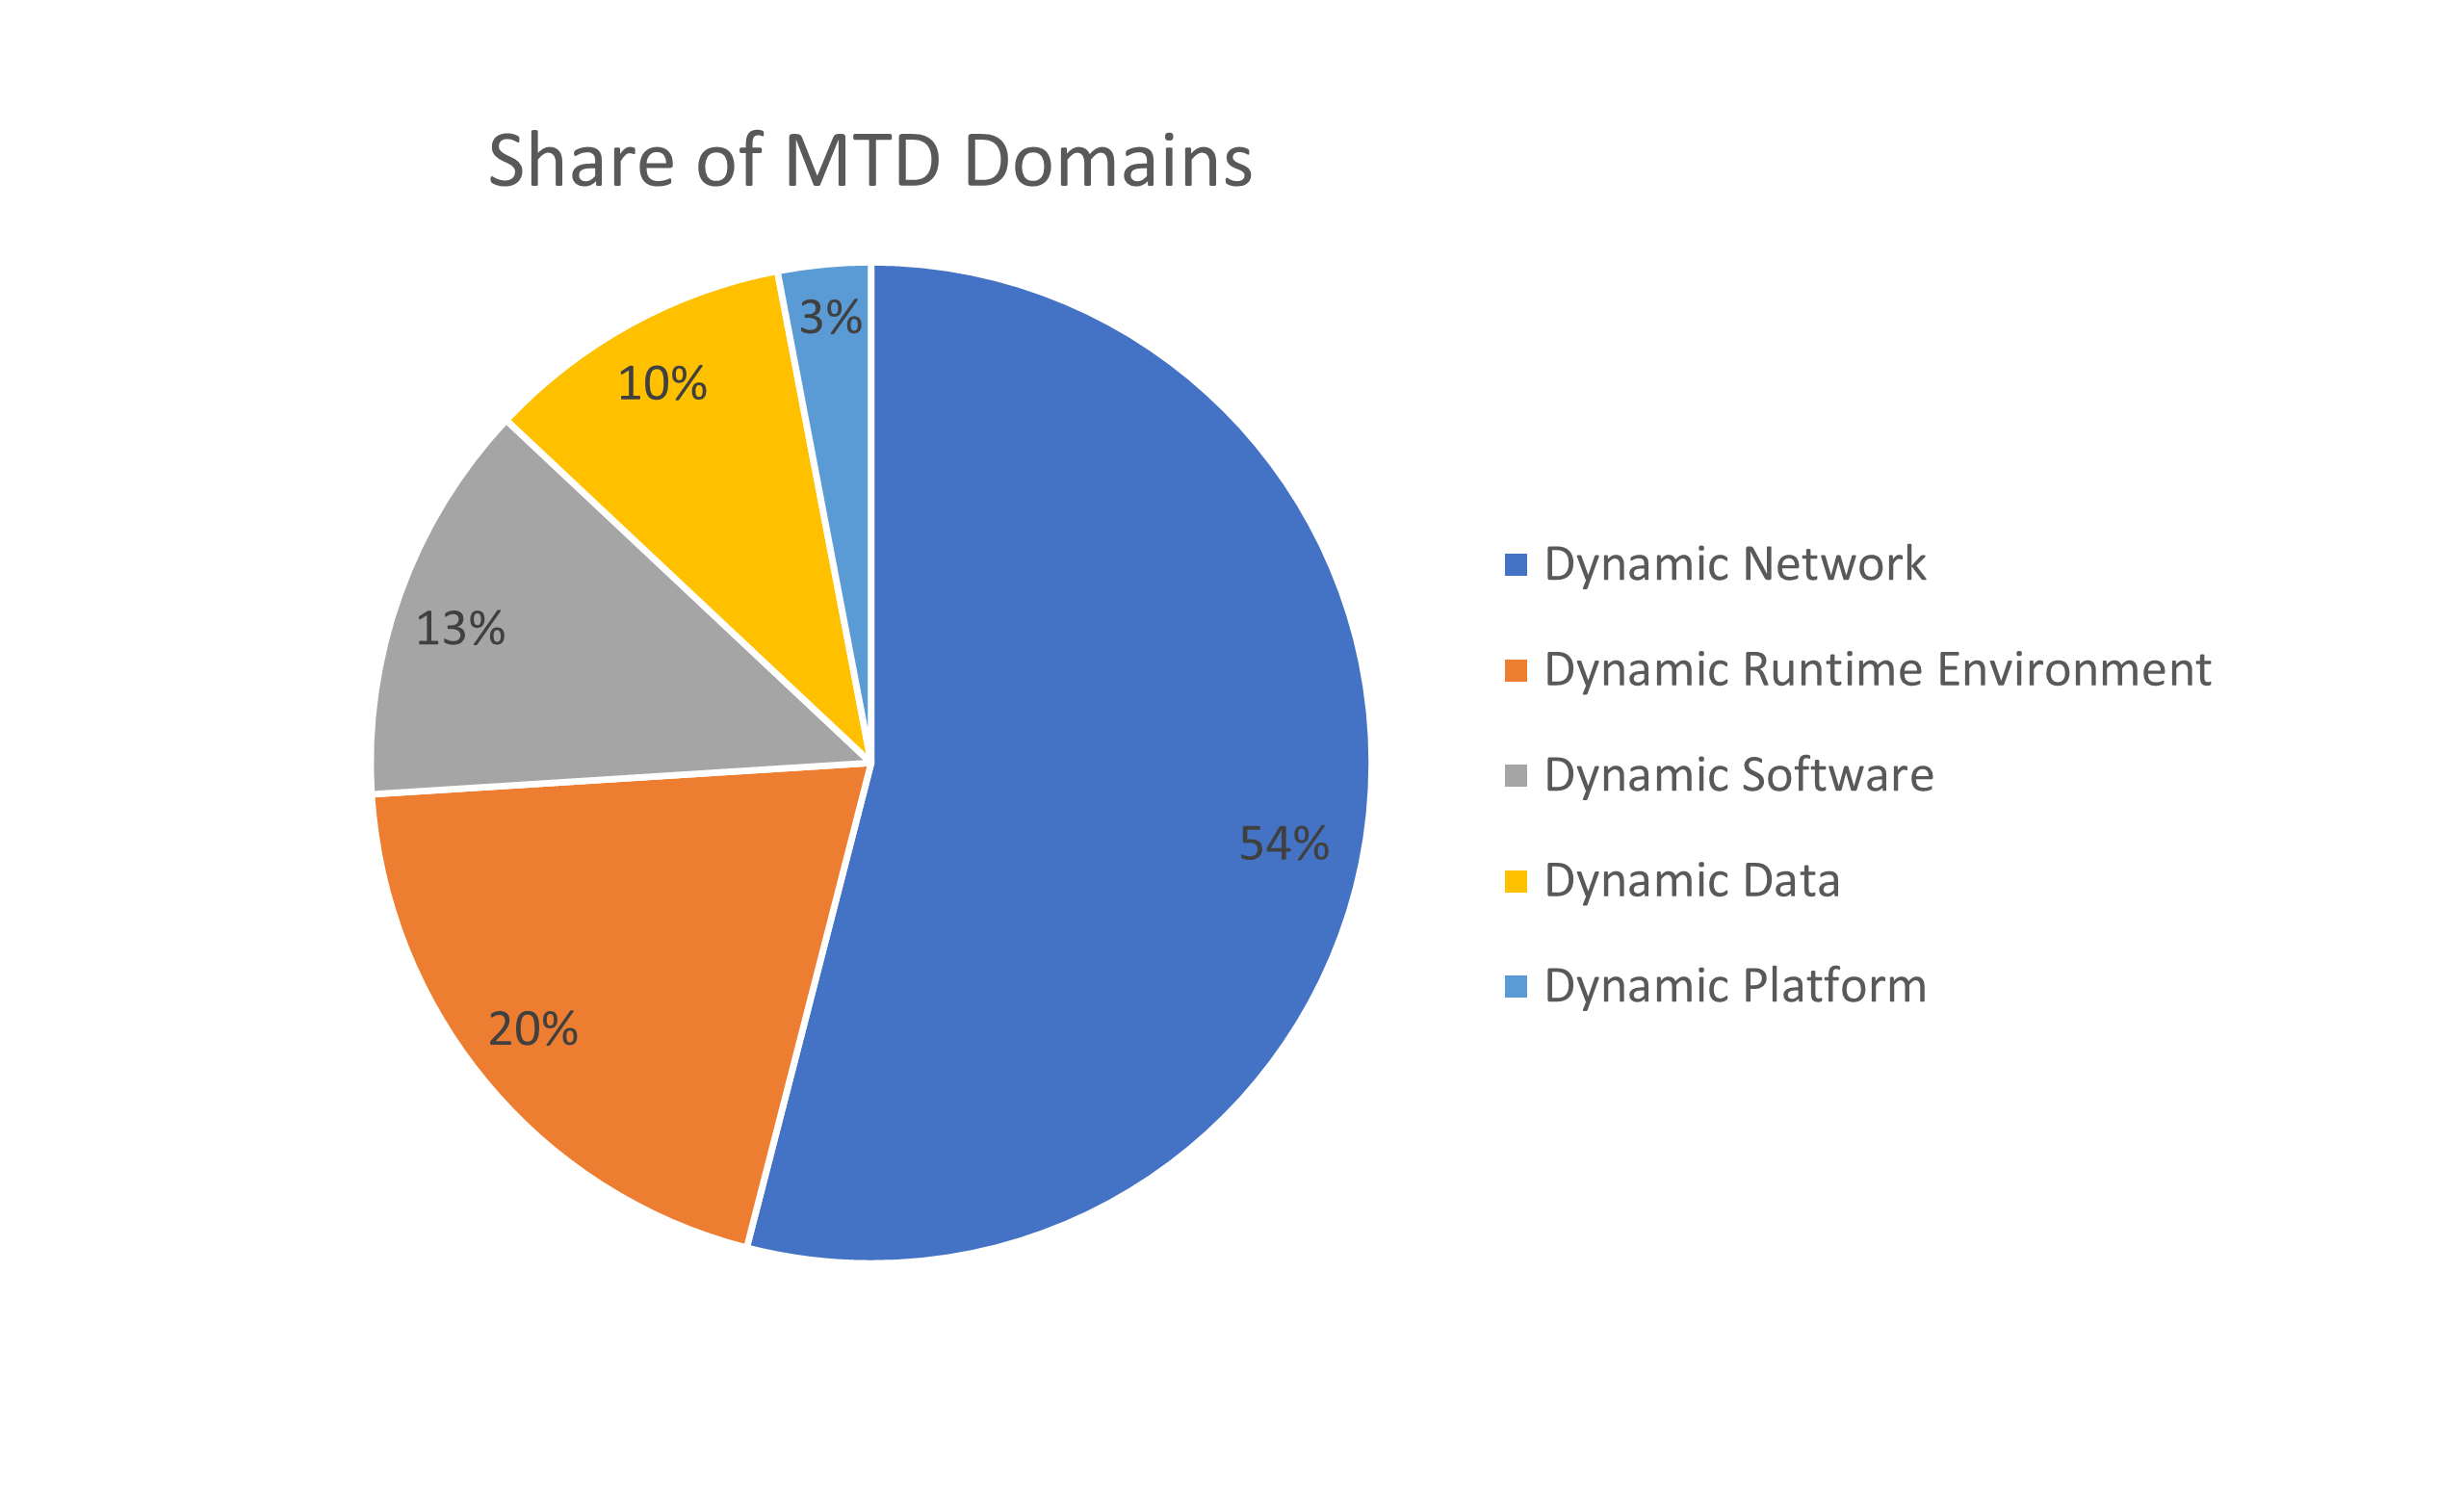
\includegraphics[scale=0.6]{assets/shareOfMTDDomains.png}
\centering
\caption{Share of IoT MTD Techniques Grouped by MTD Domains~\cite{navas:2021MTDWhere}.  }
    \label{graphic:IoTShare}
\end{figure}

The third research question was how sound the security foundations of the proposed techniques are. To answer this question, the authors classified each of the 32 techniques into three different cryptographic categories. The first category, which includes twelve techniques, completely lacks cryptography or uses a random process without providing further information about it. The second category either uses cryptographic techniques that are known to be vulnerable or uses custom cryptography without proof. Nine techniques fall into this second category. The last category is the one that has adequate security foundations, such as using state-of-the-art cryptography like SHA256. There are eleven techniques in this category. The authors point out that although they have simplified the measurement of security, 32\% is a small value considering that the central goal of MTD is to improve security. The fourth research question is the most interesting and relates to the extent to which the proposals are applicable in a real-world IoT deployment. To answer this, the implementation and evaluation aspects of the proposed techniques were examined by the authors. They concluded that 50\% of the proposed techniques show very strong or strong evidence that they can be used in a real IoT deployment. Another 25\% of the techniques show mild evidence, and another 25\% have weak to no evidence that they can be used in a real IoT deployment. The authors conclude that these are encouraging results.


\section{MTD IoT Frameworks}
\label{section:MTDFramework}
%Despite a thorough literature research, it was not possible to find any other articles on the topics of cooperative defense, IoT, and MTD. In particular, the cooperative defense part was missing, so the focus lies on articles that studied MTD and IoT in this chapter.   

\cite{article:vonderAssen} presented an MTD framework aimed at mitigating multi-purpose malware. The framework consists of two modules, the MTD decision module, which decides when to deploy an MTD mechanism, and the MTD enforcement module, which decides what MTD mechanism to deploy and how to do that. The authors distinguished between a rule-based proactive approach and a machine-learning based reactive approach to determine when the MTD mechanisms should be executed. They were able to detect normal and malicious behavior in about 10 seconds.~\cite{article:Cedeno} wrote a bachelor thesis, whose results are part of~\cite{article:vonderAssen}. This thesis is about mitigating cyberattacks on resource-constrained devices using MTD. To achieve this, the author developed an architecture consisting of three main components, an \textit{MTD Deployer Server}, an \textit{MTD Deployer Client}, and the MTD solution itself. The \textit{MTD Deployer Client} serves as an interface for external programs to notify the \textit{MTD Deployer Server} of an attack. After the \textit{MTD Deployer Server} receives an attack report, it searches for the appropriate MTD solution, whereupon the \textit{MTD Deployer Server} launches the appropriate script of the MTD solution to mitigate the attack on the affected machine. This architecture was also the basis for the thesis at hand.


\cite{article:mercado-velazquez} created a framework that helps to answer the fundamental design questions (What, How, When) described in Section \ref{section:MTD} by using five different variables: attack success probability, system downtime, CPU time, energy consumption, and memory usage. The framework starts with policies, i.e., desirable goals and targets to be achieved. Then some strategy parameters (what to move, when to move, and how to move) are defined. These parameters are then applied to the IoT system which will be continuously attacked. During these attacks, the five variables are measured. These variables are then analyzed using multiple criteria decision analysis. The result of this analysis is compared to the targets defined in the policies. Depending on this comparison, either the final strategy parameters are fixed or different strategy parameters need to be created and the framework starts over.
Finally, the authors used this framework to select the most suitable "when to move" parameter for a proposed MTD technique.


\cite{NavasDefenseFramework} proposed a generic MTD framework for IoT called IANVS. This framework consists of four different components that should facilitate the implementation of MTD in distributed systems, since in such systems the parties involved need to agree on the MP value. The four components are

\begin{itemize}
    \item An authenticated key establishment mechanism called AKE. This provides a secret cryptographic key that only trusted parties of the MTD strategy must know.  
    \item An authenticated state synchronization mechanism called Auth-SYNC. This provides a system state value that must be fresh and authenticated. 
    \item A cryptographically secure pseudo random number generator called CSPRNG. This takes the cryptographic key from the AKE component and the system state from the Auth-SYNC component and generates a "cryptographically secure pseudo random binary key stream". 
    \item A mechanism called MP-Map that outputs values in the MP domains with equiprobability. This takes the keystream from the CSPRNG and maps it to a value in the MP domain (e.g. port hopping).
\end{itemize}

The authors also applied this framework and designed two MTD techniques for IoT.



\section{MTD IoT Mechanisms}
This subsection briefly introduces MTD mechanisms/techniques. Since the intention is to use dynamic network techniques for the implementation part of this thesis, this subsection is mostly limited to this type of techniques. However, other techniques that were in the same articles as the dynamic network techniques are also briefly mentioned. 

\cite{article:MT6D} proposed "MT6D", which stands for Moving Target IPv6 defense, with the goal of protecting hosts communicating over the public Internet from targeted network attacks while preserving user privacy. To achieve this, repeated address rotation of the sender and receiver takes place. This address rotation can also occur in mid-session, preventing an attacker from knowing who the two hosts are. The MT6D IIDs are computed from a host's EUI-64 IID, a timestamp, and a shared session key. The authors ultimately validated their design with a proof-of-concept MT6D prototype. 

\cite{article:6LowPAN} further adapted this approach for IoT. The authors investigated how this MT6D can be used with the "IPv6 over Low power Wireless Personal Area Network" (6LoWPAN). The authors concluded that frequent rotation of IPv6 addresses of 6LoWPAN devices can prevent an attacker from obtaining the IP address of a device and thus prevent an attack. Further research based on MT6D was done by~\cite{article:microMovingTarget}, who presented optimizations and the design for a Micro-Moving Target IPv6 Defense (μMT6D
). This includes the protocols, the description of the operating modes, and the lightweight hash algorithms. Additionally, the authors present detailed testing and validation possibilities.


\cite{artice:defenseApproach} also proposed MTD techniques for resource-constrained devices. Their approach involves reconfiguring such devices at two different architectural layers. The first is the security layer, where the reconfiguration is performed by switching between different cryptosystems in the embedded network. The second layer is the physical layer, where the reconfiguration of the devices can be done through different versions of the firmware. The authors concluded that their proposed mechanism increases the complexity for a potential attacker.


\cite{article:addressHopping} suggested 6HOP. This algorithm provides transient addresses, ports, and key information for the connection endpoints (e.g. server and client). These endpoints must be initialized over a residential wireless network to exchange a secret. From this secret, the corresponding information is deterministically computed using the 6HOP algorithm. Thus, a server knows which address to assign to itself and on which port to listen for incoming requests, and the client knows where to connect. 


\cite{article:vonderAssen}, which was mentioned in the previous section, proposed several MTD mechanisms in addition to the MTD framework. The first mechanism is to honeypot and trap a crypto-ransomware encryptor with dynamically expanding and collapsing directories of dummy files. Along with this trapping, the encryptor is identified and killed. The second mechanism is to change the file extension of critical data to prevent it from being encrypted by crypto ransomware. This works because the file extensions determine whether or not the files are a target for some malware families. The third mechanism was to remove malware such as rootkits with a clean \textit{ld.so.preload} file. The last mechanism was to randomize private IP addresses to deal with C\&C malware, as the IP address change disrupts the communication between the IoT device and the C\&C. These MTD mechanisms were then successfully tested against real malware.


\cite{article:asha} proposed an address shuffling algorithm (AShA). The idea of this algorithm is to let each node of a network calculate its new address autonomously. A coordinator ensures that each new address is not already in use in the network by choosing a set of parameters. ASha enables secure, fast, and collision-free address renewal in an IPv6 network.  





\cite{NavasDefenseFramework} proposed two concrete MTD techniques using the framework explained above (IANVS). The first is a single port-hopping strategy using the UDP port number of a service as the moving parameter. Since known port numbers are a prerequisite for network services to work, their framework is required for port hopping while informing other parties in the network of the current port. The second strategy is to prevent DoS attacks on CoAP servers. The moving parameter here is the \textit{/.well-known/core} URI, and the idea is that the server should only respond to GET requests from clients if the encoded GET request matches the present MTD representation of \textit{/.well-known/core}. Finally, the authors evaluated the port-hopping strategy on real IoT hardware. 


\cite{article:mercado-velazquez} proposed an MTD strategy that shuffles between 4 communication protocols between a node and the gateway in the IoT network by applying their proposed framework that was presented in the previous chapter. Examples of the communication protocols are WiFi and Bluetooth. By using the framework the authors found the ideal when to move parameter for their MTD strategy. This strategy ultimately involved changing the communication protocol with an uniform random shuffling and at a uniform random time between 1.5 minutes and 2.5 minutes.


Table \ref{table:relatedWork} shows the described network techniques with some additional information. It is evident that there exist several different approaches to defend IoT against malware. However, no approach has been found that includes a cooperative component to more effectively defend against IoT malware. As there is an increasing threat caused by such malware~\cite{website:KasperskyAMalwareStory}~\cite{website:trendmicroTheFuture}, further research is needed. This thesis addresses this research gap.  



 \begin{sidewaystable}[tph]
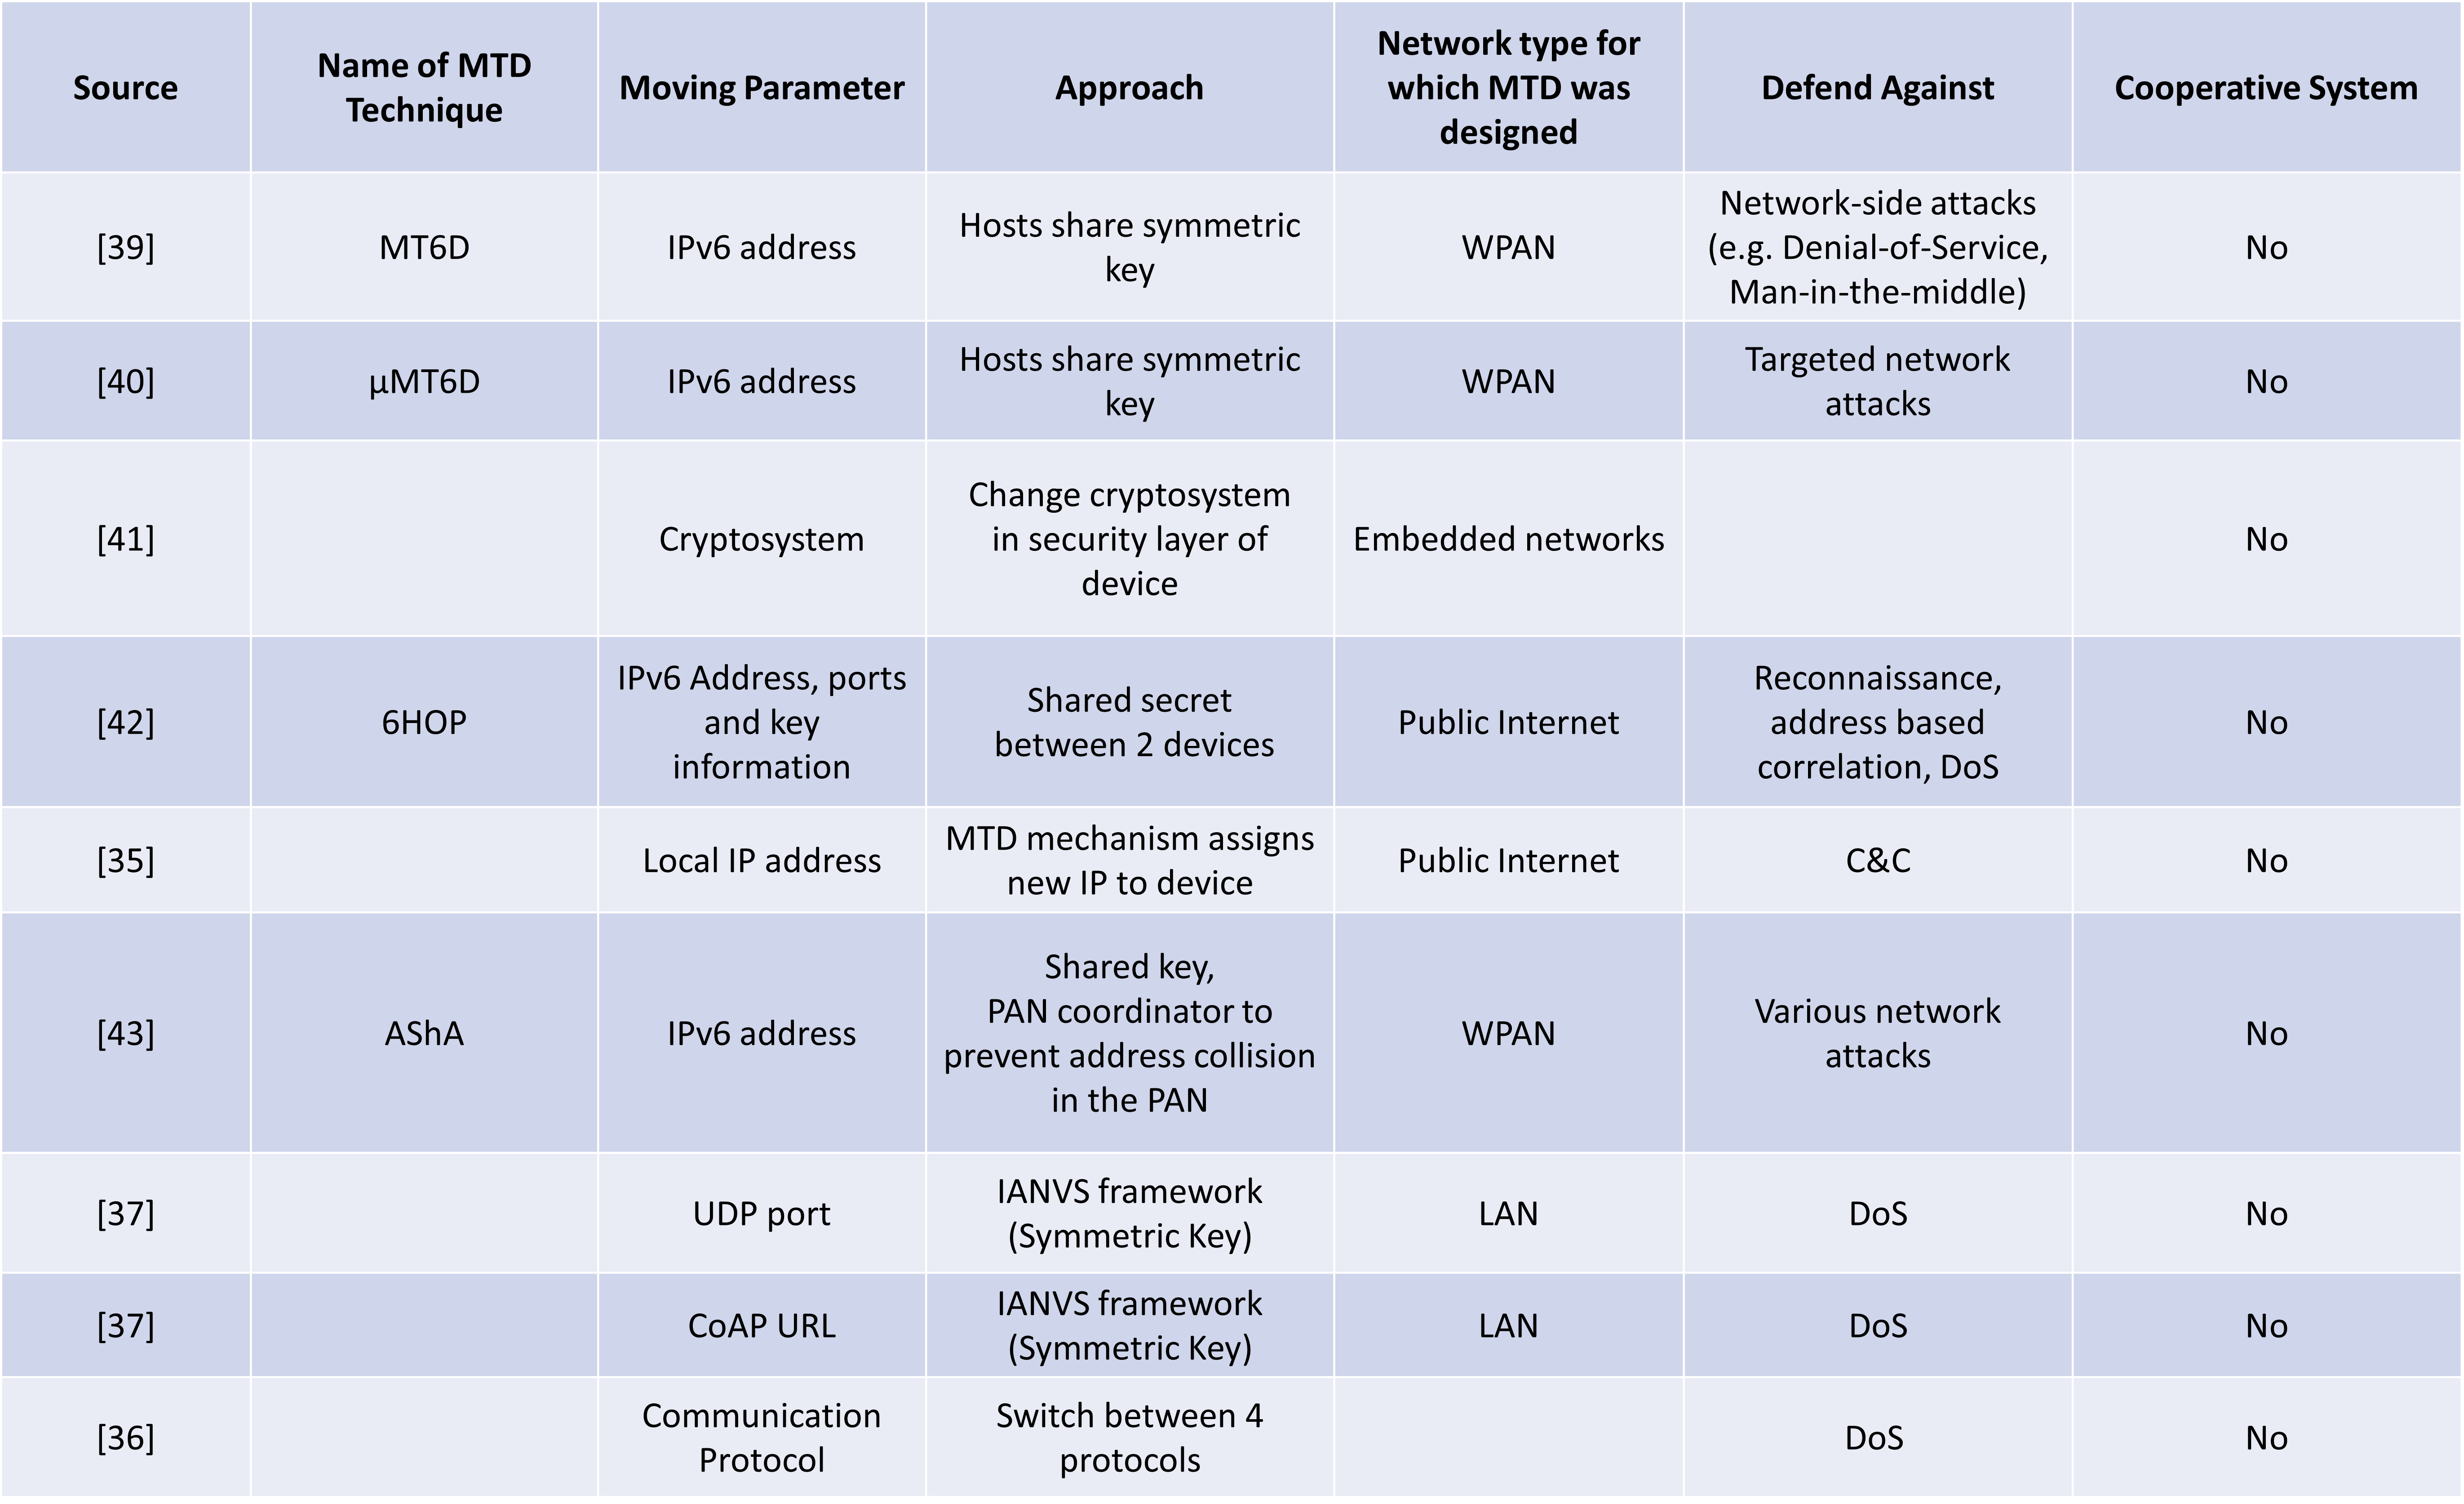
\includegraphics[scale=0.55]{assets/relatedWork.png}
\centering
\caption{A Table Summarizing Related Research.}
    \label{table:relatedWork}
\end{sidewaystable}


\chapter{Implementation}

This chapter presents the implementation details of the proposed solution, including the initial architecture created, the process of finding and modifying a suitable malware, and the explanation of the final implementation.

\section{Creating the Implementation Environment} \label{sec:prerequisites}
Before starting the implementation, a secure environment was essential, as this thesis deals with malware. To achieve this, Oracle VM VirtualBox Manager, an open source virtualisation solution~\cite{website:oracleVirtualBox}, was installed to create three virtual machines. These included a leader machine and two other VMs called VM1 and VM2. While the leader machine is used to run all the server components, the other two are intended to mimic the IoT devices. Ubuntu was chosen as the operating system as it is the most widely used operating system for constrained devices as described in Section \ref{sec:hardSoftware}. This OS had to be changed later which will be described in Section \ref{section:IssuesOfInitialPrototype}. Since the hardware details can be customized later, no further thoughts were given to this at this stage. 

Ideally, a different machine than the main computer would be used to run all the virtual machines, but unfortunately this was not an option. However, to ensure the highest level of security for the machine and the network, several security measures were taken. All the machines created were put into an internal network. This is an option within VirtualBox that creates a software-based internal network where only the machines in the network can communicate with each other. In this way, the machines cannot communicate with the host machine or the outside world, which was exactly the aim as this prevents uncontrolled spreading. A side effect was that it was not possible to download anything from the Internet. 

The solution to this problem was a shared folder that could be accessed by the host computer and the virtual machines. For additional security, the shared clipboard has been disabled and the host machine has been placed on a guest network so that there are no other devices in the same network. Therefore, even in the unlikely case of the host machine being infected, the malware could not spread across the network except to the router. However, as the default password has been changed and the latest updates are automatically installed on the router, the risk of infection is negligible. Other security measures that were already in place included a different OS on my host computer and Malwarebytes anti-virus protection. Thus, the environment created was as secure as it could be. The described environment can be seen in Figure \ref{graphic:architecture}.


\begin{figure}[h!]
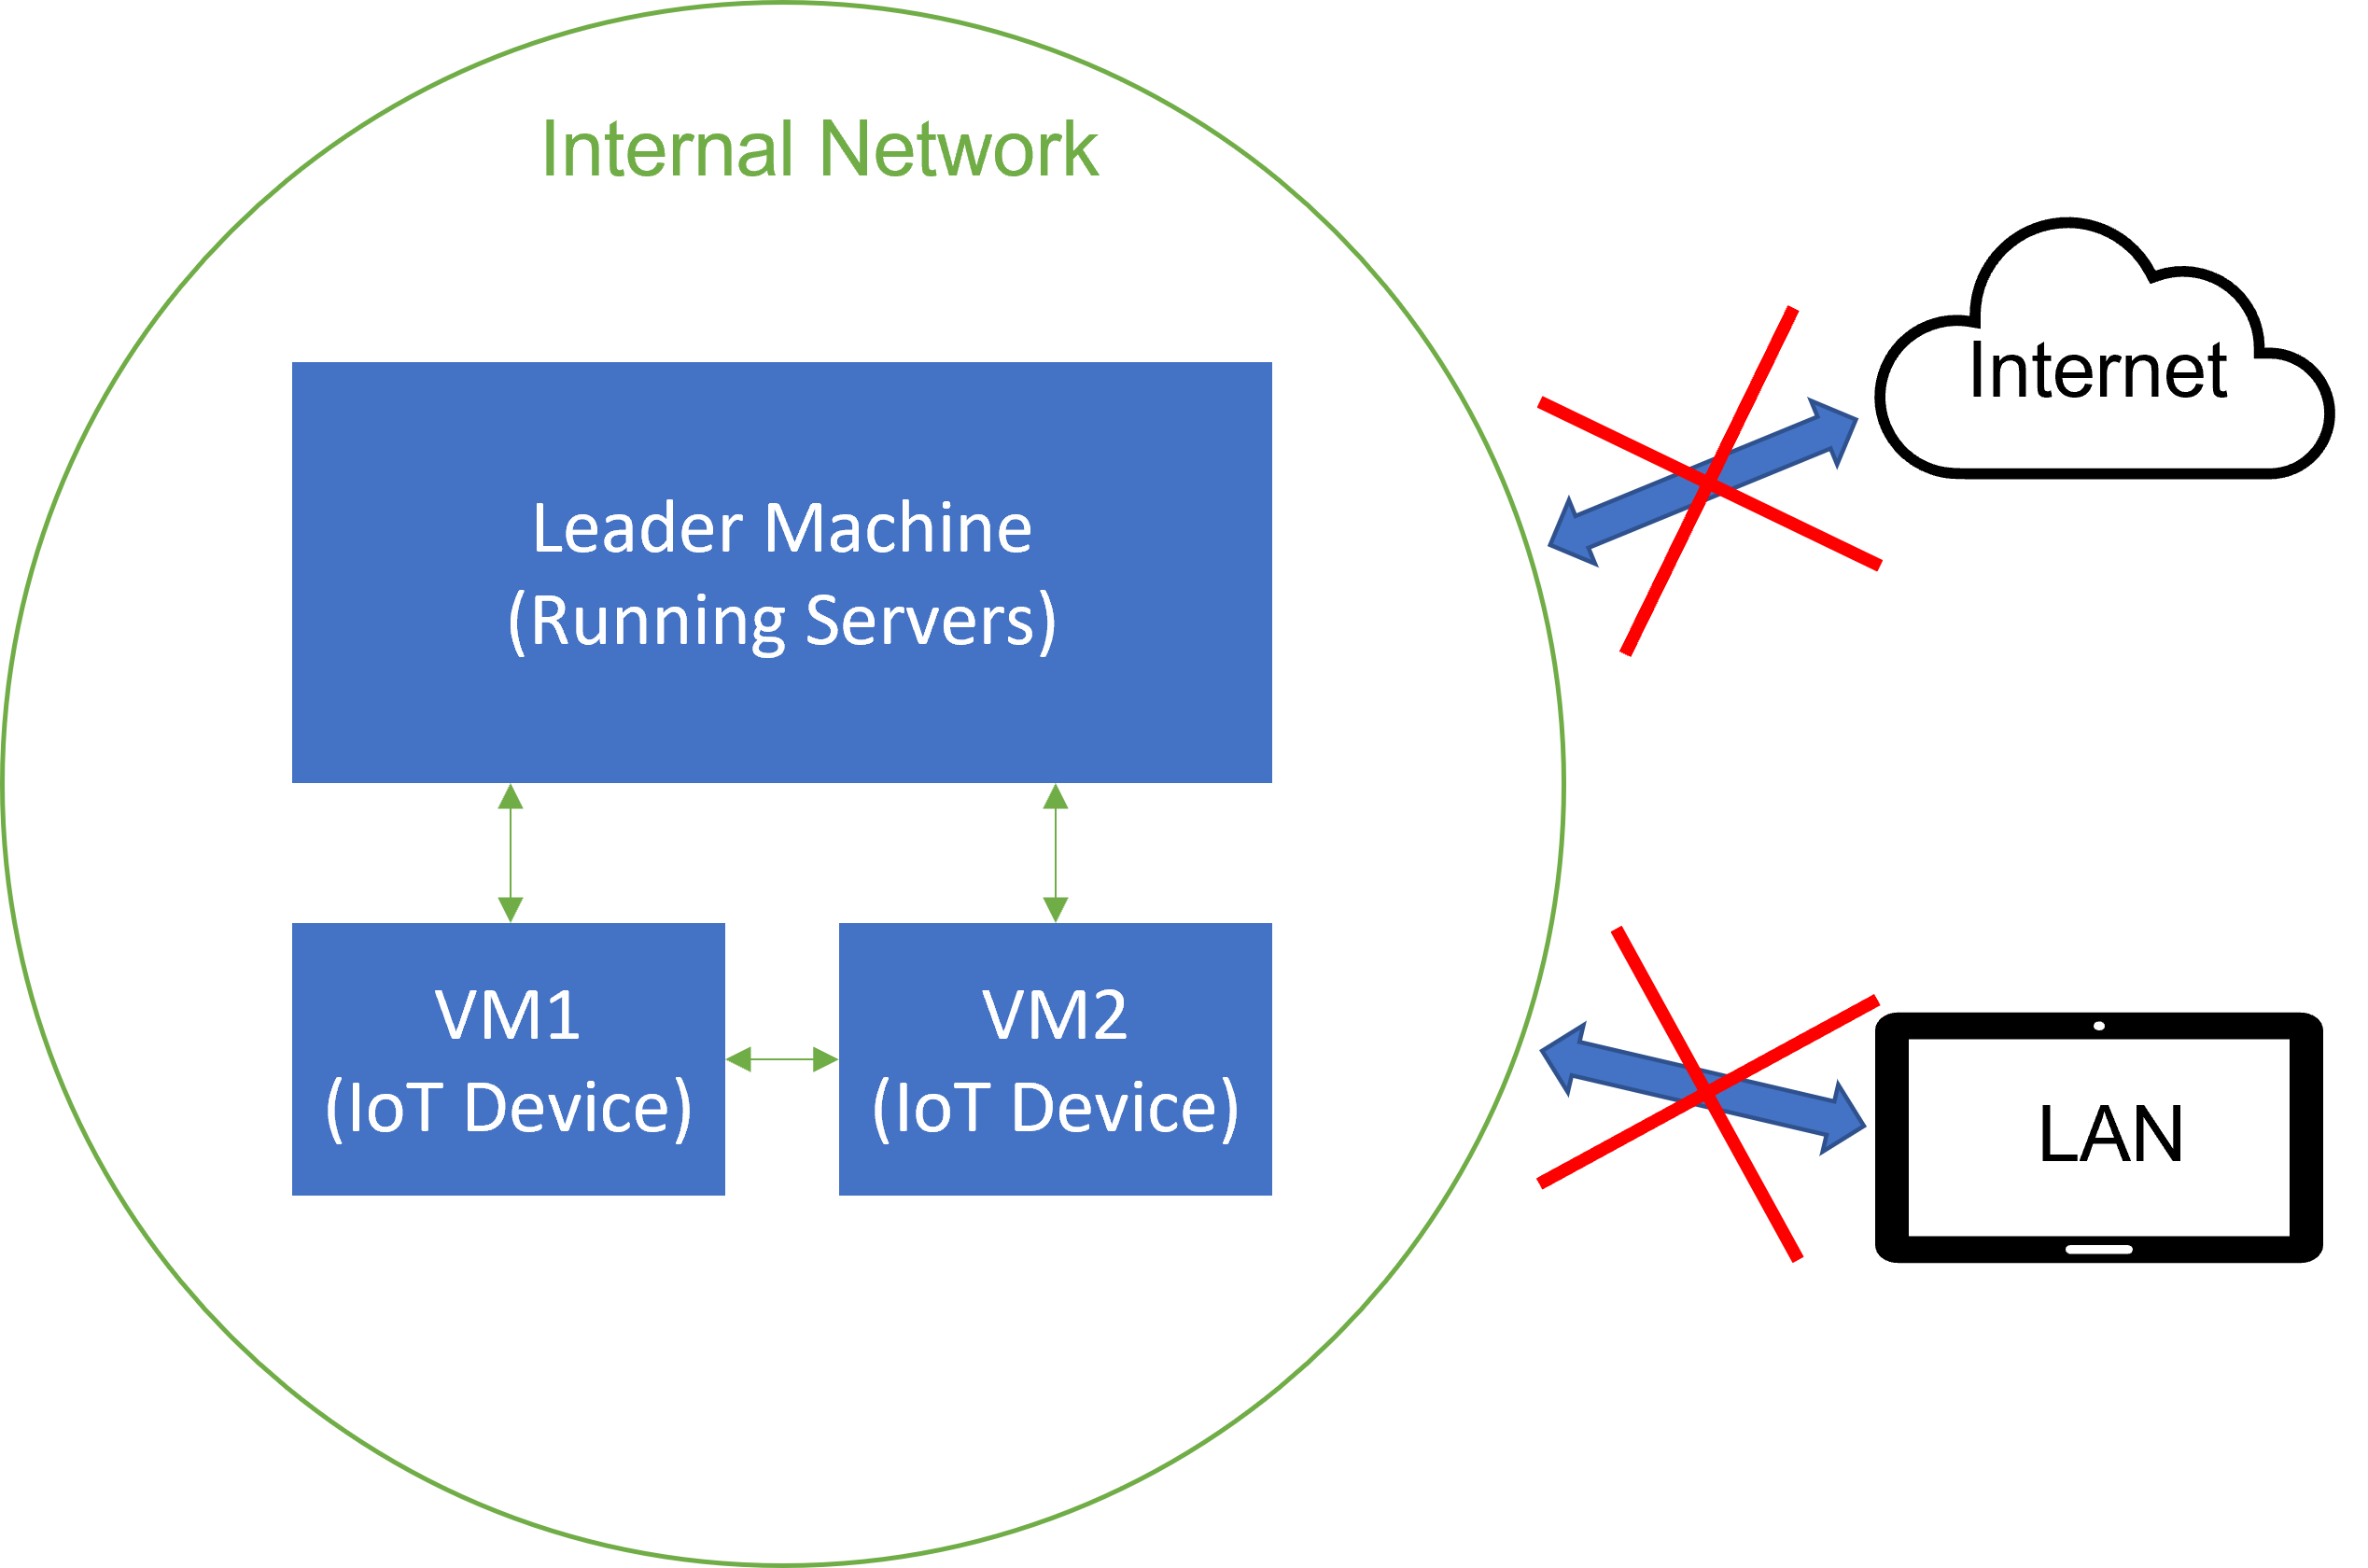
\includegraphics[scale=0.7]{assets/architecture.png}
\centering
\caption{The Created Environment With 3 Different VMs in an Internal Network Which Prevents the Malware From Spreading to Other Machines. }
    \label{graphic:architecture}
\end{figure}




\section{Initial Prototype} \label{section:initialPrototype}
The first prototype should help to better understand MTD from an implementation perspective, which should ultimately help to find appropriate solutions for the problem at hand. The architecture of this prototype was very similar to~\cite{article:Cedeno}. An overview of this architecture can be seen in Figure \ref{graphic:firstArchitecture}. The leader machine runs two applications, the \textit{MTD Deployer Client} and the \textit{MTD Deployer Server}. These two do not necessarily have to run on the same machine, but it is possible. The idea was to have these two programs do as much of the work as possible, given the hardware limitations of the IoT devices, at a later stage. The architecture is explained using the numbers in Figure \ref{graphic:firstArchitecture}.
\begin{enumerate}
    \item VM1 and VM2 continuously send information to the \textit{MTD Deployer Client}. This information consists of RAM usage and CPU usage. 
    \item The \textit{Deployer Client} continuously checks for anomalies in the information sent by VM1 and VM2. For simplicity, this anomaly is a RAM or CPU usage greater than 50\% in the last ten steps of the information sent.
    \item The \textit{Deployer Client} notifies the \textit{Deployer Server} of conspicuous behaviour in VM1 and VM2. 
    \item The \textit{MTD Deployer Server} then initiates the MTD techniques, which in this case is simply changing the private IP addresses of the virtual machines. The \textit{Deployer Server} uses the \textit{nmap} command to find all the occupied IP addresses in the network and sends each machine a new, unused IP address. 
    \item The VMs listen for commands sent by the \textit{Deployer Server} and then migrate to the newly sent IP address using the \textit{ifconfig} command. 
\end{enumerate}

\begin{figure}[tph]
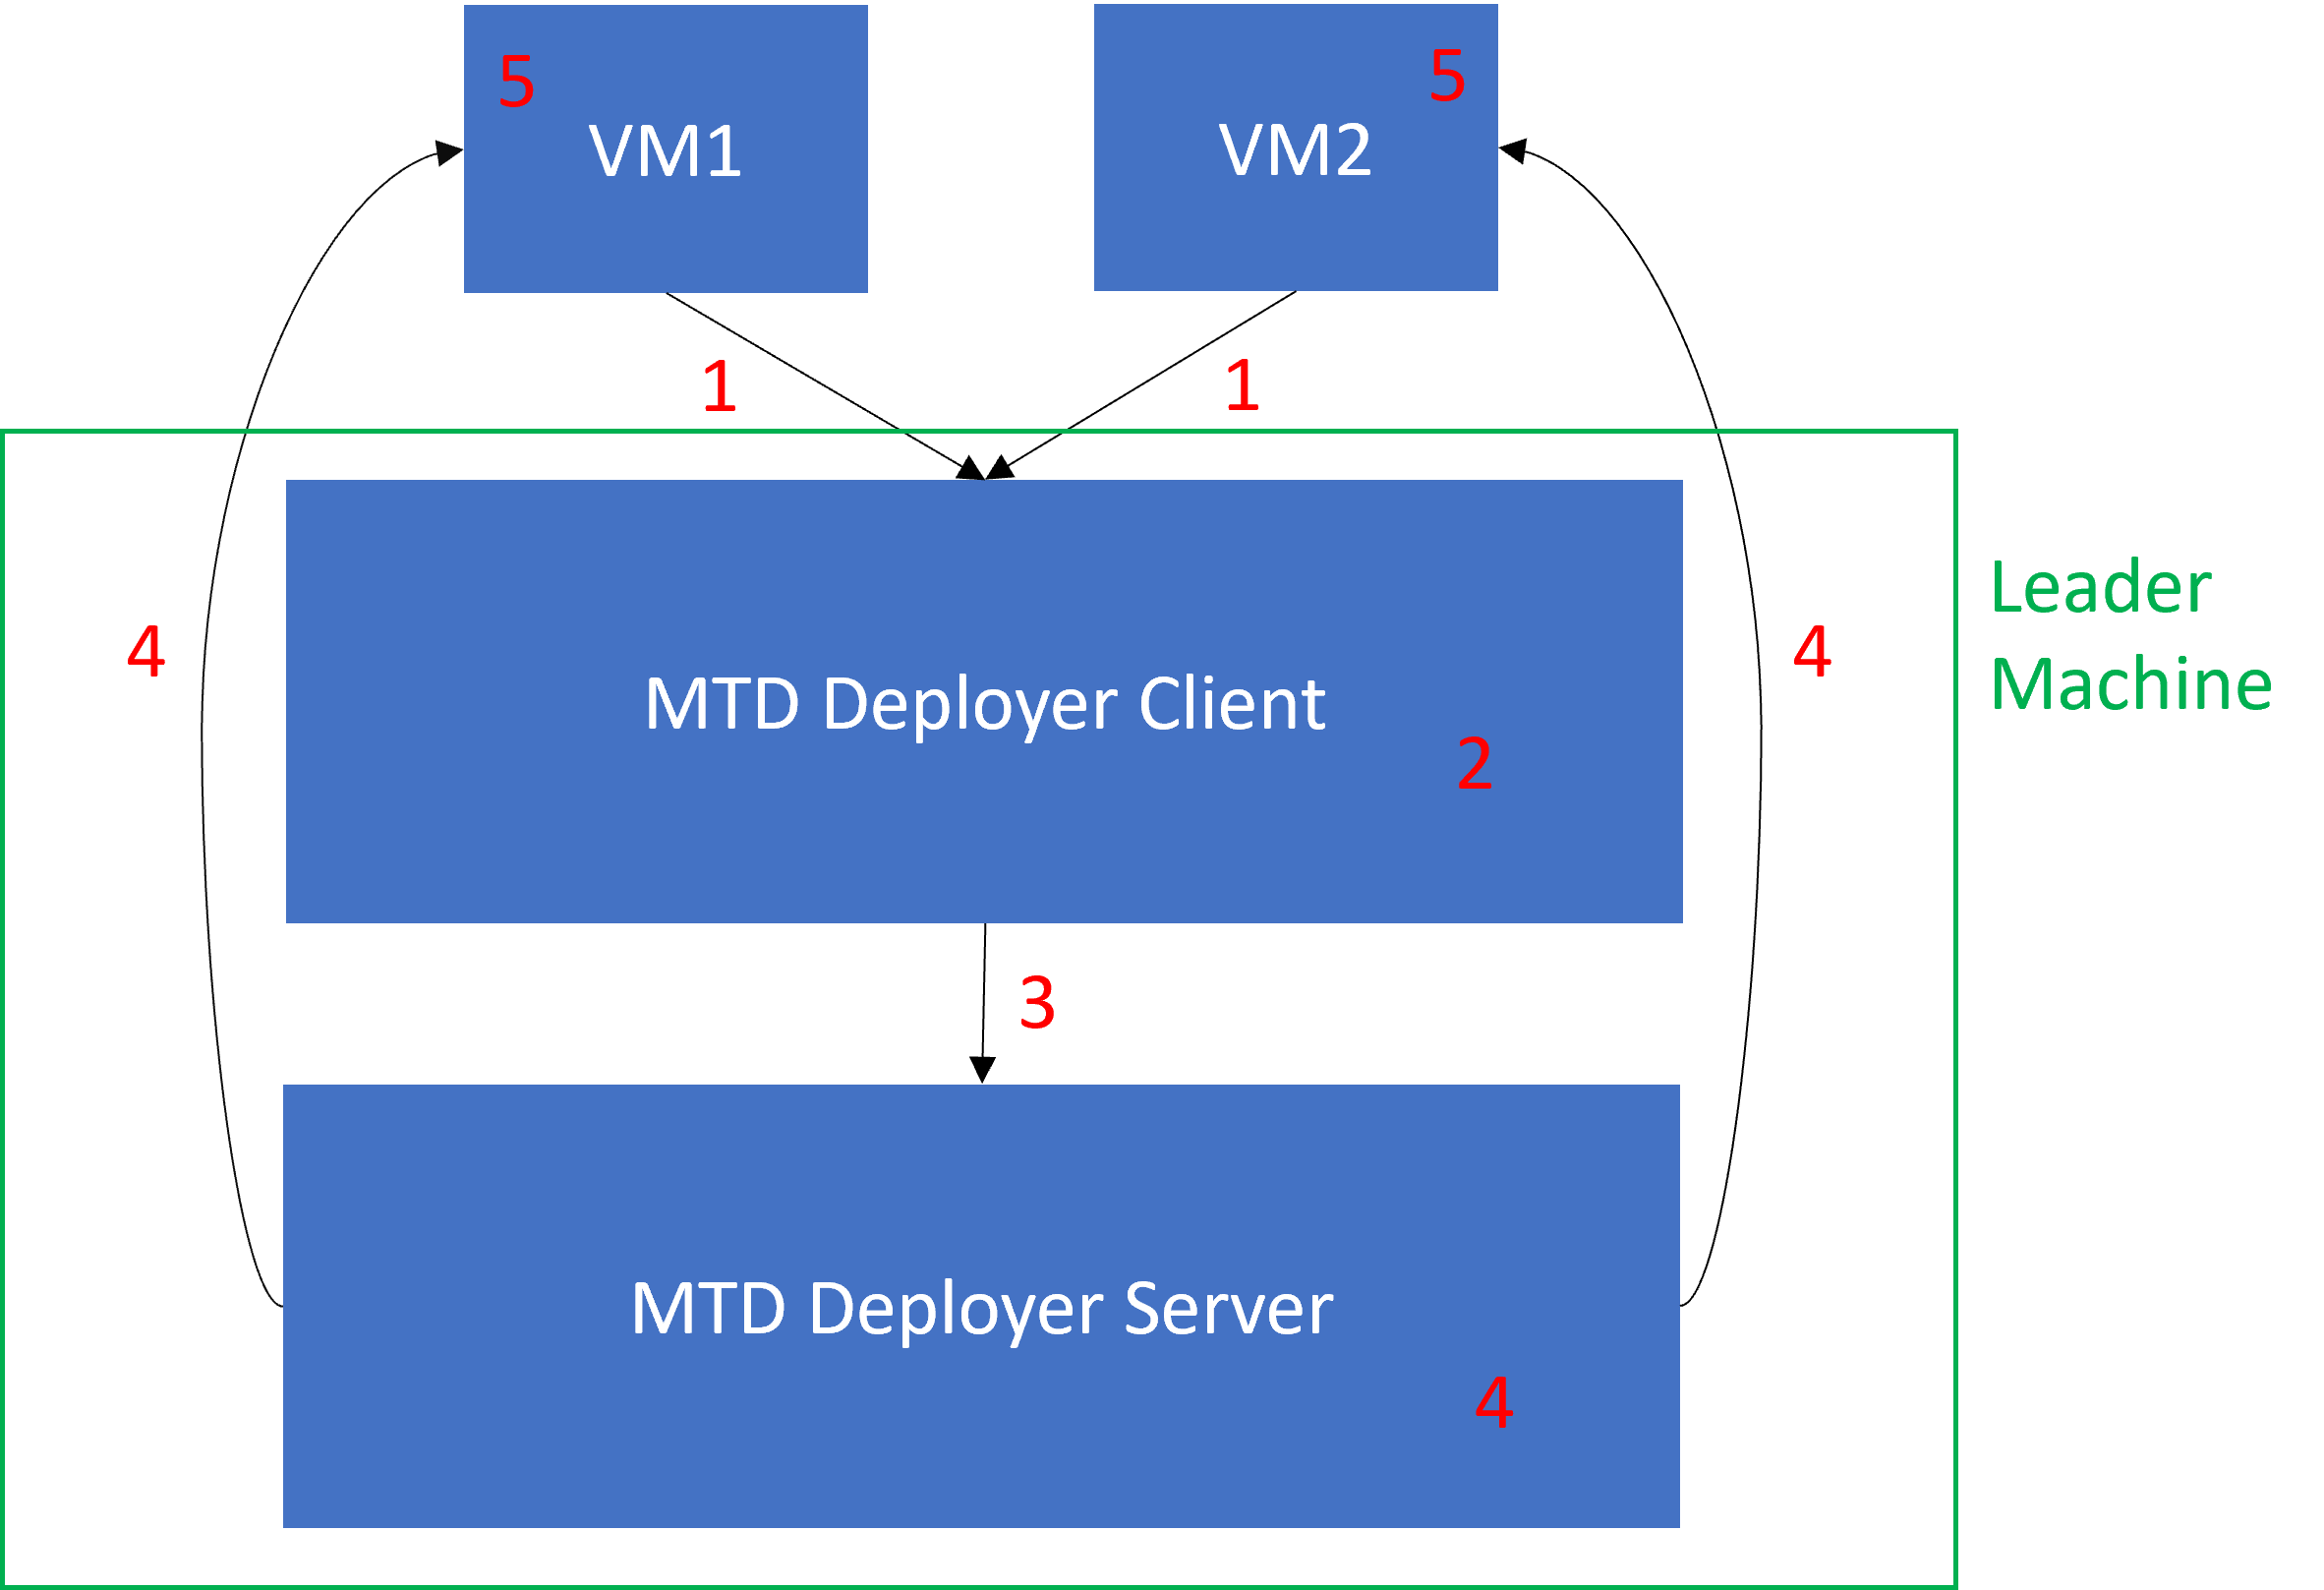
\includegraphics[scale=0.8]{assets/firstArchitecture.png}
\centering
\caption{The Architecture of the First Prototype.}
    \label{graphic:firstArchitecture}
\end{figure}

The cooperative part of this prototype is that if one VM detects malware, all VMs should initiate countermeasures, not just the affected one. This approach had several weaknesses, such as the VMs not checking that the migration to the IP address was working. This and other weaknesses were addressed in later implementations. 

This prototype was implemented in Python using sockets, which can be used to send messages across a network~\cite{website:realPythonSockets}. The prototype was also briefly tested by running all the Python scripts and manually setting the CPU usage of a VM to 100\%, whereupon the system handled the fake malware call. The \textit{Deployer Server} successfully sent messages to the VMs, which then changed their IP addresses according to the content of the messages. Thus, everything worked as expected and it was possible to continue. 


\section{Finding Malware Samples} \label{main:bashlite}
The first goal after the initial prototype was to find a suitable malware for this thesis. This was necessary for a number of reasons: Firstly, the malware had to be studied to see how it interacts with the system in order to develop the most appropriate countermeasures. This included studying the underlying code where possible. Second, it would be more meaningful to evaluate the MTD techniques with real malware. However, finding suitable malware proved to be a difficult and extremely time-consuming task. On the one hand, this was due to the rarity of malware code on platforms such as GitHub, which is understandable, as otherwise anyone could easily compile and distribute the malware. On the other hand, there were a number of requirements that the malware had to meet:
\begin{itemize}
    \item The malware should ideally target IoT devices. Although it would have been possible to use malware targeting desktop devices, the aim was to use IoT malware to get as close to the real world as possible.
    \item The malware code should ideally be openly available for study and modification. This was important as the malware will likely need to be tailored to work for this thesis. It was also important to study the code in order to find possible weaknesses in the malware.
    \item The malware had to run on the created VMs in order to execute and play with it. This was ultimately to help understand and test the weaknesses of the malware. 
    \item The malware must have a spreading functionality. This is necessary because the goal of this thesis is to use a cooperative MTD mechanism to mitigate/prevent the spreading of the malware.  
\end{itemize}

Especially the last point proved to be difficult in the end. Several code repositories such as GitHub and malware repositories such as MalwareBazaar were searched, but no suitable malware could be found. On GitHub, there exists a repository~\cite{website:iot-malware-2017} that contains the code of several IoT malware, such as Bashlite, Mirai, Lightaidra and some others. However, all of them had problems (incomplete, no spreading functionality, not executable) or were too complex to work with, as they might need to be slightly rewritten. There were other repositories, such as~\cite{website:githubMirai}, which again provided the Mirai code, or~\cite{website:githubBashlite}, which provided the same code as the first repository. The problem with MalwareBazaar was that it provided mostly executables, which was unsuitable, since code to read and modify was an essential requirement. Finally, Bashlite was chosen, even though it was initially not executable and lacked an important piece of code.

\section{Bashlite}
This section presents various aspects of Bashlite. These include the changes required to get Bashlite running, explanations of how the malware works, and an analysis of where possible MTD techniques could be applied. Note that from now on the term "client" will be used to refer to the machines that act as infected and susceptible IoT devices. This is not to be confused with the \textit{MTD Deployer Client} that runs on the leader machine and is part of the MTD framework.


The starting point was the code from~\cite{website:githubBashlite}, even though every Bashlite on Github seemed to provide the same code. Bashlite consists of two files, a server file and a client file, both written in C. Having encountered the C programming language only once in a university course and never used it again, the C language was the first obstacle, especially as the Bashlite code contained few explanatory comments. Once the general idea of the code was clear, the goal was to run it on the created VMs to see if this would work. The C files were compiled using the GNU compiler collection, which contains compilers and development tools~\cite{website:gccincredicuild} and was pre-installed on the Ubuntu systems.

Unfortunately, the execution completely failed in the case of the client script. The \textit{server.c} file was executable on the leader machine, but the client threw a fork error that was unknown to me until then. \textit{Fork} is used to create a child process, whereupon the parent and child process use separate memory spaces~\cite{website:fork}. Although several possible solutions, such as running it with \textit{sudo} or checking that the system had not reached its maximum number of processes were tried, the problem remained. After some time and a lot of trial and error, the idea came up that the underlying operating system might be the problem and not the script itself. 

Thus, new machines were set up, but this time with the Raspberry Pi Desktop OS~\cite{website:raspberryOSDesktop}. As shown in Section \ref{graphic:IoTOSs}, the Raspberry Pi OS (formerly Raspbian) had the second-largest share of all Linux distributions in IoT devices, so it is a suitable alternative. After everything was set up, the client was immediately executable on the Raspberry Pi OS. Therefore, it is not clear whether the OS was the problem in the first place, but changing it was one possible solution. Below follows a description of Bashlite's server and client and how the two files were modified for this thesis. 

\subsection{Bashlite Server}
The Bashlite server basically opens two ports on the executing machine. The first port (8888) was already defined in the code and is the port to which a "management" connects. This management then controls the server and the clients. So, to broadcast to the clients and do anything in general, one must first telnet to port 8888 of the server machine and enter a password, otherwise the server will not do anything useful with the clients. The other port opened by the server is passed as an argument when the script is started, along with the number of threads to create. The port used in this thesis was 6667, but this does not matter as long as the port is free; all that matters is that the same port is included in the client code, as this is the port to which the clients will connect after infection. The bridge between the management and the client is the broadcast function. This function takes the strings sent by the management and broadcasts them to all the clients, which then execute some commands/functions based on those strings. The important thing to note here is that no plain Bash commands can be sent directly from the management to the clients, so sending an "ls" as the management will not cause the clients to do anything. The server automatically broadcasts a "PING" to all clients every 60 seconds. Figure \ref{graphic:controlStreamServer} shows the basic control flow of the server. 

\begin{figure}[tph]
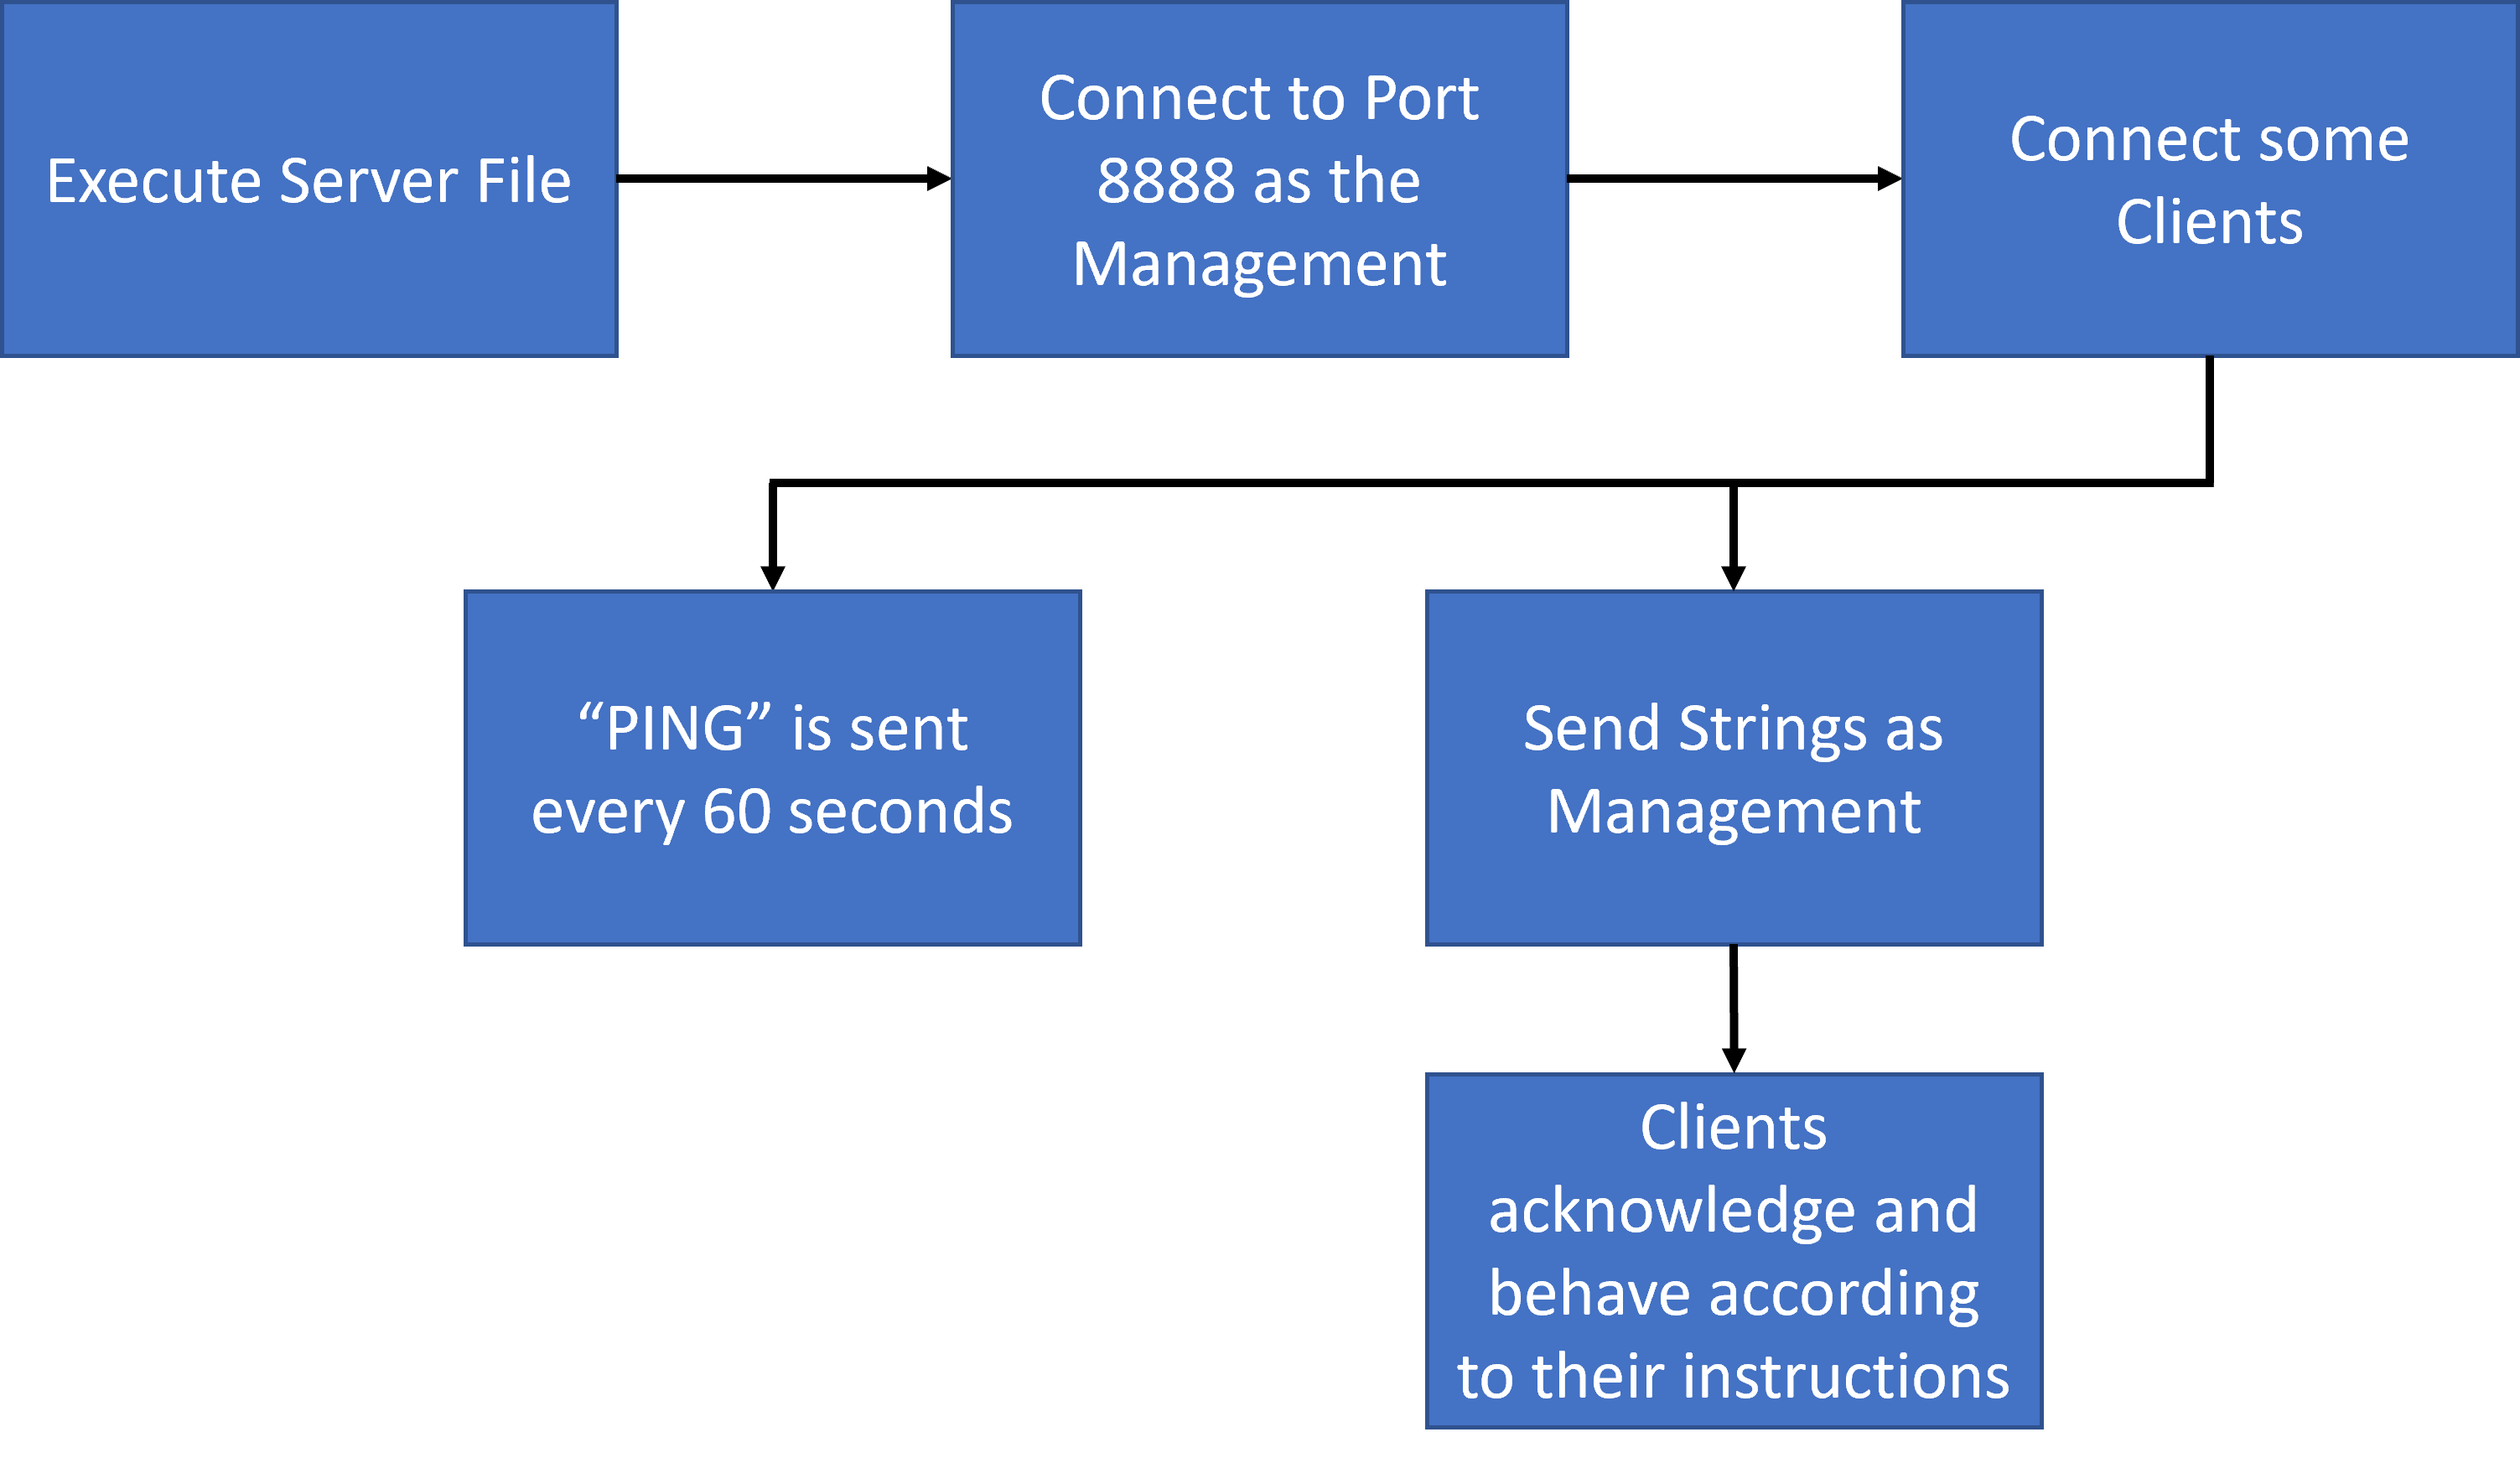
\includegraphics[scale=0.6]{assets/controlStream.png}
\centering
\caption{A Simplified Control Flow of the Server File of Bashlite.}
    \label{graphic:controlStreamServer}
\end{figure}

\subsection{Bashlite Client}
The client is much more complex than the server and contains many more lines of code. At the beginning of the client file, the IP address of the command server must be specified, and two \textit{char} arrays containing default usernames and passwords are created. Later in the code, these are used to check whether another device found is not properly secured, and if so, the correct username and password combination is stored.
Various helper functions follow (e.g. various printing options, or a function that searches for a string in the buffer), but these are not important for a rough understanding of the general concept. 

One important helper function is \textit{getRandomPublicIP()}. This function first generates a random IP address using the \textit{rand()} function, and then has a while block that basically checks if the IP address is public, and otherwise generates a new IP that is checked again, and so on. An invalid example would be if the first two octet portions of the IP address were 192.168.x.x, as this is a range for private IP addresses. Ultimately, the function returns a valid public IP address.

There are two other essential functions in the client, the \textit{processCmd()} function and the \textit{StartTheLelz()} function. The former processes strings sent by the management. The function waits for strings, whereupon the client returns a string or starts the execution of a function. Interestingly, some management strings are handled in this \textit{processCMD()} function (e.g. SCANNER commands) and some strings are handled directly in the client's \textit{main()} function (e.g. "DUP"). Some commands have to start with an exclamation mark, otherwise they would not be recognized by the client. Useful inputs were
\begin{itemize}
    \item "DUP", which terminates all client sessions
\item "!SCANNER ON" and "!SCANNER OFF", which starts and stops the \textit{StartTheLelz()} function.
    \item "!SH" \textit{arguments} which can be used to run shell commands on the clients. 
\end{itemize}

The \textit{StartTheLelz()} function is the most important and also the most complex function of the client. At the beginning of this function a struct called \textit{telstate\_t} is created. This struct contains several attributes such as an IP address, the state, the username index or the password index and is inserted into a file descriptor array (fds[]). The state attribute is essential as there are 12 different cases in this function and the state attribute determines which case the current file descriptor is in. The function starts with case 0 and then increments to the next case if all requirements in the current case are met. The following paragraph briefly describes the main tasks of each case. 

Case 0 checks if it is theoretically possible to connect to an IP returned by \textit{getRandomPublicIP()}, and also increments the index of the username and password if the current file descriptor was sent back by Case 3 or 5. Case 1 checks for timeouts and the like. Case 2 checks if a login is requested by the connected IP address, Case 3 sends the username and also resets the file descriptor to Case 0 if the username was wrong, otherwise it sets the state to 4. Case 4 checks if a password is requested, Case 5 sends the current password of the file descriptor, and Case 6 checks if the password is correct and resets the file descriptor to Case 0 if not. Case 7 checks if the shell is accessible and Case 8 checks if Busybox is installed. Case 9 either sends a report to the server or continues with the subsequent cases which were not needed. The simple report sent to the server is just a string in the format "REPORT IPaddress:username:password". 
Figure \ref{graphic:flowChartClient} shows the process of the client in a simplified flowchart. 


\begin{figure}[tph]
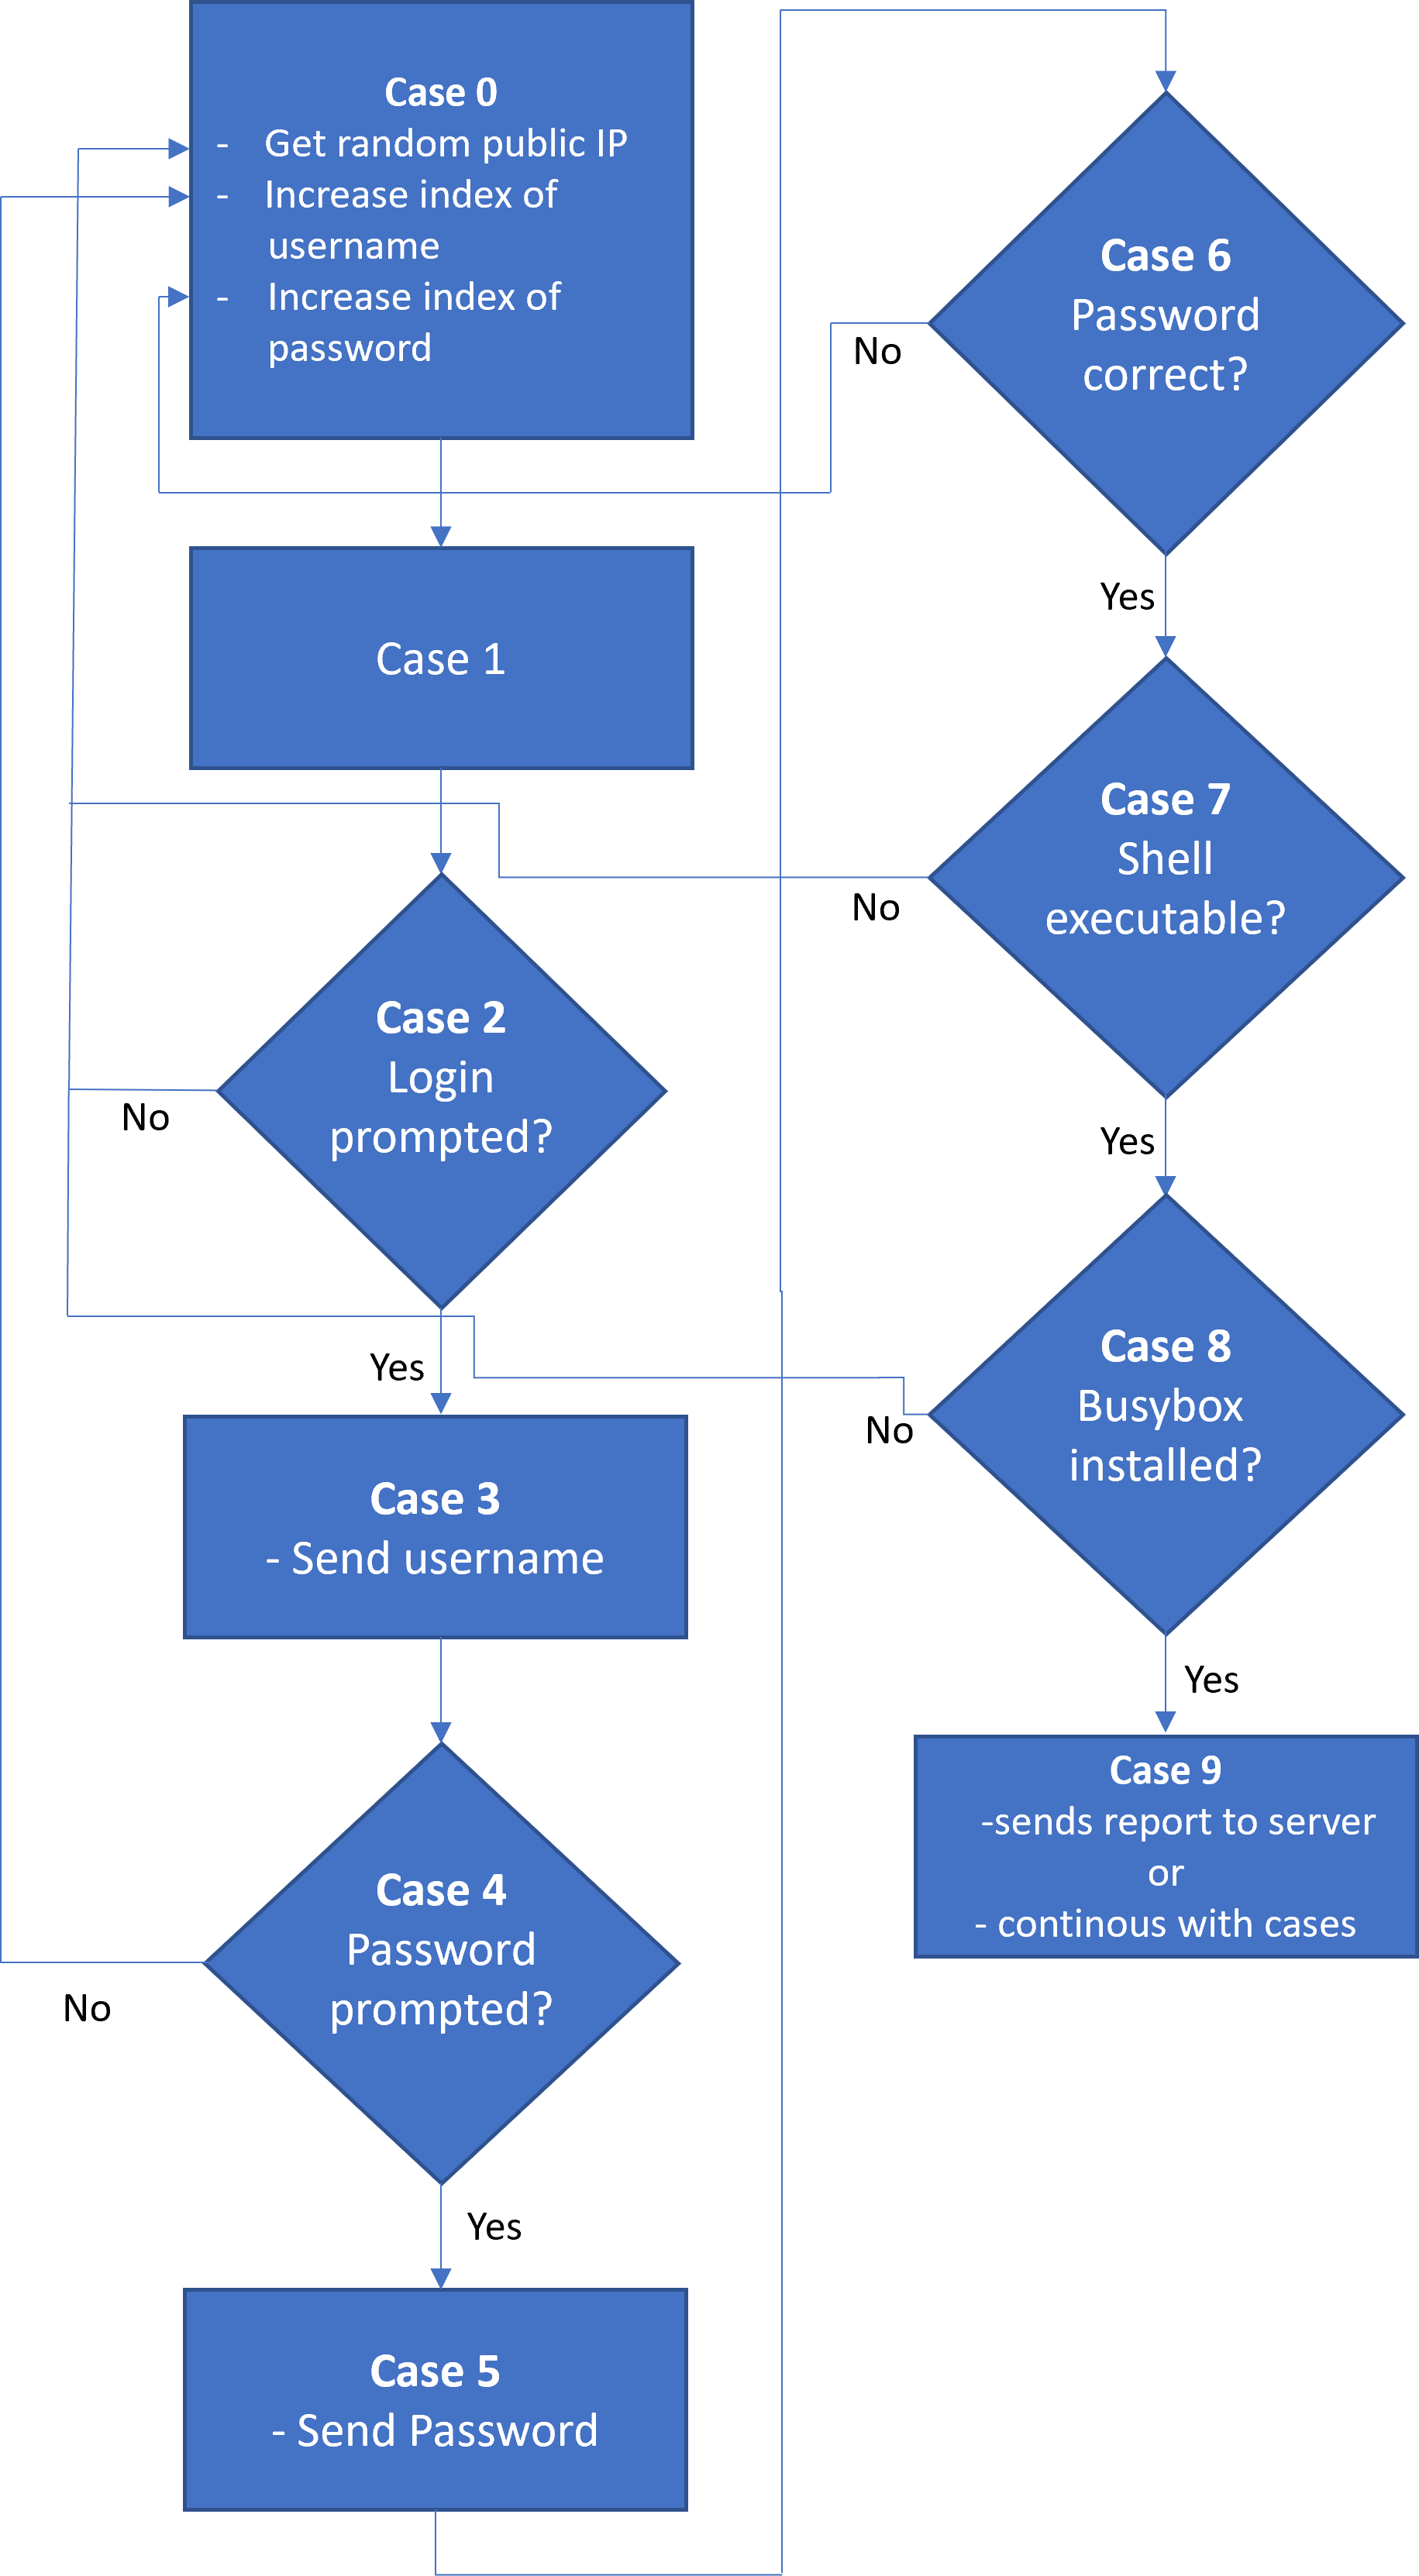
\includegraphics[scale=0.8]{assets/flowChartClient.png}
\centering
\caption{A Simplified Flow Chart of the Bashlite Client's Essential 	\textit{startTheLelz()} Function, Which Searches for Other Susceptible Devices. The Incoming Arrows to Case 0 Directly Point to the Action That Will be Executed.}
    \label{graphic:flowChartClient}
\end{figure}


\subsection{Code Modifications}
In order to get Bashlite to work as it is supposed to, several parts of the code had to be modified. This subsection describes those changes. The client was simpler to modify, probably because the code was intended to run as it was from the start.
In addition to many print statements to make the code understandable, the first step was to adapt the IP address of the command server and the arrays of usernames and passwords. Since the username and password of the susceptible machine are known, the corresponding combination was put into these arrays and the rest was deleted. Additionally, the script initializes another variable called "stillRunLelz". This variable was necessary because when the scanner on the first machine resumed scanning after sending the report to the server, the server often had trouble recognising that a second machine was now connected. So a workaround was to run the outermost while loop of the \textit{startTheLelz()} function for as long as "stillRunLelz" was 1, and after another vulnerable machine was sent to the server, "stillRunLelz" was set to 0 and the scanner stopped. This would certainly not be an applicable solution in a real malware, but it was sufficient for this thesis, as one additional infected machine was enough to test the concept.

The \textit{getRandomPublicIP()} function was also modified to return the IP address of the susceptible machine directly. Again, this would not make sense in real malware, but it sped up the development process without compromising the quality. Another problem was that the code never got further than case 6. This was solved by investigating where it failed and then sending it directly to case 7. Case 9 also checked a condition that was somehow not met, but this was solved by ignoring the condition and simply sending the report to the server at the beginning of case 9. These were all changes that had to be made to get the client to work so that a report of the vulnerable machine was sent to the server.



The server was more complex to adapt because some of the code was missing. Again, the first step was to add print statements to get a deeper understanding of how the server works. The second step was to add the missing code. This involved code to automatically exploit the IP address with the information sent by the client's scanner. To develop this, a separate C file was created so that Bashlite would not have to be continuously restarted. The code in this new file splits the report string into substrings to separate the IP address, username and password. The C function \textit{strtok()} with ":" as delimiter helped to achieve this. The rest was more complex, as the server still had to automatically connect to the susceptible machine, copy the client file to that machine, and run the client file. The best way to do this was with a Bash script called from the \textit{server.c} file with the \textit{system} call. The first attempt of a Bash script using Telnet for the connection failed, probably due to the back and forth interaction between the two machines. The next attempt was an \textit{expect} script. These scripts talk to other programs, know what to expect from them and give them the corresponding response~\cite{website:linuxExpect}. 

The \textit{expect} script starts with a timeout command of 30 seconds, so that it would not run for too long if it somehow failed. After that, the script creates variables for the arguments that are passed when the script is called. The call must be made in the following way:

\[ \mbox{telnetConnection.except \textit{IPAddress} \textit{username} \textit{password} \textit{fileToSend}}  \]

The first three arguments are given by the report string, the last one was a convenience in case a different file was to be sent to the client. The next step was to spawn the telnet command with the \textit{IPAddress} argument, whereupon the script expected the string "raspberry login:" and then sent the \textit{username} argument. This pattern continued until the \textit{expect} script connected to the susceptible machine via Telnet. The script then needed to copy the client file from the server machine to the susceptible machine. This copying functionality was important because it could have provided another defence option at a later stage. Since installing additional packages or creating an ssh key or password was not an option, the options to transfer the file were limited. This brought \textit{netcat} into focus, as it provided a good way to transfer the client file~\cite{website:netcat}.

Thus, the susceptible machine should open a \textit{netcat} connection on a port and then wait for the server to send the file over that connection. This worked perfectly when typed directly into Bash from both the client and the server, but it became more complicated than anticipated in the \textit{expect} script due to two constraints. The first was that the client obviously had to open a connection before anything could be sent from the server, and the second was that it was somehow impossible to send the files from the \textit{expect} script on the local machine. 

There were considerations to take the sending of the files out of the \textit{expect} script (and have it done by another script), but this was not practical. The reason for this was that the \textit{expect} script would then have to run partially (until it opened the \textit{netcat} connection on the susceptible machine), then pause until the client file was sent by another script, and then continue running the rest of the \textit{expect} script. The solution to this problem was to swap the server and client \textit{netcat} tasks. Previously, the vulnerable machine would open a connection and wait for the file to be sent from the server machine. Now the server machine opens a port to send the corresponding file and waits for the susceptible machine to request it. This made it possible to first run the \textit{netcat} command on the server and then start the \textit{expect} script in the same \textit{system()} call in C as the \textit{expect} script requested the file from the server.
Additionally, the content of the client file had to be pipped into \textit{netcat} on the server side, otherwise the transfer would fail. The final command can be seen in Algorithm \ref{lst:Pseudocode openNetcatStartExpect.py}.
\\


\begin{lstlisting}[caption={The Bash Command Used to Open a Netcat Connection From the Server to Send the File Once the Client Requested it and to Start the \textit{Expect} Script},label={lst:Pseudocode openNetcatStartExpect.py}]
cat fileToSend | netcat -q 5 -l 9899 & expect telnetConnection.expect IPAddress username password
\end{lstlisting}

Algorithm \ref{expectPseudocode} shows the \textit{expect} script in pseudocode. Now everything worked and experiments with MTD techniques and malware spreading were possible.
\\

\begin{lstlisting}[caption={The \textit{Expect} Script in Pseudocode},label={expectPseudocode}]
SET timeout 30
SET IPaddress to argument 0
SET username to argument 1
SET password to argument 2
SET fileToSend to argument 3
CONNECT to IPaddress with telnet
EXPECT "raspberry login"
SEND username variable
EXPECT "password"
SEND password variable
SEND netcat command to request the file
SEND sleep for 7 seconds
SEND command to make the requested file executable
EXPECT "password for"
SEND password variable
SEND sleep for 3 seconds
SEND execute client file
EXIT expect script
\end{lstlisting}


\subsection{Analysis of Bashlite} \label{analysisOfBashlite}
This section presents an analysis of Bashlite. This includes possible levers where MTD techniques could be applied to mitigate Bashlite.

 
As part of the analysis of Bashlite, many timing properties had to be checked. This required selecting suitable hardware properties for the VMs as a first step. As described in Section \ref{sec:prerequisites}, the hardware details were not a concern initially. To simulate a Raspberry Pi device, hardware similar to that used by~\cite{article:vonderAssen} was used, consisting of a 1.5 GHz CPU and 3.7 GB of RAM. The device running the VMs is a Surface Book 1 with 16 GB of RAM and an Intel Core i7-6600U dual-core CPU running at between 2.60 GHz and 3.40 GHz~\cite{website:intelInfo}. In VirtualBox it is possible to specify how many cores a VM can use and also the execution cap for those cores. Unfortunately, it is not possible to simply give the VM a frequency for its processor (e.g. 1.5 GHz). Thus, the performance information provided by the Windwows task manager had to be used as a reference to calculate the required execution cap. The task manager indicated that the laptop's base speed is 2.81 GHz. This appeared to be correct on average (even with all VMs running). Thus, each infected VM was given one core and an execution cap of 53\%, because 53\% of 2.81 GHz is about 1.5 GHz. In addition, the virtual machines have 3.7 GB RAM allocated to them by VirtualBox.


An infection process of Bashlite can be divided into four different phases, which are presented below. 
\begin{enumerate}
\item The first phase is when the infected client scans for susceptible devices and sends the information to the Bashlite server.
\item The second phase is when the server receives the report from an infected device and initializes the Telnet connection to the susceptible client. The duration of this phase is extremely short.
\item The third phase begins as soon as the Telnet connection to a susceptible device is started.
\item The fourth phase begins when the Bashlite client is launched on the susceptible machine.
\end{enumerate}


The first important data to get was the number of seconds these Bashlite phases took to complete. It is important to note that this could be different for a more sophisticated/varied malware or much better hardware on the devices, but Bashlite could serve as a reference. To achieve this, Bashlite was run 10 times and the time was measured by hand. Due to the various scripts on the server side, it was too complex to measure the time programmatically, so it was faster to do it manually. Other reasons were that it was not necessary to know the exact times and that the phases always took about the same number of seconds. The only time a script measured the execution time was in phase 2, as this period is too short to measure by hand. For phase 1, all time values were between 14 and 17 seconds, with an average of 15.5 seconds. Phase 2 lasted an average of 0.00007 seconds, making it negligible. Phase 3 time values ranged from 60 to 63 seconds with an average of 62 seconds. Thus, on average, 62 seconds pass before the susceptible machine is infected. The long duration of phase 3 is due to the \textit{expect} script written to connect, fetch the client file from the Bashlite server and execute it. This \textit{expect} script needed several sleeps to complete the actions, and the Telnet connection also takes some time. Perhaps the whole script could be written differently, but this was not possible without putting too much effort in it. 
Figure \ref{graphic:timelinePhases} shows the corresponding timeline, where phase 2 and 3 have been combined and the phases are colour-coded according to whether or not it is still possible to mitigate the spreading to the second device. 


\begin{figure}[tph]
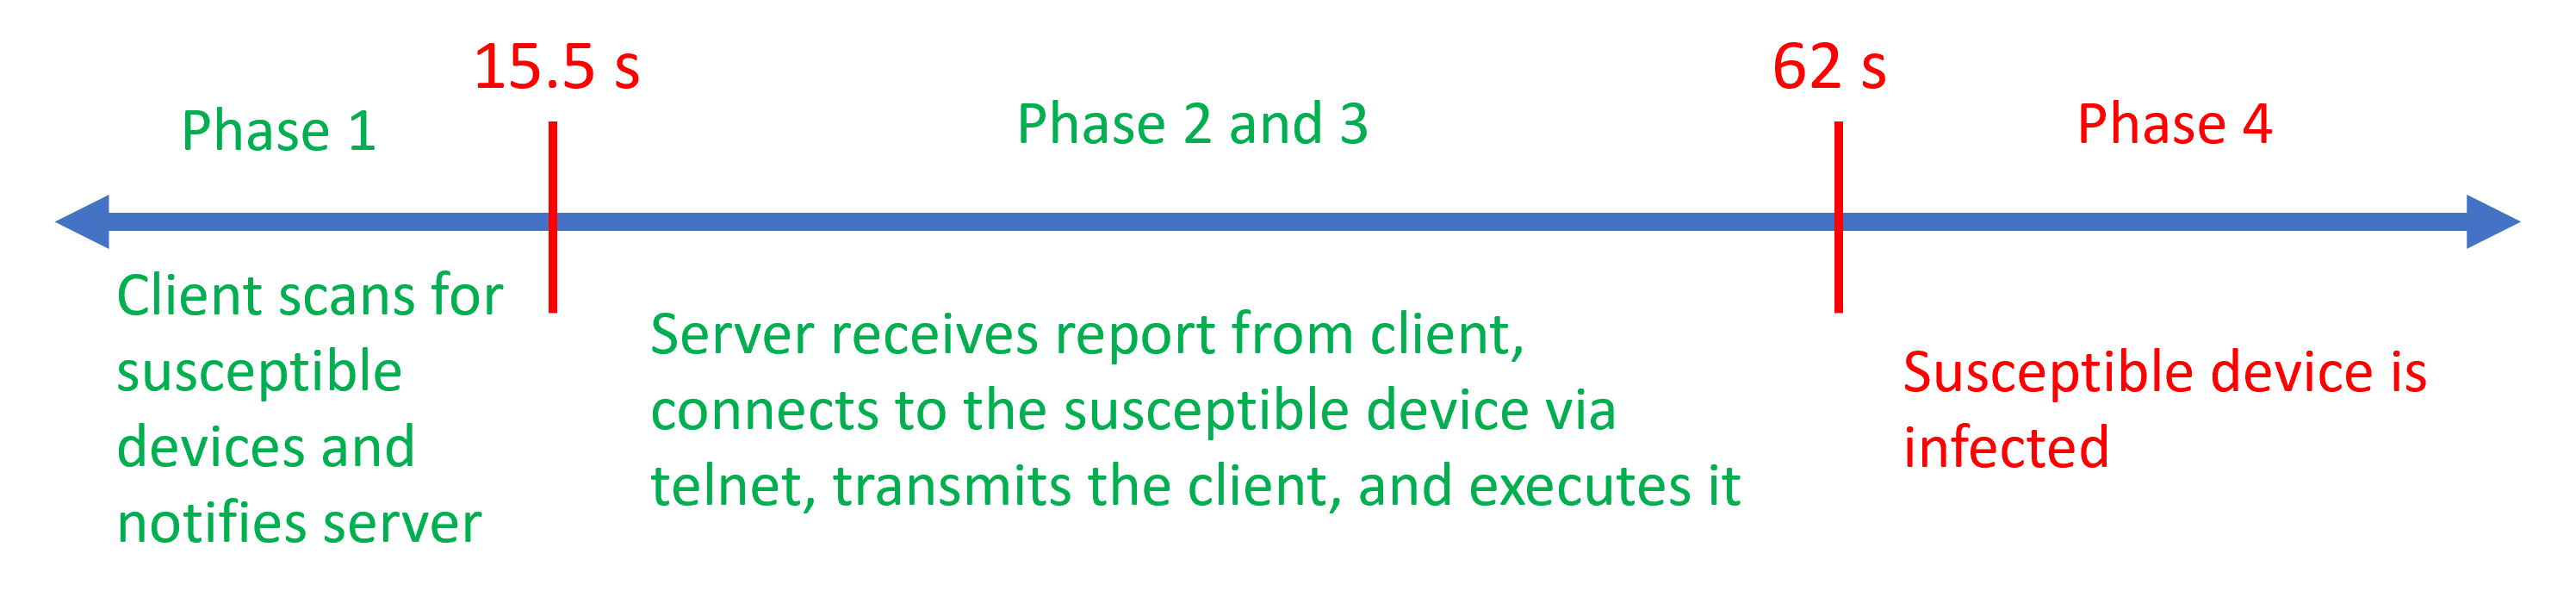
\includegraphics[scale=0.7]{assets/timelinePhases.png}
\centering
\caption{The Timeline Showing the Different Phases of a Bashlite Infection of one Susceptible Device.}
    \label{graphic:timelinePhases}
\end{figure}


%This allowed me to assess whether the proposed MTD techniques would also work against Mirai without running it. Even though there is a big difference in the code, it is obvious that Mirai's scanner also targets telnet ports, specifically port 23 and port 2323. The latter is often used as an alternative for port 23~\cite{website:gitSpeedGuide}. So it is safe to say that MTD techniques targeting these ports should work, at least in theory, for Mirai as well. The same holds for the "HEH" malware presented in Section \ref{subsection:P2PIoTBotnets}, as this malware also uses port 23 and port 2323 to infect devices~\cite{website:trendMicroUncleanable}. Even though I focus on Bashlite's characteristics below, MTD techniques that target ports 23 and 2323 should also be able to mitigate the spreading of Mirai and HEH. I will return to this in the evaluation. 
%\todo{see if the ip change also woud work for mirai}

%In addition to Bashlite, a part of the section deals with Mirai~\cite{website:githubMirai}. Even though Mirai is too complex to examine in detail in a short period of time, I compared Mirai's scanner file to the one of Bashlite to see, if they share the same weaknesses. 





%es chan jo au sii, dass de virus no anderi sache macht wie nur mitem command server verbindet, drum macht sinn wenn men scho vorher unterbindet

\section{Final Implementation} \label{section:finalImplementation}
This chapter presents the final implementation based on the analysis of Bashlite in Section \ref{analysisOfBashlite}. The implementation is based on the same structure in terms of VMs as the initial prototype in Section \ref{section:initialPrototype}. Again, the structure consists of three different virtual machines. The first is a leader machine running two applications, the \textit{MTD Deployer Client} and the \textit{MTD Deployer Server}. Both applications consist of two Python files, one of which acts as a listening socket, while the other contains the essential helper functions for the listening socket. For example, the \textit{MTD Deployer Server} has a listening Python file called \textit{listenToDeployerClient.py} and a \textit{sendToDevices.py} that sends the MTD execution commands to the devices.

The other two machines are the clients that mimic the IoT devices and also consist of two files each. The \textit{sendToDeployerClient.py} notifies the \textit{Deployer Client} when malware has been found, and the \textit{listenToDeployerServer.py} executes the corresponding MTD technique using the information sent by the \textit{sendToDevices.py}.
Even though this chapter briefly explains every file, the focus lies on \textit{sendToDevices.py} (\textit{Deployer Server}) and \textit{listenToDeployerServer.py} (client), as these two form the basis of the MTD techniques. However, before explaining the code, this section first introduces the chosen MTD techniques and how they relate to the background information from Section \ref{section:background}. 

\subsection{Implemented MTD Techniques} \label{section:implementedMTDTechniques}
The analysis of Bashlite described in Section \ref{analysisOfBashlite}, together with the working implementation of Bashlite described in Section \ref{main:bashlite}, provided the opportunity to search for suitable MTD techniques. These techniques should ideally protect against classic botnets and P2P IoT botnets. The first subsection below describes the implemented MTD techniques based on the analysis of Bashlite in Section \ref{analysisOfBashlite}, and the second subsection theoretically evaluates how these MTD techniques against Bashlite could protect against Mirai and HEH.


\subsubsection{Implemented MTD Techniques Based on the Analysis of Bashlite}
The first phase of Bashlite ends with the report sent from the infected client to the Bashlite server.~\cite{article:vonderAssen} and further experiments in this thesis have shown that it is possible to disrupt the connection between the Bashlite client and the Bashlite server by changing the IP address of the client. If the connection is disrupted before phase 2 begins, the report can be prevented from being sent, resulting in the best possible mitigation case. Once the second phase begins, the IP address change of the originally infected machine (VM1) will have no effect on the spreading of Bashlite to the susceptible machine (VM2). Of course, the IP address change should still be executed to disconnect the infected machine from the server, but this has no advantage in terms of spreading to the susceptible machine (VM2). This makes the second technique all the more important. The idea of this second technique is to move the Telnet port of the susceptible machines for some time while Bashlite is rendered harmless on the infected machine. This essentially hides the susceptible machines from the infected machine's scanner. 

This Telnet service port change technique works in phase 1. As just described, this prevents the infected machine's scanner from finding the susceptible machines. This technique theoretically also works in phase 2, although it is unlikely that the Telnet service port change is applied at this point because phase 2 is so short. The port change also works in phase 3, but it requires a small adjustment because once the connection between a susceptible machine and the Bashlite server is established, the port change has no effect. Thus, a potential Telnet connection must first be killed, and then the port changes must be applied to ensure that this susceptible machine is completely unreachable to a Bashlite scanner. In phase 4, the second machine is already infected, but the Telnet service port change should still be applied to all other machines in the network, as it could protect other, not yet infected machines (which were not present in the setup). Figure \ref{graphic:timeline} graphically shows the MTD techniques in combination with the phases. Note that the colours only indicate whether the applied MTD technique can prevent Bashlite from spreading to the susceptible machine. So a red font does not mean that the technique should not be applied, but that it has no effect on the Bashlite infection of other machines in the network. A green font means that the Bashlite spreading can be completely mitigated, a yellow font means that the spreading to the susceptible machine could not be mitigated, but the port change could still help other machines in the network. 

\begin{figure}[tph]
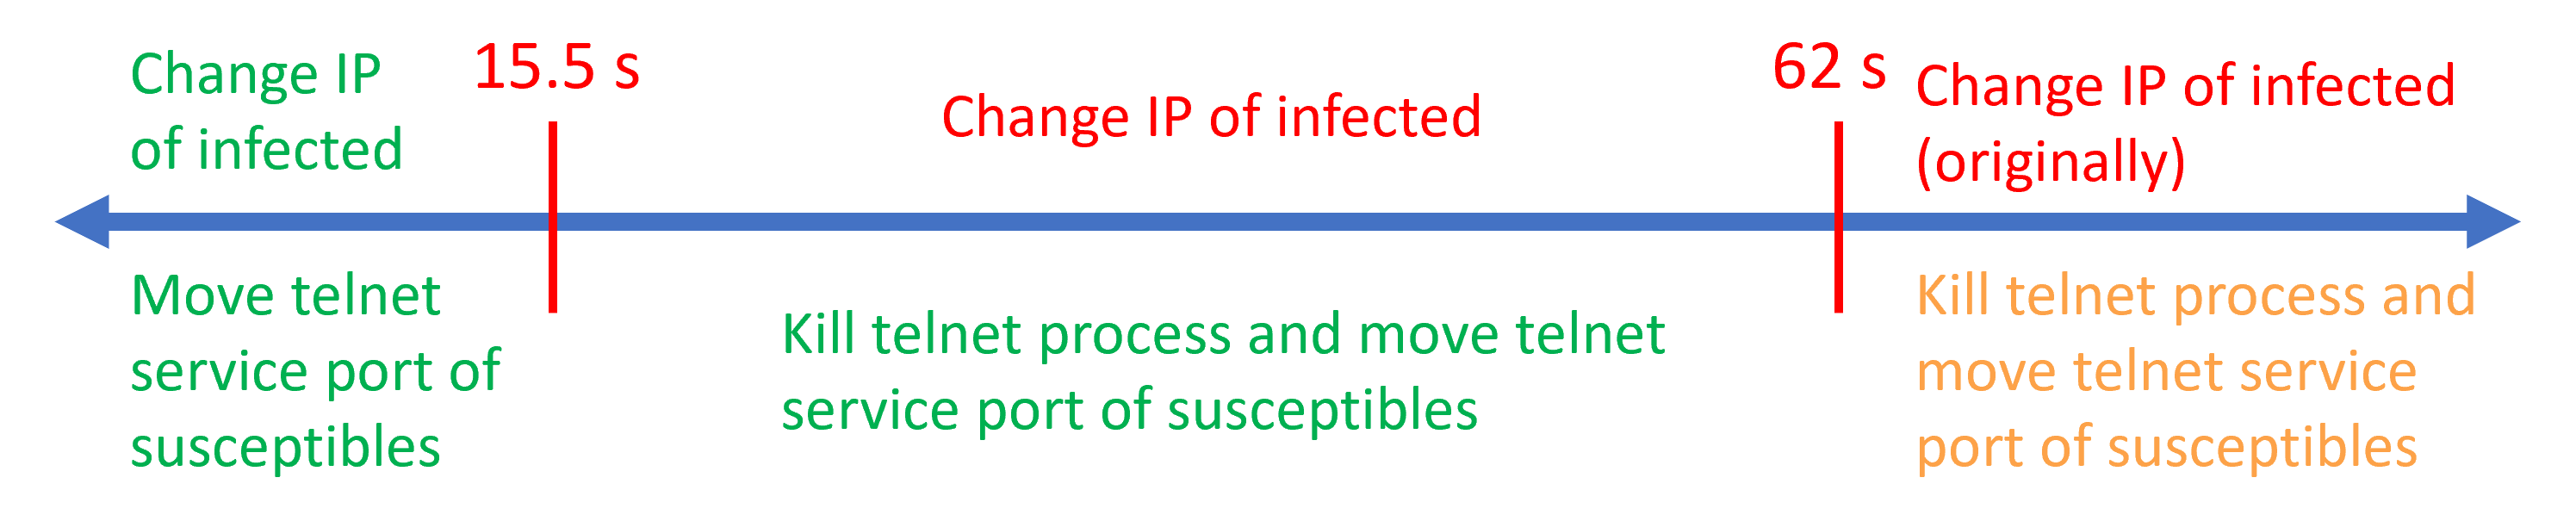
\includegraphics[scale=0.7]{assets/timeline.png}
\centering
\caption{The Timeline of an Infection With Bashlite of a Susceptible Device, Showing When the Mitigation is Still Possible.}
    \label{graphic:timeline}
\end{figure}

\subsubsection{Theoretical Evaluation of MTD Techniques Against Mirai and HEH}
A quick examination of Mirai's scanner file allowed an assessment of whether the proposed MTD techniques would work against Mirai without running it. Although there is a big difference in the code, it is obvious that Mirai's scanner also targets Telnet ports, specifically port 23 and port 2323. The latter is often used as an alternative for port 23~\cite{website:gitSpeedGuide}. The same holds for the HEH malware presented in Section \ref{subsection:P2PIoTBotnets}, as this malware also uses port 23 and port 2323 to infect devices~\cite{website:trendMicroUncleanable}. It is therefore safe to say that MTD techniques protecting port 23 (2323) should also work against Mirai and HEH, at least in theory. This is not the case for the IP address change. Although it is not possible to test it in the scope of this thesis, Mirai has a teardown functionality that is triggered when no response is received from the C\&C server. After this teardown, the client simply reconnects to the C\&C server, making the IP address change only a temporary obstacle. As for the HEH malware, it is not possible to predict the impact of the IP address change due to the unavailability of the code. However, as these types of botnets are extremely dangerous by nature, it is all the more important to prevent them from spreading. Changing the Telnet service port can therefore be considered an essential tool against all three malware types.

Once the required MTD techniques had been chosen, they needed to be defined according to the background information given in Section \ref{section:background}. This chapter introduced the three elements that define MTD techniques~\cite{article:Cai}. These three elements are "what", "how" and "when" and are used to formally describe the solution below. 

\subsubsection{Formal Definition of the Applied MTD Techniques}
The "what" to move is the IP address value and the port value of the Telnet service. The domain from which these two values are taken is defined in a configuration file, so that the user can choose in which range the value of the moving parameter should be. Of course, any IP address or port already occupied in the network or on the machine is automatically removed from this domain.  
The "how" is completely random. A random IP address or port value that is within the specified range but not yet in use will be used to replace the current moving parameter value. The final element is the "when" to move. As Bashlite has been shown to be detectable~\cite{article:vonderAssen}, the proposed solution uses an event-based decision process that includes a proactive and a reactive component. The IP address change technique is the reactive component, as it reacts to the detection of Bashlite and then initiates the countermeasures. In a sense, the port change is both reactive and proactive. Although it is also triggered by the detection of Bashlite (reactive), it also acts as a proactive component on the uninfected machines, as the technique attempts to get ahead of a Bashlite infection. The information just described can be seen graphically in Table \ref{graphic:tableAppliedMTDTechniques}.

\begin{table}[tph]
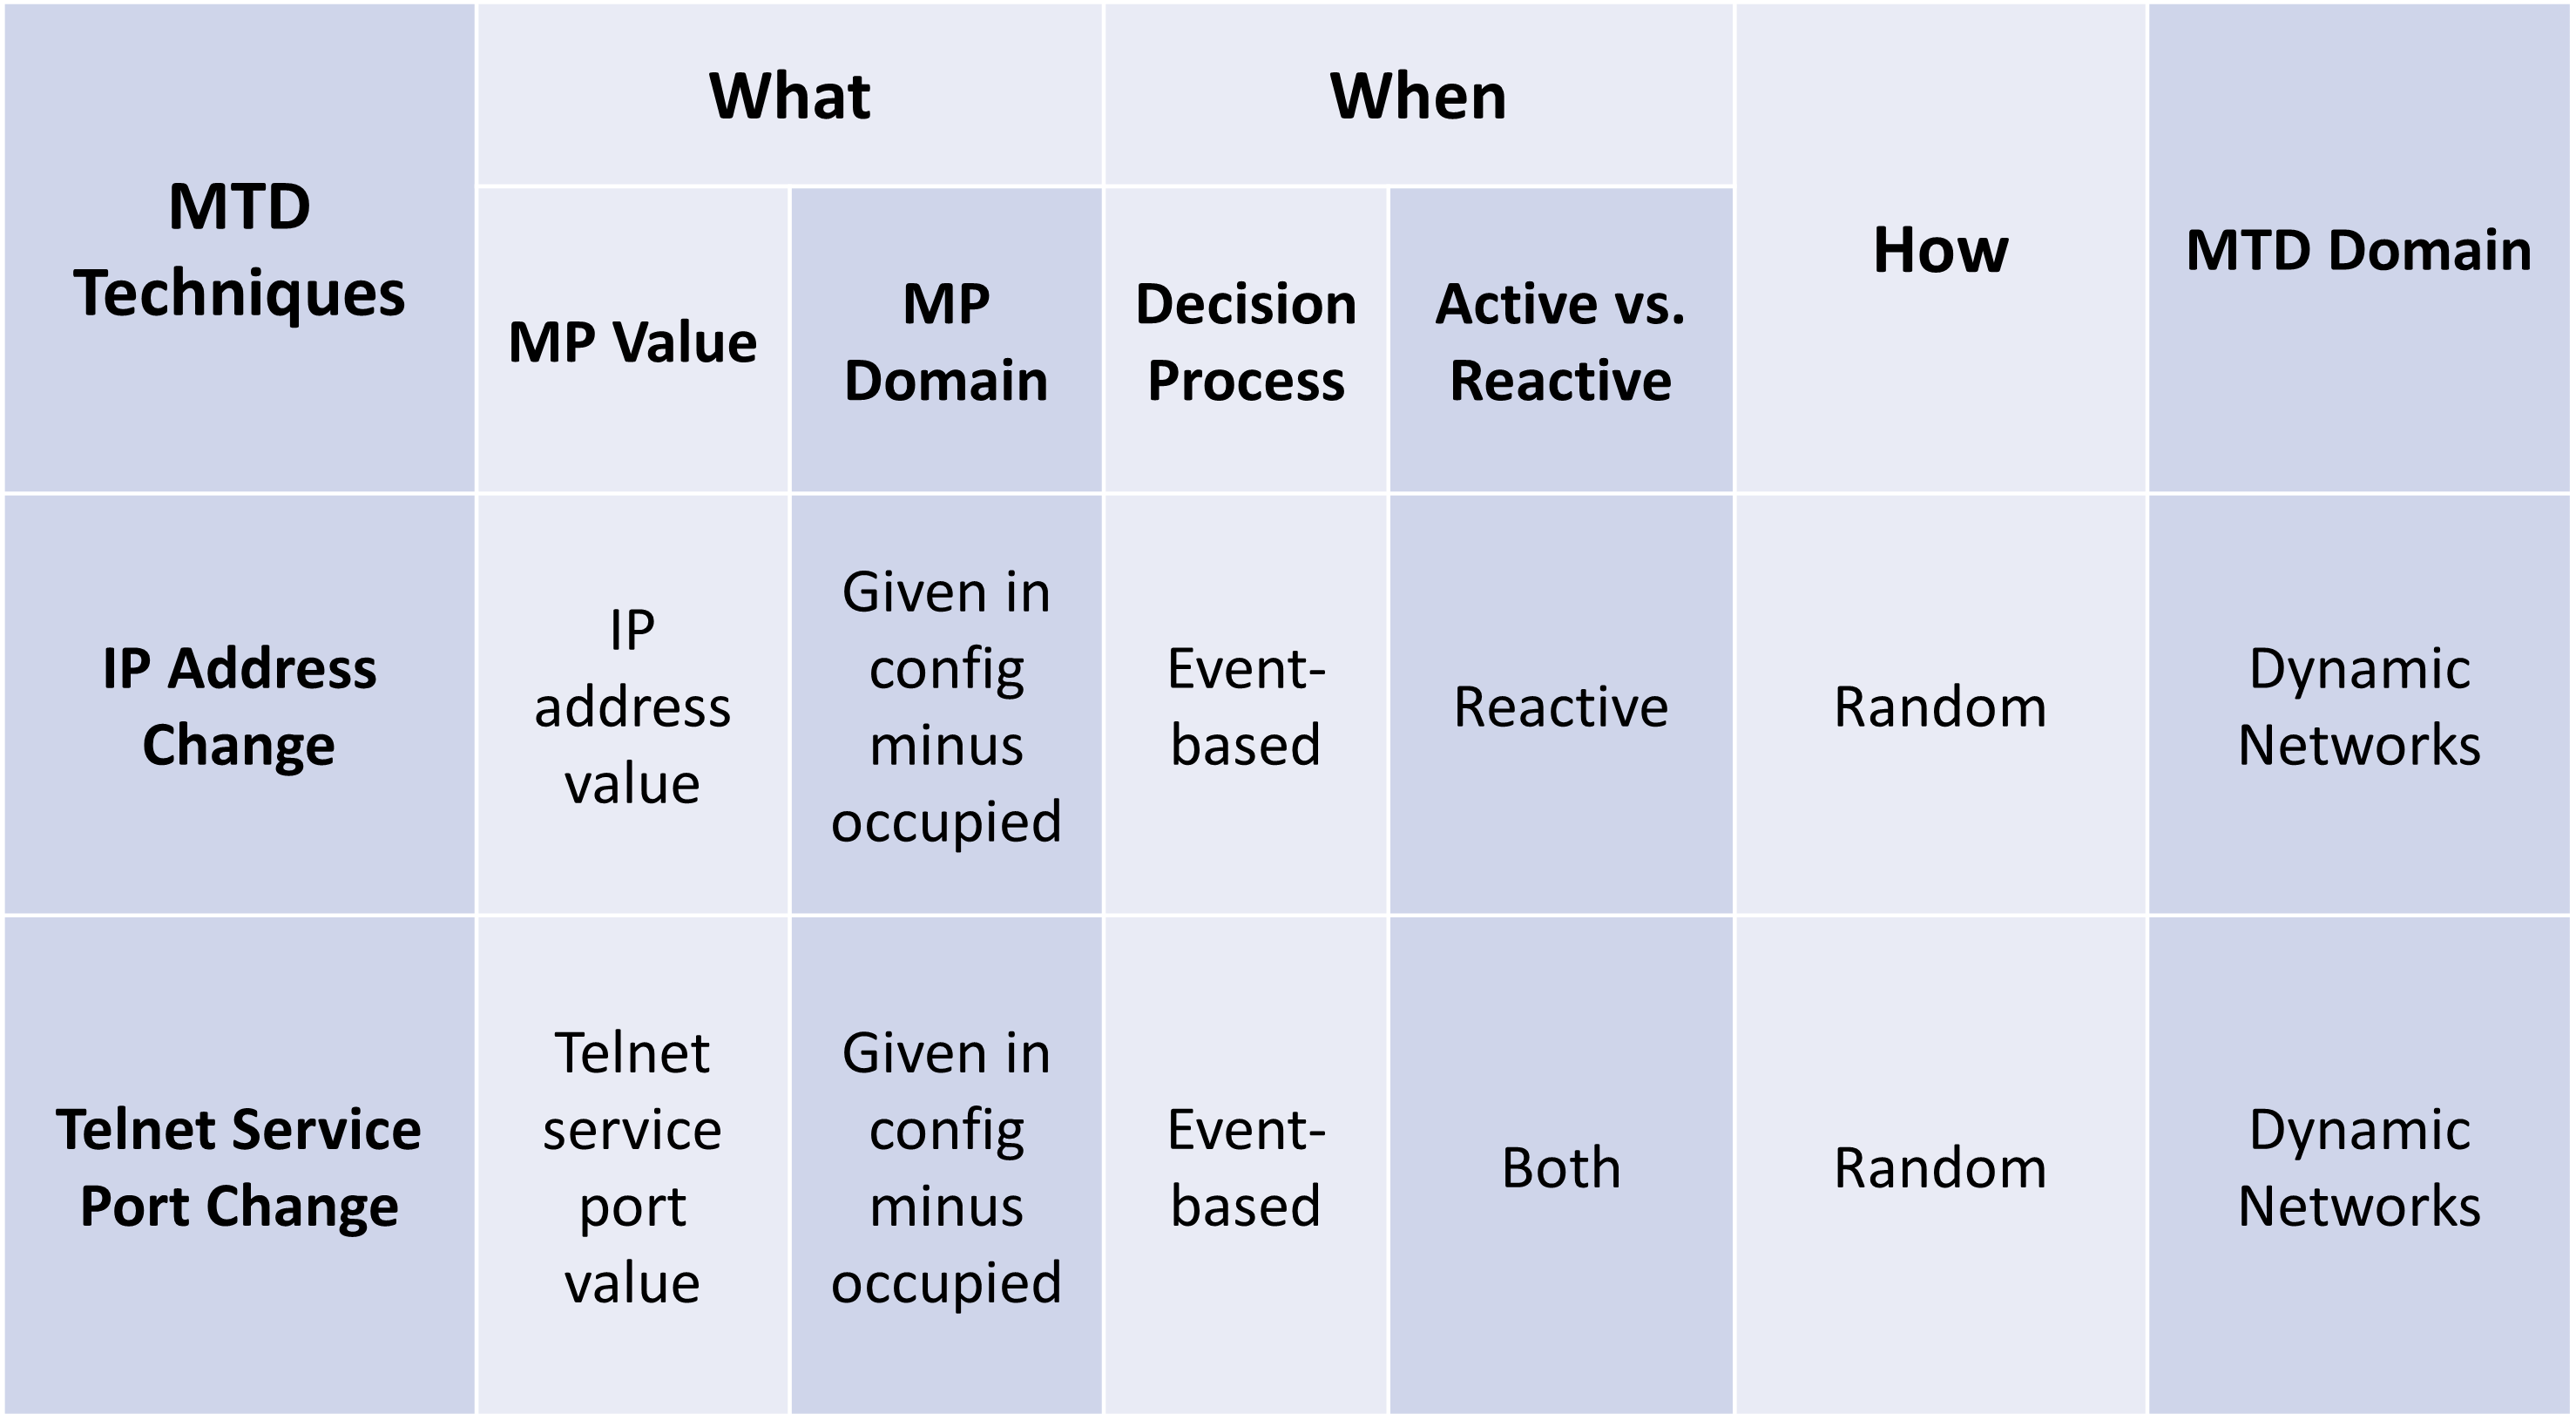
\includegraphics[scale=0.7]{assets/tableAppliedMTDTechniques.png}
\centering
\caption{A Summary of the MTD Techniques Applied With Respect to the Three Fundamental Elements of IoT Techniques.}
    \label{graphic:tableAppliedMTDTechniques}
\end{table}



Although both MTD techniques clearly fall into the dynamic network category, the classification of the attack phase they seek to disrupt is not as straightforward as~\cite{article:okhraviFindingFocus} indicated. The reason for this is that I consider the five-phase attack of~\cite{article:okhraviFindingFocus} to be more applicable when an attacker has a specific target to attack. Bashlite aims to infect as many generic devices as possible, rather than targeting a specific device. However, Bashlite also has its different phases, as shown in Section \ref{analysisOfBashlite}. This allows a comparison between the attack phases specified by~\cite{article:okhraviFindingFocus} and the phases of Bashlite. The scanning phase of Bashlite corresponds to the Reconnaissance and Access phases, as they both attempt to find a target and gather information about it. There is no Bashlite counterpart to the Development phase, as the malware is obviously already developed. The transfer of the client file to the susceptible machine and its execution corresponds to the Launch phase. Although Bashlite does not install any additional backdoors, the fact that the client is connected to a C\&C server could be mapped to the Persistence phase of~\cite{article:okhraviFindingFocus}. The information just described can be seen in Table \ref{graphic:tableBashliteVSAttackPhases}.

\begin{table}[tph]
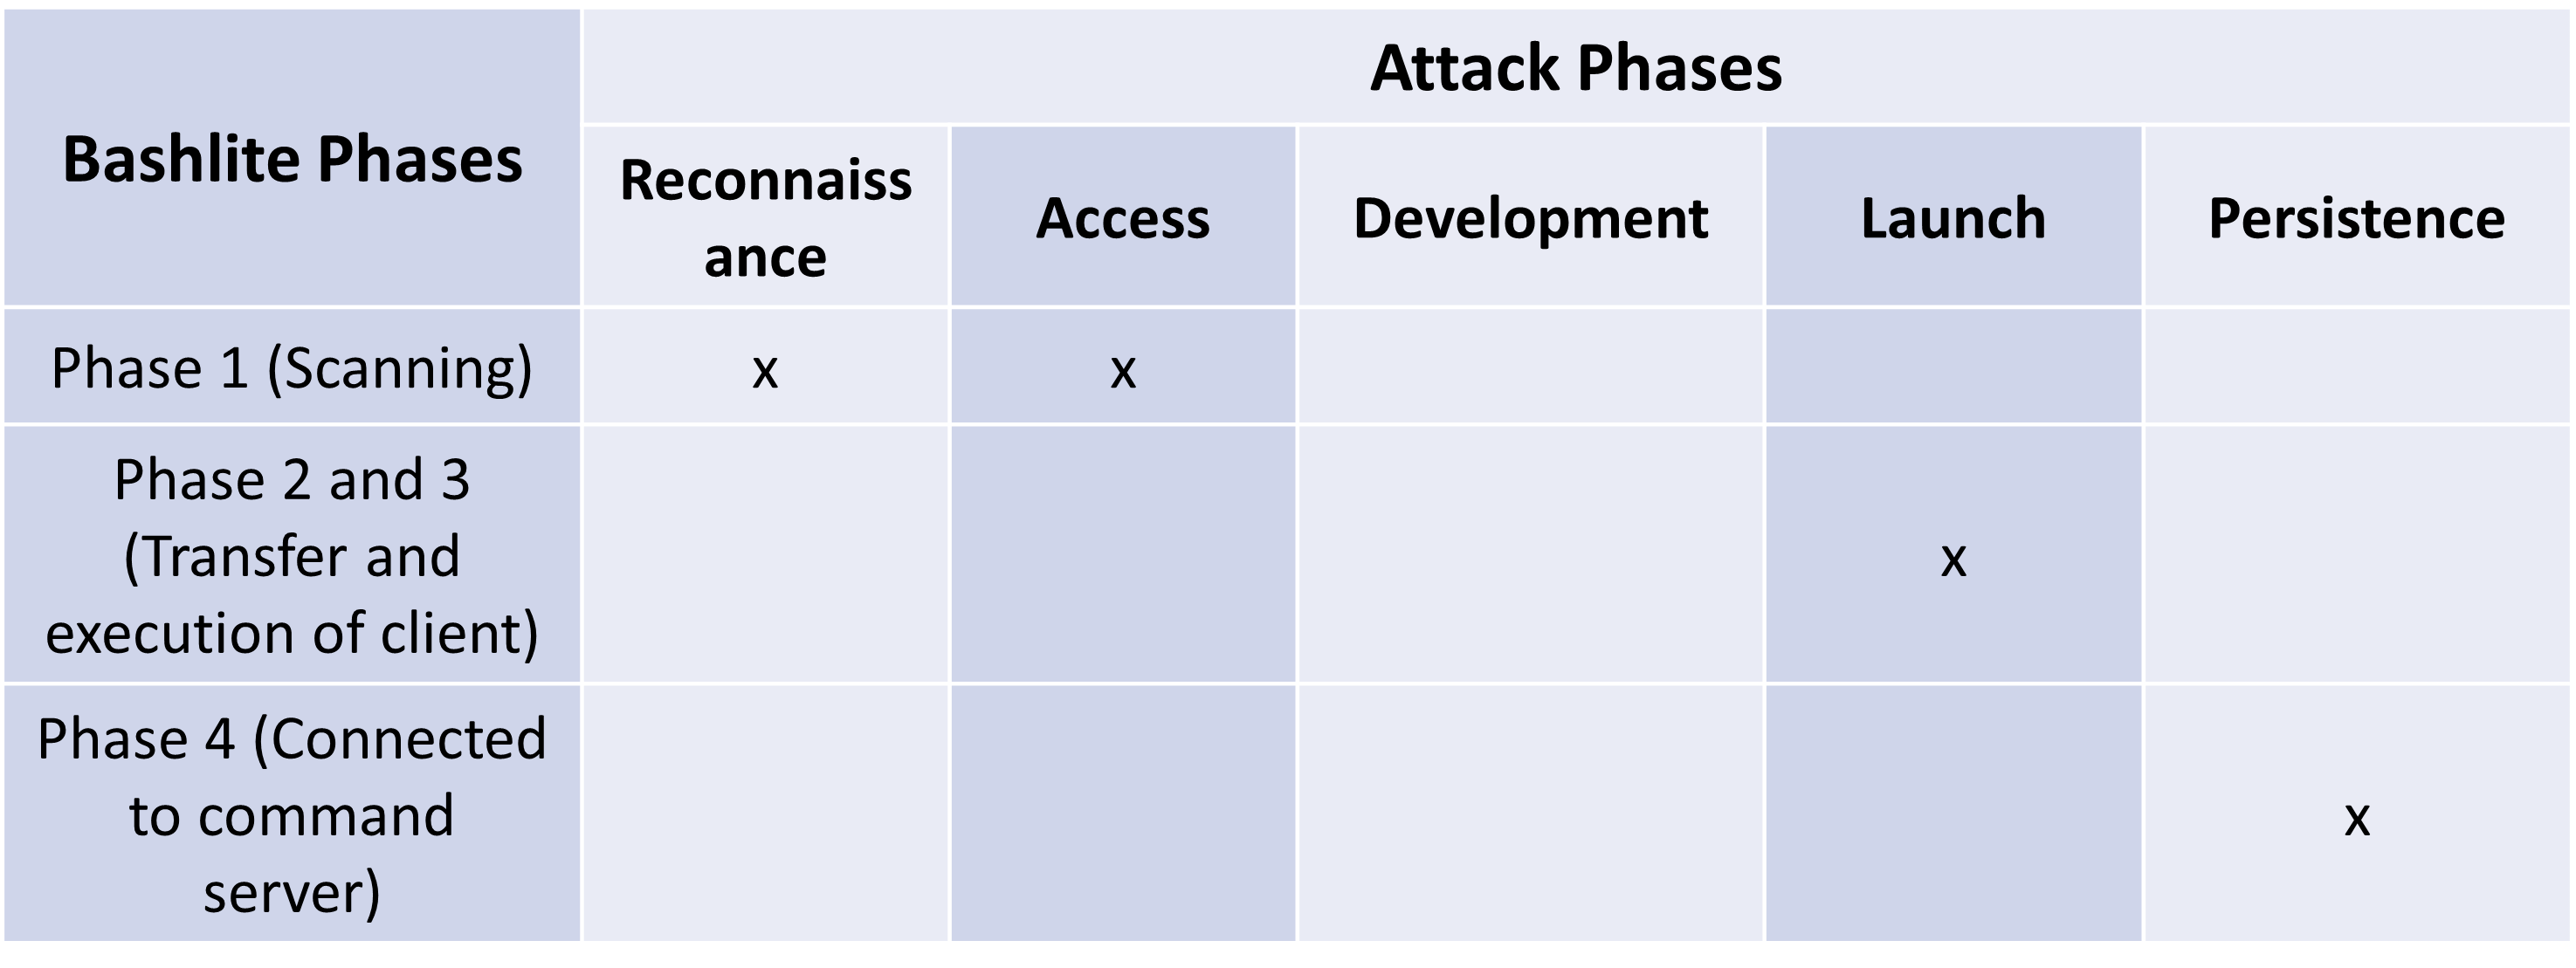
\includegraphics[scale=0.7]{assets/tableBashliteVSAttackPhases.png}
\centering
\caption{The Attack Phases of Bashlite and Their Mapping to the Corresponding Attack Phases.}
\label{graphic:tableBashliteVSAttackPhases}
\end{table}


Since Section \ref{analysisOfBashlite} showed in which phases of Bashlite it is possible to mitigate its infection, this can also be expressed in terms of the attack phases of~\cite{article:okhraviFindingFocus}. Hence, the MTD techniques applied defend against the Reconnaissance phase, the Access phase and the Launch phase.~\cite{article:okhraviFindingFocus} also indicated that Dynamic Network Domain techniques can hinder the Reconnaissance and Launch phases of an attack, but they did not indicate that Dynamic Network Domain techniques can also hinder the Access phase. I assume this is due to the difference in the type of attack (Bashlite vs. specific target).



\subsection{Issues of the Initial Prototype}
\label{section:IssuesOfInitialPrototype}
The first step towards the final implementation was to test whether the initial prototype would still run on the current machines. Unfortunately, this was not the case, as the \textit{ifconfig} command used to change the IP address in the initial prototype in Ubuntu was not suitable for changing the IP address in Raspberry OS. Another problem with the initial implementation was that each machine's IP address was changed. Assuming that a machine is infected and Bashlite starts scanning for other susceptible machines in the LAN, changing the IP address of the other machines would make no difference because Bashlite continues to scan for IP addresses randomly, meaning that another IP address would still be found. 
Furthermore, this thesis has not considered that the LAN setting could have other negative effects. Section \ref{section:futureResearch} briefly discusses this issue, but it was beyond the scope of this thesis to address it.   

%To make this an effective defense strategy for not yet infected devices, we would need to know which IP addresses are already scanned by Bashlite and Bashlite would not be allowed to start scanning again after it finished its scan. Unfortunately, I was not able to test this due to time constraints and my adaptions of Bashlite, but looking at the code of the client, this becomes obvious.  
%Besides of not knowing whether this would be technically feasible, the solution to change the telnet ports is much more convenient and secure. 


%As we have just seen, the IP change alone is not a suitable MTD techniques when dealing with Bashlite. In section \ref{analysisOfBashlite}, I discussed two possible MTD techniques that target the weaknesses of Bashlite and I chose to connect these two. The infected device will change its IP address, the other devices will move the telnet service away from port 23. Like that we can disconnect the infected IP from the command server and at the same time protect all other devices from getting infected. This combination has several advantages based on the type of botnet we look at. As we have seen in section \ref{subsection:P2PIoTBotnets}, P2P IoT botnets are extremely dangerous due to their robustness. My goal was that the solution ideally should protect against classic botnets as well as against P2P IoT botnets. In the following, I will first talk about my implementation and afterwards theoretically analyse how the implementation should work against these two different botnets. 

\subsection{Implementation Details}
This chapter presents and explains the implemented code. It separates the clients, \textit{Deployer Client} and \textit{Deployer Server} as well as possible, but the main goal was to explain the files in the order of the control flow. A recurring Python module in the code is the \textit{subprocess} module for running Bash commands in Python. Two different functions from this module were used, the \textit{subprocess.run()} and the \textit{subprocess.popen()}. A difference between the two is that the \textit{run()} function waits until the Bash command has finished, whereas the \textit{Popen()} executes the command in a child process~\cite{website:pythonSubprocess}. In practice, this means that \textit{subprocess.run()} will cause the Python code to pause its execution until the passed Bash command is complete, and \textit{subprocess.open()} will continue to execute the Python code without waiting for the Bash code to complete. Depending on the Bash command and its goal, it was clear which function was beneficial. 


\subsubsection{Device Sends Information} 
The starting script is \textit{sendToDeployerClient.py}. This script is quite simple and differs significantly from the initial prototype. First it connects to a listening socket created by the \textit{DeployerClient}. This is followed by a try and except block in which the scripts calls a function that starts Bashlite using the \textit{subprocess.Popen()} function. This ensures that Bashlite runs in the background and the Python script can continue. A modified version of Bashlite that immediately starts scanning for susceptible devices saved a lot of time, as there was no need to connect to the server as management and manually start the scanner over and over again. The \textit{sendToDeployerClient.py} script then sleeps for a certain number of seconds. This was to fake the time it took to detect Bashlite, as after this sleep the script sends a "malware found" message to the \textit{Deployer Client} listening socket.



\subsubsection{Deployer Cient Handling Client Information}
The listening socket of the \textit{Deployer Client} is created by the \textit{listenToDevices.py} script. Again, this is a fairly simple script that just listens for virus messages and calls the \textit{send()} function of the \textit{sendToDeployerServer.py} script. This listener supports multiple connections through multithreading. This was necessary because all devices in the LAN should be able to send information to the \textit{Deployer Client} at the same time. In the \textit{send()} function of \textit{sendToDeployerServer.py}, the script connects to the listening socket of the \textit{Deployer Server} and sends another virus message along with the IP address of the infected machine.




\subsubsection{Deployer Server Handling Deployer Client Information}
The \textit{listenToDeployerClient.py} script creates this listening socket and receives the virus message from the \textit{Deployer Client}. This message is then split to filter out the IP address, followed by a call to the main function of the \textit{sendToDevices.py} script with the IP address as an argument. This IP address argument indicates the IP address of the infected device. 

Before explaining the \textit{sendToDevices.py} script, this paragraph briefly explains the \textit{Config.json} file. This is where the user can add configuration values regarding the MTD techniques. The configuration file can be seen in Listing \ref{lst:Config}. There are several key-value pairs for each MTD technique (IP address and Telnet service port change). The rootIP, together with the startIPDevices and endIPDevices, determines the possible range of IP addresses that could be assigned to an infected device. So, in this listing example, the possible IP address of an infected device is in the range between 192.168.1.1 and 192.168.1.90 minus the IP addresses already in use. The server IP is generally used on multiple occasions throughout the code. As for the port change MTD technique, the "startOfPossible" and "endOfPossible" keys define the port range that could replace the Telnet service port on the susceptible devices. The "timeToChangeBack" key specifies the number of seconds that susceptible machines should wait before the Telnet service port is changed back to port 23. This information will eventually need to be sent to the client, but the aim was to have the entire configuration in one place.

\newcounter{temp}
\setcounter{temp}{\value{lstlisting}}
\setcounter{lstlisting}{0}
\renewcommand{\lstlistingname}{Listing}

\begin{lstlisting}[caption={The Configuration File in Which the MTD Values can be Specified.},label={lst:Config}]
{
"IP": {
  "rootIP": "192.168.1",
  "startIPDevices": "1",
  "endIPDevices": "90",
  "serverIP": "10"
  },
"port": {
  "startOfPossible": "3000",
  "endOfPossible": "4000",
  "timeToChangeBack": "300",
}}
\end{lstlisting}

\setcounter{lstlisting}{\value{temp}}
\renewcommand{\lstlistingname}{Algorithm}

The \textit{sendToDevices.py} is one of the two essential files. This file contains two functions. The first is a helper function called \textit{getIPInformation()}. This function takes a set of arguments specified in the Config.json file and returns an IP object containing all the relevant information regarding IP addresses. First, the function creates an array of all possible IP addresses within the range and the server IP address specified in the configuration. Then the function runs a \textit{nmap} scan on that IP range to see which IP addresses are already in use. The function filters the result of the \textit{nmap} with a regex expression, removes the occupied IP addresses from the array of all possible IP addresses, and creates an array in which it puts all occupied IP addresses except the server IP address and the infected IP address. This array is needed later and contains all the IP addresses that may need to move their Telnet service ports for the Telnet service. Finally, the object returned by the \textit{getIPInformation()} function is a dictionary with three key-value pairs containing the IP address of the infected device, the array of all possible/unoccupied IP addresses, and the array of all IP addresses that may need to change their Telnet service ports for the Telnet service.

The other function in the \textit{sendToDevices.py} is the \textit{letExecuteMTDMechanisms()}. This function triggers the start of the MTD techniques on the clients and provides them with the necessary information. It needs the information object returned by the \textit{getIPInformation()} function and other arguments from the configuration file. \textit{letExecuteMTDMechanisms()} starts by assigning the values of the information object to variables to keep the code as clean as possible. This is followed by two main blocks of code, the first dealing with the IP address change of the infected machine and the second dealing with the port change.


The code dealing with the IP address change starts with an if statement to check if an IP address was passed as a parameter in the function call. This allows the user to only change the port if he/she has a use for this, and it allowed to better test the code as it is possible to run the port change MTD technique alone. The if statement is followed by a try and except block to catch any errors. The try block connects to the infected device's listener, picks a random IP address from the array of all possible IP addresses, and sends a message of the form "IP:\textit{IPaddress}". But before this message is sent, a "-1" is sent to the listeners (clients) and the response is received. This was an improvised and slightly unclean fix, but since the client expects one more round of information from the \textit{MTD Deployer Server} in the port change code block than in the IP change code block, this allowed to leave the code as it was on the client side. After the IP message is sent, the port is closed. Again, several exceptions are caught to prevent unexpected code failures. The IP address change code block can be seen in Algorithm \ref{lst:Pseudocode sendToDevicesIP.py}.
\\

\begin{lstlisting}[                
    caption={The Code Block for Changing the IP Address on the Server Side From the \textit{letExecuteMTDMechanisms()} Function in Pseudocode. Everything Related to the Port Change has Been Ommited Here.},label={lst:Pseudocode sendToDevicesIP.py}]
def letExecuteMTDMechanisms(ipInformation,timeToChangeBack,maxTryOfNewPorts,startOfPossiblePorts,endOfPossiblePorts):
    // NOTE: omitted all the code for the port change
    
    SET allPossibleIPS to ipInformation["allPossibleIPs"]
    SET infectedIP to  ipInformation["infectedIP"]
    IF infectedIP is not None:
        TRY:
            CONNECT to client via socket
            SET newIP to random IP of allPossibleIPS
            SEND "-1" to client
            RECEIVE unimportant answer from client
            SEND "IP:newIP" to socket
            CLOSE connection to client
        CATCH ERROR:
            PRINT some kind of error message
    END IF
\end{lstlisting}

The code dealing with the port change starts with a for loop because, unlike the IP address change, the port needs to be changed on multiple devices. So the script iterates through all the IP addresses in the array of IP addresses that might need a port change. This is followed by another try and except block. Several things happen in this try block: a connection is made to the currently iterated IP address, an array is created containing all the ports defined as the port range in the configuration, and a random port is selected to be sent to the device. The script also sends the maximum number of attempts the client should make to migrate to another port. This is followed by two loops to continuously talk to the clients.

The inner while loop continuously sends a message ("port:\textit{Port}") with the randomly selected port to the client, which checks if the port is still available and sends a corresponding response. If the port is available, the script exits the inner loop and continues its execution. If the port is not available on the client, the port is removed from the array of available ports and a new port is randomly selected and sent again. In addition to these two options, the script also handles cases where the maximum number of ports to look up has been reached, or the ports on the client cannot be looked up at all. 

As soon as the code breaks out of the inner loop, the script does nothing, but waits for another message to be received. Here it checks three different cases: either the migration to the new port worked, an error was received, or the client asks for the time after which it should move the telnet service back to port 23. In the first two cases the script returns from the function, in the third case it sends the value of the \textit{timeToChangeBack} key from the configuration file. In the except block, the script catches a \textit{ConnectionRefusedError}, because if a device that should change the port of the Telnet service does not have the listener running, the code would otherwise throw an error and break. The code block for changing the port on the server side can be seen in Algorithm \ref{lst:Pseudocode sendToDevicesPort.py}.
\\

\begin{lstlisting}[caption={The Code Block for Changing the Port of the Telnet Service on the Server Side From the \textit{letExecuteMTDMechanisms()} Function in Pseudocode. Everything Related to the IP Address Change has Been Ommited Here.},label={lst:Pseudocode sendToDevicesPort.py}]
def executeMTDMechanisms(ipInformation,timeToChangeBack,maxTryOfNewPorts,startOfPossiblePorts,endOfPossiblePorts):
    // NOTE: omitted all the code for the IP change
    
    SET IPsToChangePort to ipInformation["IPsToChangePort"]
    FOR each IP in IPsToChangePort:
        TRY:
            CONNECT to IP of client via socket
            SET allPossiblePorts to range in config file
            SET newPort to random port of allPossiblePorts
            SEND maxTryOfNewPorts given in configuration file
            RECEIVE unimporTant answer from client
            SET success to False
            WHILE True:
                WHILE success is False:
                    SEND "PORT:newPort" to socket
                    RECEIVE answer from client:
                    IF answer is that port is free on client:
                        SET success to True
                    ELSE IF answer is that telnet port not retrievable:
                        PRINT some kind of error message
                        CLOSE connection to client 
                    ELSE IF answer is that max attempts are exceeded:
                        PRINT some kind of error message
                        CLOSE connection to client 
                    ELSE:
                        REMOVE newPort from allPossiblePorts
                        SET newPort to random port of allPossiblePorts
                    ENDIF
                END WHILE 
                SET answer to received data from client
                IF answer is that client finished:
                    PRINT success message
                    CLOSE connection to client
                ELSE IF answer is that error ocurred:
                    PRINT some kind of error message
                    CLOSE connection to client
                ELSE IF answer is that client needs num of seconds:
                    SEND seconds to move back from configuration
                ENDIF       
            END WHILE
        CATCH ERROR:
            PRINT some kind of error message
    END FOR
\end{lstlisting}

\subsubsection{Client Handling Deployer Server Information}
The \textit{listenToDeployerServer.py} is the most important script of the whole solution, as it actually executes the MTD techniques on the clients. This is the only script that needs to be run with \textit{sudo}, as some of the Bash commands included require this security privilege. 
The script has four small helper functions and one large helper function. The four small functions include one that writes to a log file called "output.txt", one that queries the current port of the Telnet service on the machine, one that checks if the Telnet service is listening on port 23, and one that kills a potential Telnet process. The logging functionality was crucial for debugging reasons. It helped to detect errors more quickly, and it is also essential in a real-world deployment of the MTD techniques. 
\\

The second little helper function was to query the current port of the Telnet service. This was needed because the change back to port 23 was not implemented from the start. This prevented the need to manually reset to port 23 after each run during the implementation process. More importantly, the Telnet service port query also catches possible errors that might occur in general. The \textit{getTelnetPort()} function first executes the Bash command shown in Algorithm \ref{lst:findTelnet}.

 \begin{lstlisting}[caption={The Bash Command Used to Query the Telnet Service Port.},label= {lst:findTelnet}]
ss -tlpHn | grep inetutils-inetd
\end{lstlisting}

The \textit{ss} command in Algorithm \ref{lst:findTelnet} can be used to examine sockets, similar to netstat~\cite{website:ss}. The options passed are: include tcp sockets, include listening sockets only, include processes, output information without the header, and try not to resolve service names~\cite{website:ss}. Additionally, the code filters with \textit{grep} for "inetutils-inetd", which was used as an identifier for the Telnet process. \textit{Inetd} is a program that listens on certain Internet sockets and decides which program should respond to the request~\cite{website:inet}. Using this as an identifier works perfectly on the VMs because Telnet is the only service on the VMs that uses \textit{inetutils-inetd}. As this may be different on other devices, it is possible that this Telnet port query may fail. To ensure that the script does not query the wrong port for the Telnet service and therefore misbehaves, the script also queries the Telnet service port from the \textit{/etc/services} file and compares the two. If they are identical, all is good, otherwise the script throws an \textit{AttributeError}. The reason for the \textit{AttributeError} is that it is needed anyway in case "ss -tlnpH | grep inetutils-inetd" returns nothing, which would lead to an \textit{AttributeError} caused by the regex the script uses to filter the port.

The third small but important helper function is the \textit{checkIfTelnetWorks()} function. This uses a socket to check if the Telnet service port allows a connection or not. This function is used to check if moving the Telnet service port was successful or not.

The fourth helper function is \textit{killTelnetProcess()}, which does exactly what it says, again using the \textit{subprocess.run()} function to execute the Bash command. The Bash command passed is a \textit{pkill} with an echo, which echoes either "True" or "False" depending on whether \textit{pkill} was successful or not, and logs accordingly.  


 The fifth and larger helper function is the most complex and is called \textit{changePort()}. It again starts with a command passed as an argument to the \textit{subprocess.run()} function. The command can be seen in Algorithm \ref{lst:replaceAndApply}.
 \\
 
 \begin{lstlisting}[caption={The Bash Commands to Replace the old Telnet Service Port With the new one and Apply the Change.},label={lst:replaceAndApply}]
sed -i 's/\<{0}\>/{1}/g' /etc/services
sudo systemctl restart inetutils-inet.service

\end{lstlisting}


The \{0\} and \{1\} in Algorithm \ref{lst:replaceAndApply} are placeholders which are inserted using Python's \textit{string.format()} function. The first line looks for the old Telnet service port number plus "/tcp" (e.g. 23/tcp) in \textit{/etc/services} and replaces it with the new port number plus "/tcp" (e.g. 2255/tcp). Initially, the mistake was made of not looking for the exact string, which led to other ports containing parts of the old port (e.g. 5523/tcp) being changed (e.g. to 552255/tcp). The solution was to surround the first placeholder with "<" and ">", which resulted in an exact search for the value to replace~\cite{website:sed}.

The second line of Algorithm \ref{lst:replaceAndApply} restarts the \textit{inetutils-inet} service, which applies the changes in the \textit{/etc/services} file without rebooting the system. The script then uses the \textit{grep} command to check if the new port can be found in \textit{/etc/services} and echoes accordingly. Depending on the echo, the script logs an error, returns from the function, or continues with the code. Next, the script uses the \textit{checkIfTelnetWorks()} function to see if the Telnet service is still listening on port 23. If it is, the script writes an error to the log file and sends an error message back to the \textit{Deployer Server}. Otherwise, the code logs that the Telnet service is no longer listening on port 23 and sends a "done" to the \textit{Deployer Server}. Additionally, the script triggers the Telnet service to change back to port 23 after a certain number of seconds. This number is also specified in the \textit{Deployer Server} configuration file. 
To initiate this change back, the script uses the \textit{subprocess.Popen()} function instead of the \textit{subprocess.run()} function, as the Python script should continue to run. The command passed as an argument to \textit{subprocess.Popen()} can be seen in Algorithm \ref{lst:backToPort23}.
\\

 \begin{lstlisting}[caption={The Bash Commands to Change Back to the Telnet Service Port 23 Afer a Given Number of Seconds},label={lst:backToPort23}]
printf "$(date +%F\ %H-%M-%S) SHELL: Sleeping for {0} seconds\n" >> output.txt
sleep {0}
sed -i 's/\<{1}\>/23\/tcp/g' /etc/services
sudo systemctl restart inetutils-inetd.service
sleep 7
sudo lsof -i:23 && found="true"
if [ "$found" = "true" ]
then
    printf "$(date +%F\ %H-%M-%S) SHELL: Went from port {2} back to port 23\n\n\n" >> output.txt
else
    printf "$(date +%F\ %H-%M-%S) SHELL: ERROR: The change back to port 23 failed somehow\n\n\n." >> output.txt
fi       
\end{lstlisting}

The first two lines of Algorithm \ref{lst:backToPort23} write a log to the same file where the Python code is logged. Then the script sleeps for the specified number of seconds. Again, these numbers are inserted using Python's \textit{string.format()} function. Lines 4 and 5 are almost identical to the \textit{changePort()} function, except that the target port is now port 23 again. After modifying the \textit{/etc/services} file, the \textit{inetutils-inted.service} is restarted to take effect without rebooting the machine. The script then pauses for 7 seconds to allow the changes to the port to take full effect before continuing. On line 7, the script runs a \textit{lsof} command to check if port 23 is listening again. This is the Bash replacement for the \textit{checkIfTelnetWorks()} function in Python. Ideally the script would check directly with Telnet if the connection is possible, but it was not possible to make this work with the \textit{subprocess} module. If port 23 is listening, the script logs a success message to the log file (on lines 8 and 9), otherwise it logs an error to the log file (on lines 10 and 11). 


The main function of the \textit{listenToDeployerServer.py} script is \textit{listenToDeployer()}. First the listening socket is created, followed by the first while loop. In this loop, the script receives the maximum number of attempts to look for a free Telnet port sent by the \textit{Deployer Server}, which queries the configuration file for the maximum number of attempts. The script then sends a response that the maximum attempts have been received, which also ensures that the \textit{Deployer Server} does not continue with its code as it is forced to wait for a response. A second loop follows in which the script receives another message from the \textit{Deployer Server} that is either "IP:\textit{IPaddress}" or "port:\textit{Port}". This message is split into two variables called "movingParameter" and "movingParameterValue". The script then checks whether the moving parameter is "IP" or " port".

In the IP case, the script closes the listening socket properly, as it would have been closed anyway after the IP change, and all the necessary information has been received. It then kills the Bashlite process. Although the IP change disconnects the Bashlite client from the command server, rendering it harmless, the Bashlite client continues to run on the infected machine, which was tedious for testing. Therefore, the Bashlite client was killed. The IP address of the device is then changed using the command shown in Algorithm \ref{lst:replaceApplyIP}.
\\

\begin{lstlisting}[caption={The Bash Commands to Change the IP Address.},label={lst:replaceApplyIP}]
sed -i 's/\<{0}\>/{1}/g' /etc/dhcpcd.conf
ifconfig eth0 down && sudo ifconfig eth0 up
                
\end{lstlisting}


The first line of Algorithm \ref{lst:replaceApplyIP} replaces the old IP address with the new one in the \textit{etc/dhcpcd.conf} file. The script again inserts the values in Python with the \textit{string.format()} function, therefore the \{0\} and \{1\} in the Bash code. The second line shuts down the Ethernet adapter and restarts it immediately. The Raspberry OS needs to do this to migrate to the new IP address, otherwise the changes would not take effect until the system is rebooted, which is not applicable. After the IP address is changed, the script sleeps for 7 seconds because the Ethernet adapter needs about 5 seconds to reboot. After this time, the script uses the \textit{socket.gethostbyname()} function to get the current IP address of the device, checks whether the IP address change worked or not, and logs a corresponding message. The Python code block for changing the IP address on the clients can be seen in Algorithm \ref{lst:Pseudocode listenToDeployerServerIP.py}
\\

\begin{lstlisting}[caption={The Code Block for Changing the IP Address of a Client From the \textit{listenToDeployer()} Function in Pseudocode. Everything Related to the Port Change of the Telnet Service has Been Ommited Here.},label={lst:Pseudocode listenToDeployerServerIP.py}]
def listenToDeployer(HOST, PORT):
    CREATE listening socket
    WHILE True:
        RECEIVE max attempts for trying to find port (-1 here)
        SEND unimportant answer
        WHILE True:
            RECEIVE command from server
            SPLIT command to movingParameter and movingParameterValue
            IF movingparamter is "IP":
                CLOSE connection to client
                KILL telnet process
                CHECK if telnet process was killed
                CHANGE the IP address
                SLEEP for 7 seconds
                CHECK if the IP change worked
            // NOTE: omitted all the code for the port change
            ELSE
                CLOSE socket
                RETURN
            ENDIF
            
\end{lstlisting}

If the moving parameter is the port, then another machine in the network is infected and the current machine should move its Telnet service port. There is an additional condition in the port case if statement. This condition is whether a count variable is below the maximum number of port change attempts.

The port change code block is more complex than the IP change block above. In a first step, the script checks the \textit{/etc/services} file to see if the random port sent by the \textit{Deployer Server} is free on this device. If the port is found in the services file, the script sends a "taken" message to the \textit{Deployer Server}, which then sends a new random port as described above. If this port is free on the device, the script will query the current Telnet port using the \textit{getTelnetPort()} function described above. The script also calls the \textit{killTelnetProcess()} function. This is necessary because, as mentioned above, if the Bashlite server has already started a connection to this susceptible machine, changing the port of the Telnet service would have no effect, and the Bashlite client would normally start on the susceptible machine. 

Note that the \textit{killTelnetProcess()} function only affects existing connections, not an open Telnet service in general. Nevertheless, the function is called anyway, as there is no downside to calling it. The script then uses the \textit{checkIfTelnetWorks()} function described above to check if the current Telnet service is running on the machine on port 23 or not. If not, the script returns from the \textit{listenToDeployer()} function and logs accordingly, as no measurements are required. Otherwise, the port change is initiated by another function called \textit{changePort()}, which is described in more detail above. This function changes the port of the Telnet service from 23 to another random port sent by the \textit{Deployer Server}, checks if this port change worked, and also changes the Telnet service back to port 23 after a given number of seconds. After this function finished, the socket is closed and the script returns from the \textit{listenToDeployer()} function. The code block for changing the port of the Telnet service on the clients can be seen in Algorithm \ref{lst:Pseudocode listenToDeployerServerPort.py}.
\\





\begin{lstlisting}[caption={The Code Block for Changing the Port of the Telnet Service of a Client From the \textit{listenToDeployer()} Function in Pseudocode. Everything Related to the IP Address Change has Been Ommited Here.},label={lst:Pseudocode listenToDeployerServerPort.py}]
def listenToDeployer(HOST, PORT ):
    CREATE listening socket
    WHILE True:
        SET count to 0
        RECEIVE max attempt for trying to find port
        SEND unimportant answer
        WHILE True:
            RECEIVE command from server
            SPLIT command to movingParameter and movingParameterValue
            IF movingparamter is "IP":
                // NOTE: omitted the code for the IP address change
            ELSE IF movingParameter is port and count <= max attempt:
                INCREMENT count
                CHECK if movingParameterValue (port) is used
                IF port is used:
                    SEND that port is already used
                    CONTINUE with WHILE loop
                ELSE
                    CALL function to get telnet port
                    IF not possible:
                        SEND error
                        CLOSE socket
                        RETURN
                    END IF
                    SEND that port is unused
                    CALL function to kill existing telnet processes
                    CALL function to check if telnet listens on port 23
                    SEND message to get the time to change back
                    RECEIVE time to change back
                    CALL function to change port
                    CLOSE socket
                    RETURN
            ELSE
                SEND max attempt are exceeded
                CLOSE socket
                RETURN
            ENDIF
            
\end{lstlisting}





% bis do ane de text korrigiert und mit writefull drüber








\begin{comment}
\subsection{Things that I could have done differently}
rite bashlite such that it checks for open ports in the lan 

%\subsection{Potential Problems} \label{section:potentialProblems}
When we consider the LAN setting, Bashlite could also theoretically scan for IP addresses in the network as well as all possible ports for this IP devices. I did not create such a Bashlite version, but I   
theoretisch wärs chillimarili zum im bashlite client checke zum d'ip vom host gwechslet het und denn eifach neu zum command server verbinde


\todo{remove the deployer client, it is basically useless and just an additional poit of faiulre and a  similartiy to jordan}
\end{comment}
%\input{.tex}
%\input{.tex}
\chapter{Evaluation}
This chapter presents the evaluation of the implemented Moving Target Defense (MTD) framework with its techniques based on different criteria. First, the methodology of the evaluation is explained, followed by the missing prerequisites for the evaluation to work. The chapter then presents the evaluation process and its results. These results are discussed in Chapter \ref{chapter:discussion}.


\section{Evaluation Methodology} \label{section:evaluationMethodology}
The evaluation of the solution was quite complex because the whole setup had so many parts/scripts distributed across three different VMs. Ultimately, three different metrics were to be evaluated. The first and main evaluation metric is the total number of seconds that the two machines in the network are infected. This is reasonable as the goal of this thesis is to mitigate/prevent the infection of IoT devices and to show that a collaborative approach yields better results than a non-collaborative one. Thus, the fewer seconds the malware is running on the devices, the better. The other two metrics are defender metrics mentioned by~\cite{article:surveyMTD}, who investigated MTD research trends. Both metrics fall into the system performance category. 

The first system performance metric is the amount of time that incoming and outgoing communication to and from the device is interrupted. This can be further divided into the interruption caused by the IP address change and the interruption caused by the Telnet service port change. For the IP address change, only the outgoing connection was tested. The reason for this is that the incoming connection would only work if there was a mechanism to keep track of which machine has which IP address, similar to the one suggested by~\cite{NavasDefenseFramework}. However, outgoing connections are more critical, as IoT devices often need to pass on collected data. Regarding the Telnet service port change, incoming and outgoing connections to and from the Telnet port were evaluated. The other system performance metric is the CPU/RAM usage of the deployed MTD techniques, which is essential due to the hardware limitations of IoT devices.


Other potentially important metrics~\cite{article:surveyMTD} such as Quality of Service (QoS) to users or strategy switching costs were not included. This exclusion is due to the fact that these metrics were either out of scope or not feasible (e.g. power consumption). The three measured metrics were therefore:
\begin{enumerate}
    \item Total number of seconds that the machines are infected 
    \item Interruption of network availability of the machines
    \item CPU/RAM usage of the framework and the executing MTD techniques

\end{enumerate}

These metrics were measured in three different environments/systems for comparison. All environments used the VM structure already described, but differed in the solution applied and their deployment strategy (i.e. proactive vs. reactive deployment of MTD techniques). Environment 1 used a reactive, modified solution that did not include a cooperative component. This was done by only enabling the IP address change of infected machines. This approach already exists~\cite{article:vonderAssen}, but the implementation code of the approaches are independent. This environment allowed the collection of data from a solution that uses a non-cooperative and reactive defence approach, and served as a baseline for this evaluation. 

In contrast, Environment 2 used the IP address and the port change to reactively mitigate/prevent Bashlite. This environment allowed to collect data from a solution that uses a cooperative and reactive approach. Environment 3 used the cooperative approach (IP address change and Telnet service port change), but executed this proactively rather than reactively. This provided an interesting insight into the trade-offs/differences between the proactive and reactive approaches. While the reactive approaches were executed 10 seconds after Bashlite was executed, the proactive MTD techniques were executed every 60 seconds, regardless of whether Bashlite was active or not. The 60 seconds were initially chosen randomly, but proved to be a reasonable value given the results. Furthermore, the goal was to show the typical differences between the reactive and proactive approaches, rather than to determine an optimal time to move, as this would be influenced by many more factors of the system. Table \ref{graphic:tableEvaluationEnvironment} summarises the three environments.

The data was collected over 30 runs (entire infection/mitigation process) in each environment and is presented in Section \ref{section:results}. The first five of these 30 runs were removed from the data as they were used to warm up the entire system. Section 
\ref{section:gatheringData} describes the data collection in more detail. 


\begin{table}[tph]
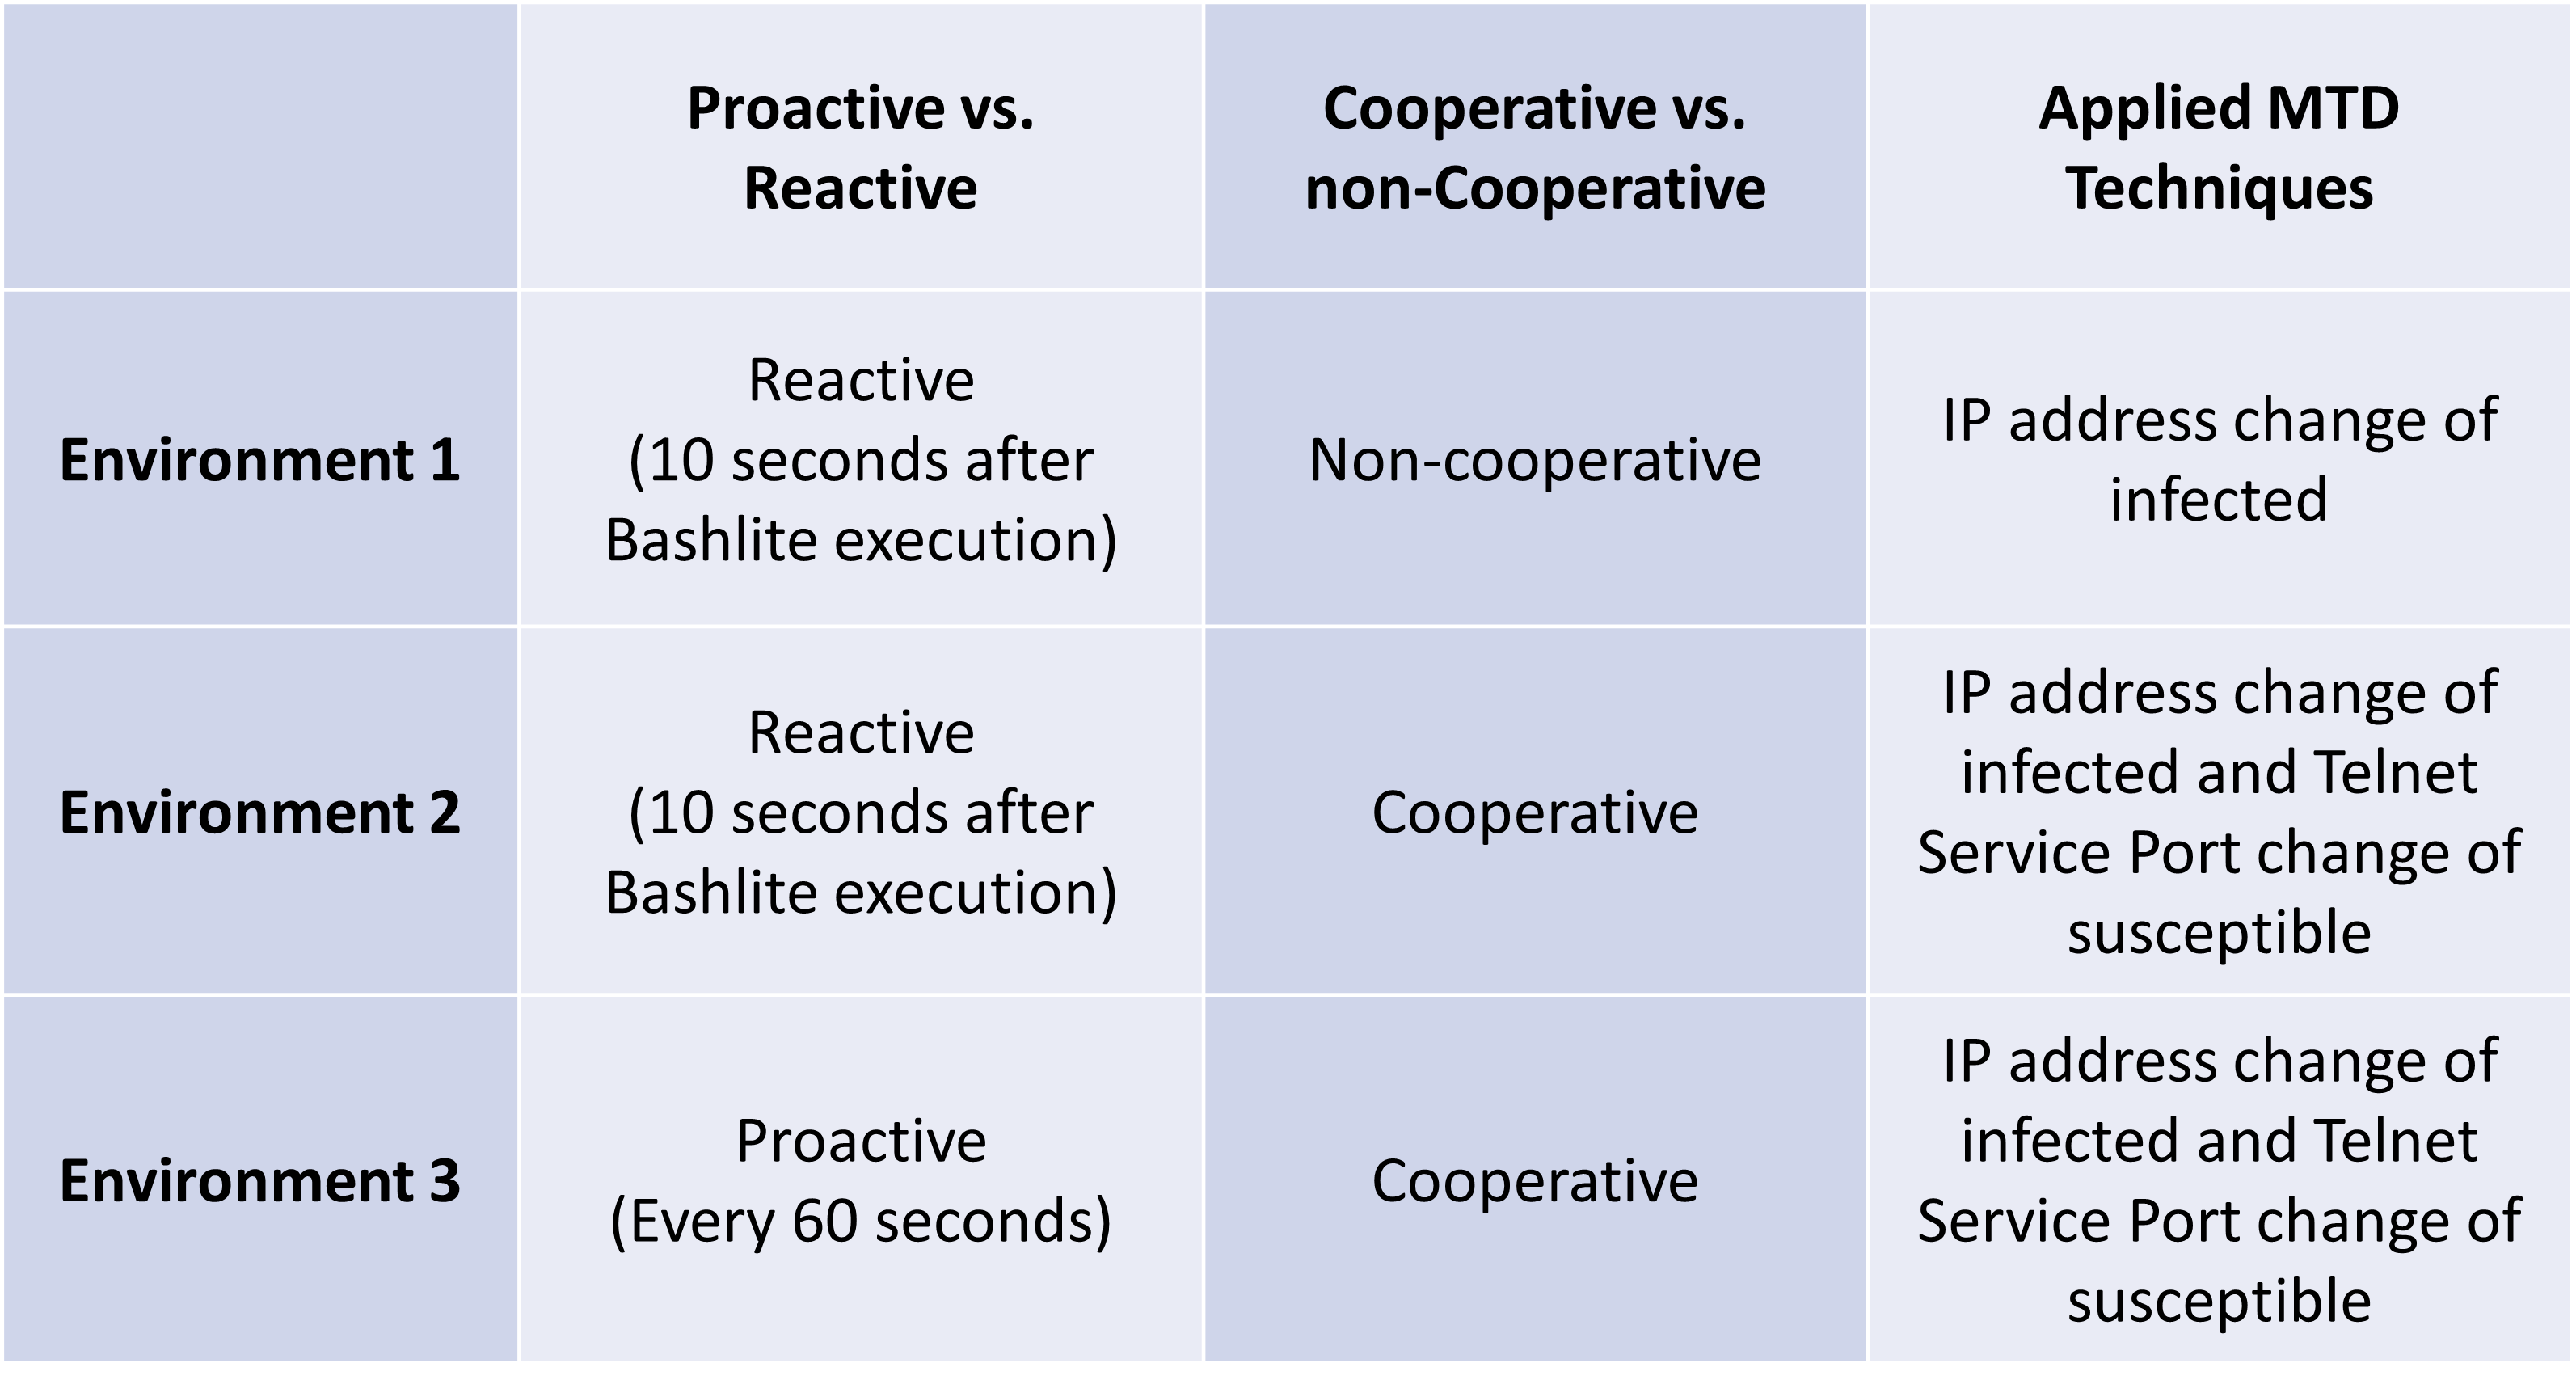
\includegraphics[scale=0.65]{assets/tableEvaluationEnvironment.png}
\centering
\caption{A Table Showing the Characteristics of Three Different Environments in Which the Previously Defined Metrics are Measured.}
    \label{graphic:tableEvaluationEnvironment}
\end{table}




\section{Prerequisites for the Evaluation}
Even though the implemented MTD mechanism worked, its code had to be adapted on several occasions. This involved three main tasks:
\begin{enumerate}
\item Writing scripts to measure and log the metrics, such as how long Bashlite has been running on the machine. 
\item Automating the code as much as possible. To get a reasonable amount of data, the infection/mitigation process had to be run multiple times, which was not feasible by hand. The idea was to be able to run the whole process once and then repeat it \textit{n} times.
\item Modifying the current scripts to fit the different environments. This included, for example, the adaptation that no Telnet service port change was triggered in Environment 1.
\end{enumerate}

The following subsections briefly describe how these tasks were accomplished. However, first an important aside regarding the Bashlite client. There was the problem that it was not possible to check whether a Bashlite client was still connected to the Bashlite server or not. To solve this, the killing of the Bashlite client in the IP address change technique remained in the code. This was justified by extensive testing and the existing literature~\cite{article:vonderAssen} regarding the interruption of the connection between the server and the client, and because the evaluation would simply not have been possible otherwise. Moreover, Bashlite is killed as soon as the client loses connection to the server, so there is only a negligible difference in time. This allowed the simplification that if a Bashlite client was running on the system, it was also connected to the server and vice versa. 


\subsection{Data Collection} \label{section:gatheringData}
Having solved this problem, a mixture of Bash and Python scripts were written to log the data into some .csv files, which were later analysed and plotted using Python. The reason for using both types of script was that sometimes one or the other was more suitable. This resulted in several files. 

The \textit{stopTimeOfClient.sh} script checks every 0.05 seconds whether the client process is running on the machine. If it is, the script stores the time of the start of the client, waits for it to finish and writes all the information to a \textit{bashliteAnalysis.csv} file. This script is continuous and also indicates which Bashlite run the system is on.

The \textit{CPURamAnalysis.py} script uses \textit{psutil} to monitor the CPU and RAM usage of the system and writes this to a CPURamAnalysis.csv file. The original idea was to specifically measure the CPU and RAM usage of the script that executes the MTD techniques on each machine. However, as the CPU usage of the script was almost always 0\% (measured with Bash/top and Python/psutil to exclude errors), a graph showing this would not give much insight. Thus, only the RAM usage was measured with \textit{psutil} since this was giving correct and measurable results. The CPU usage of the infected and susceptible machines was measured once with the MTD mechanism deployed and techniques executing, and once without the MTD mechanism deployed. This allowed to compare the case with MTD to the case without MTD on the respective machine. Both measurements were run for 15 infection/mitigation runs, equivalent to 30 minutes.  

%This gives a indication about how hardware intensive the actual execution of the MTD techniques is, since for example the IP change is only executed when Bashlite is active. Thus, it was possible to compare the system without executing MTD techniques against the system where the MTD are executed and Bashlite is active. The maximum CPU used can therefore not be higher than the difference between these two cases. Another reason why this approach made sense is that the defense mechanism on the clients are intended to run permanently, because they need to listen to potential attacks. 

The \textit{sendPacketsToServer.sh} script monitors outgoing packet losses. This is achieved by sending simple one-packet pings to the server machine every 0.5 seconds. The script also keeps track of the current Bashlite run. This gives interesting insights for the different environments. In Environment 1 and 2, outgoing packet losses should only occur once per Bashlite run, as the MTD techniques are executed reactively. In Environment 3, the MTD techniques are executed proactively, and therefore multiple packet losses are possible during a Bashlite run. All this information is written to a \textit{packetLoss.csv} file.

The \textit{telnetToLocal.py} and \textit{telnetToLocalOnlyIP.sh} scripts were written to track the interruption of the incoming Telnet service from the susceptible machine. The former was created first and uses \textit{sockets} (or \textit{telnetlib}) to check whether port 23 of the executing machine is listening or not. This produced reliable results, but there was an issue in the non-cooperative environment due to the two possible IP addresses the susceptible machine could have. Sockets in general were too slow to either get the host IP address or try to connect to both possible IP addresses, so a shell script that uses \textit{netcat} to check whether port 23 of both possible IP addresses are listening was more suitable. All this information is logged to a file called \textit{telnetToLocal.csv} or \textit{telnetToLocalOnlyIP.csv} depending on which script was used.

The \textit{telnetToServer.py} file is the last script and monitors whether outgoing telnet connections are possible or not. It does this using the \textit{telnetlib} module as in this case, it was essential to use Telnet as the communication protocol for the outgoing connection. 

%\todo{es wär mega guet zum eh grafik mache woni d'vms han, iwie usgehendi und ihkommendi pfiil wo ahgebed wele weles file was catcht }



\subsection{Automation}
Regarding automation, the implementation code already fulfilled most of the requirements. Only four issues remained. The first was that the script \textit{sendToDeployerClient.py} from VM1 needed some adaptations to separate the start of Bashlite from the start of the defence technique (notifying the \textit{Deployer Client}). One reason for this was the parent/child relationship between Bashlite and the Python script, which made it impossible to kill Bashlite (the child) while the Python script (the parent) was still running. Creating another Bash script called \textit{startBashAndSendToDepClient.sh} solved this problem. This file contains a while loop with each iteration being an entire infection/mitigation process. First, the while loop starts the Bashlite client and then sleeps for 10 seconds, mimicking the time it takes to detect Bashlite. After this time it starts the \textit{sendToDeployerClient.py} in the background and then sleeps again for 110 seconds. This time period could also be shorter, but it ensured that the previous infection process is completed with all the corresponding MTD techniques. 

The second problem was that the \textit{sendToDeployerClient.py} script had to be triggered somehow on VM2 as well. It was not possible to use the same script as for VM1 (\textit{startBashAndSendToDepClient.sh}), since this started Bashlite manually on VM1 and VM2 needed to detect it somehow. The solution was a Bash script that runs continuously and checks if Bashlite is running. If Bashlite is running for more than 10 seconds, the script executes \textit{sendToDeployerClient.py} which then initialises the MTD mechanism. This functionality was implemented with a shell script called \textit{checkForBashliteAndStartMTD.sh}. 

The third encountered issue was that the Bashlite server would only allow one infection, after which a restart of the server was required. This was added at the beginning of the thesis to improve stability, as the Bashlite client was constantly sending the same report about the susceptible machine, causing the Bashlite server to crash. Since it was not an option to always restart the server manually, the Bashlite client was adapted to send the report only once, and thus the restriction on the Bashlite server could be removed. 

The fourth issue was that about 15 scripts per environment would have had to be started to get everything running. To avoid this, a Bash script (\textit{runAll.sh}) was written containing all the startup instructions for each machine and environment. This resulted in three different startup scripts on three different machines, which was acceptable. Additionally, the counterparts for terminating all scripts started by \textit{runAll.sh} were created. This allowed to quickly start all the scripts, let them collect data and then terminate them effortlessly.

\subsection{Creating Evaluation Environments}
Finally, the different environments/systems had to be created. The first environment was the non-cooperative one, which only involved changing the IP addresses of the infected machines. 
The only required server-side adaptation was to instruct the \textit{Deployer Server} not to initiate any Telnet service port changes. This was done by replacing the array containing all the IP addresses that were potentially going to receive a port change with an empty array. 

On the client side, there was the problem that the Bashlite client was only scanning one IP address for a susceptible machine, so as soon as the IP address change was executed on VM2, the Bashlite client on VM1 would no longer find VM2 in the next Bashlite run. To solve this, two hardcoded IP addresses replaced the IP address variable received from the \textit{Deployer Server}. Thus, VM2 simply switches between these two IP addresses instead of migrating to the one sent by the \textit{Deployer Server}. This allowed adapting the Bashlite scanner of the client of VM1 to try only two different IP addresses, which worked perfectly. Note that this was only needed for the evaluation as the Bashlite implementation is limited. If it were not for the evaluation, or if Bashlite was scanning in a more sophisticated way, this adaptation would not be required at all. Besides, this did not make any difference to the data collected.

The second environment was the original idea, which was Bashlite together with a cooperative MTD approach. Since this usecase was the goal from the start, nothing had to be changed. The third environment involved Bashlite with the proactive MTD execution. To create this environment, the only required adaptation was to split the \textit{startBashAndSendToDepClient.sh} script into two subscripts. The first script starts the MTD mechanism every 60 seconds, the second script starts Bashlite randomly at an interval between 60 and 90 seconds. These two scripts are then executed by the \textit{runAll.sh} script. 




\section{Results} \label{section:results}
This section presents the results of the evaluation. It is divided into the three metrics mentioned in Section \ref{section:evaluationMethodology}, namely the duration of infection activity in the network, the interruption of availability, and the CPU/RAM usage. 

\subsection{Duration of Infection Activity in the Network}
The duration of infection activity was the most important metric as it defined whether the defence mechanism was working or not. Figure \ref{graphic:tableEvaluationEnvironment} shows the results for Environment 1, which was the non-cooperative and reactive solution. On the x-axis is the current run (infection/mitigation process). The blue bar of the stacked bars shows the number of seconds that VM1 was infected with Bashlite, meaning that Bashlite lasted approximately 29 seconds on VM1 in each run. The orange bar shows the number of seconds that VM2 was infected, which was also approximately 29 seconds per run. This gave an average of 57.6 seconds of total infection activity on the two VMs per run. It is evident that in this non-cooperative approach, the spreading to the susceptible machine could not be prevented at all. Bashlite was still mitigated, but each machine had to clean itself after the infection had occurred. 

\begin{figure}[tph]
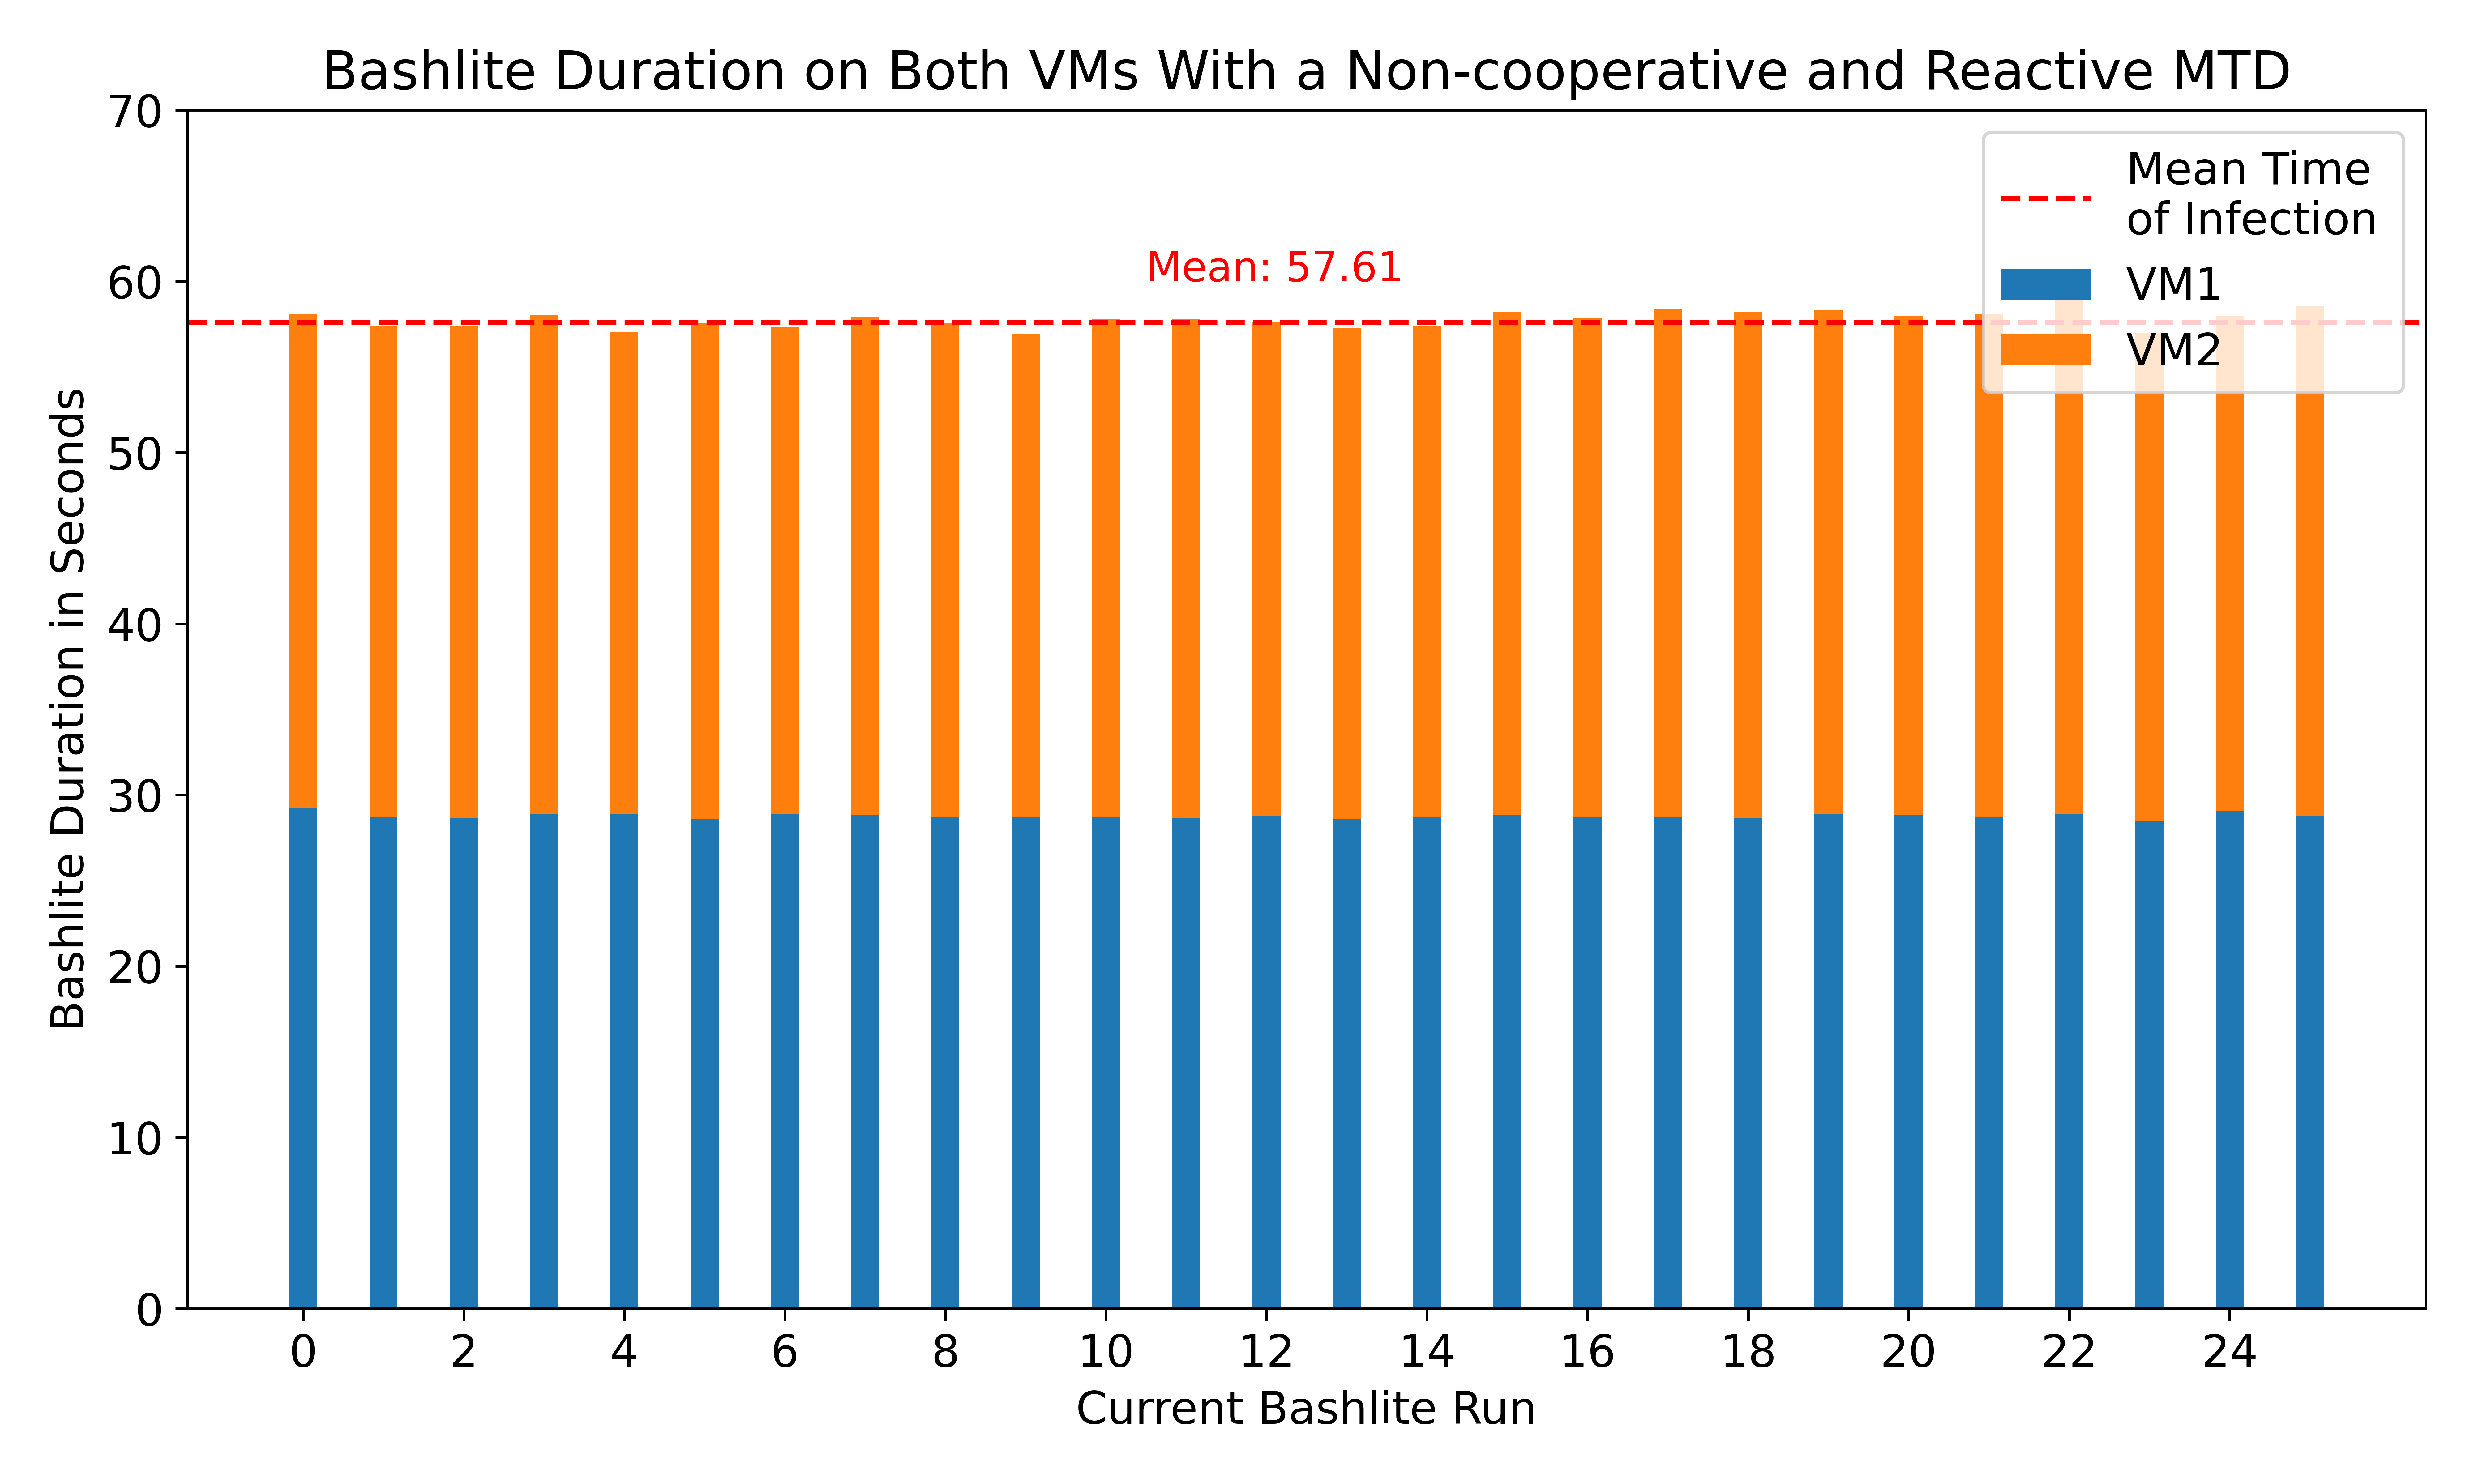
\includegraphics[scale=0.6]{assets/bashliteDurationUncoopAndReactive.png}
\centering
\caption{The Duration of Infection Activity on Both Virtual Machines in the Non-cooperative and Reactive Environment.}
\label{graphic:tableEvaluationEnvironment}
\end{figure}

Figure \ref{graphic:bashliteDurationCoopAndReactive} shows Environment 2, which was the cooperative and reactive environment. Again, the blue bars represent the number of seconds that VM1 was infected, the orange bars would represent the time that VM2 would have been infected if this had occurred. It is evident that in the cooperative and reactive environment the spreading to VM2 was prevented in every run. This resulted in an average of about 28.8 seconds of total infection activity on the two VMs, which is approximately half of the time of the uncooperative and reactive environment. 






\begin{figure}[tph]
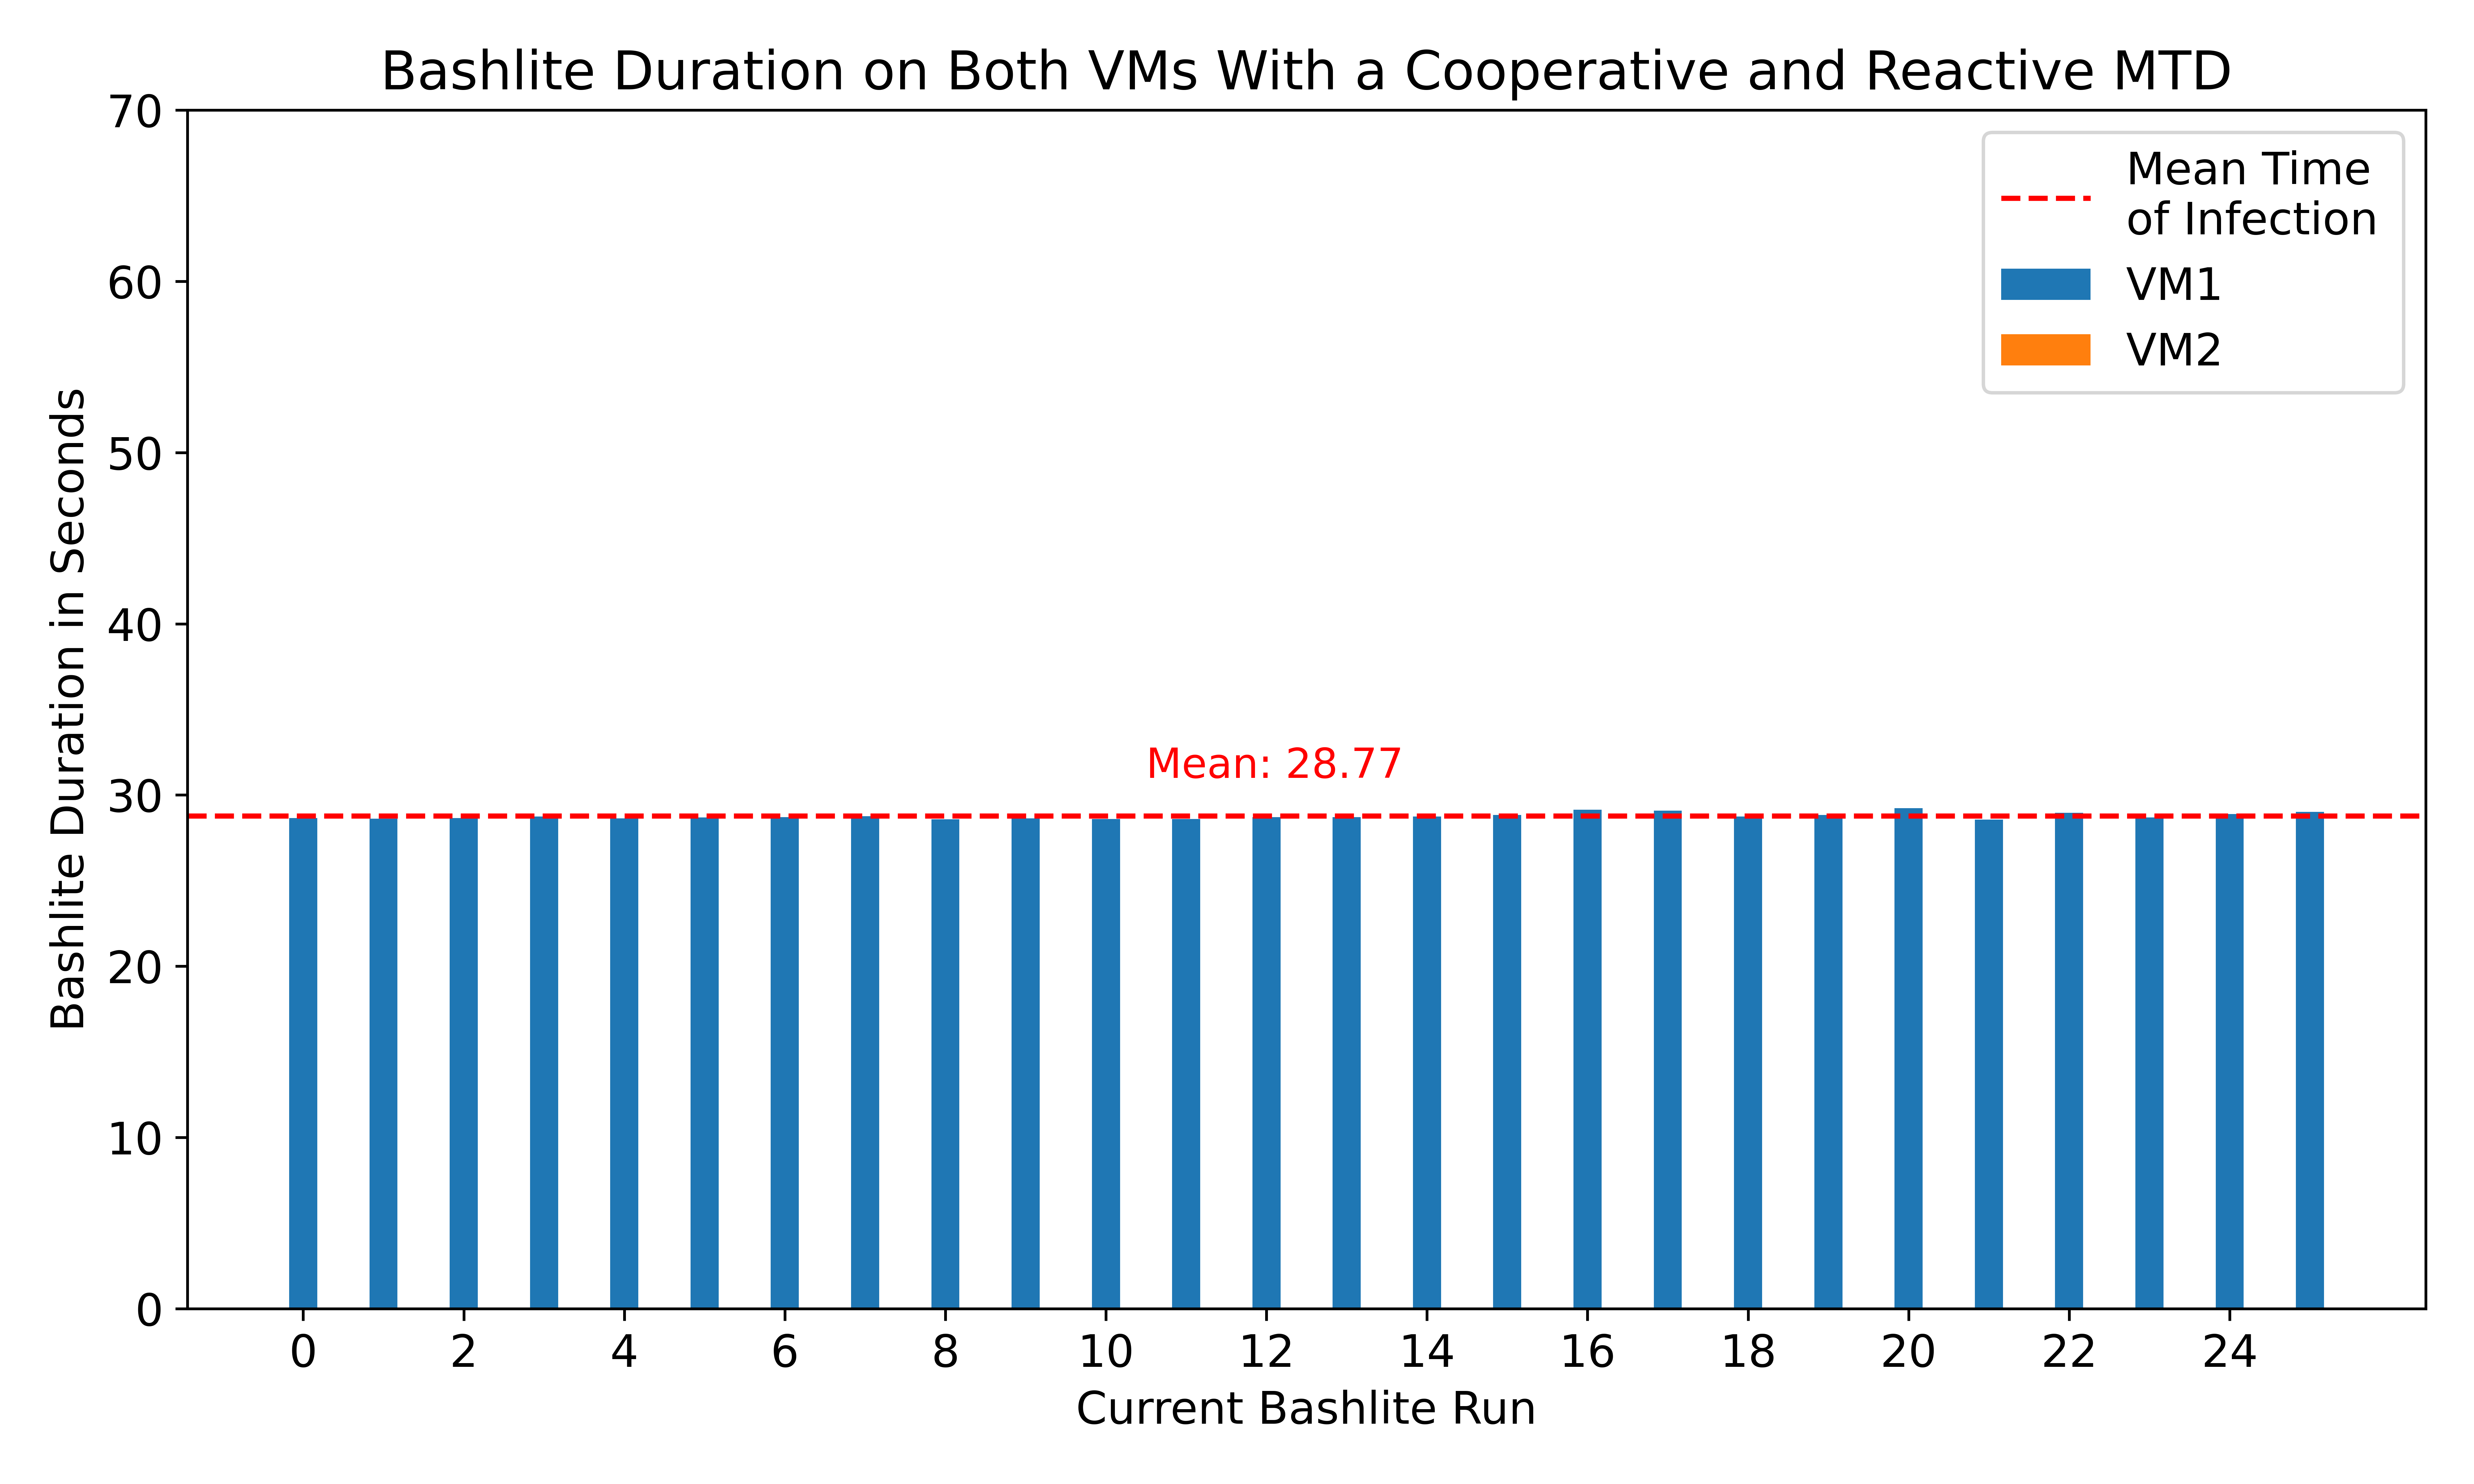
\includegraphics[scale=0.6]{assets/bashliteDurationCoopAndReactive.png}
\centering
\caption{The Duration of Infection Activity on Both Virtual Machines in the Cooperative and Reactive Environment.}
\label{graphic:bashliteDurationCoopAndReactive}
\end{figure}


Figure \ref{graphic:bashliteDurationCoopAndProactive} shows Environment 3, which was the cooperative but proactive environment. Unlike the previous two environments, the Bashlite duration was different for each run. The mean duration was slightly higher than the mean duration of the cooperative and reactive environment, but much lower than that of the non-cooperative and reactive environment.   





\begin{figure}[tph]
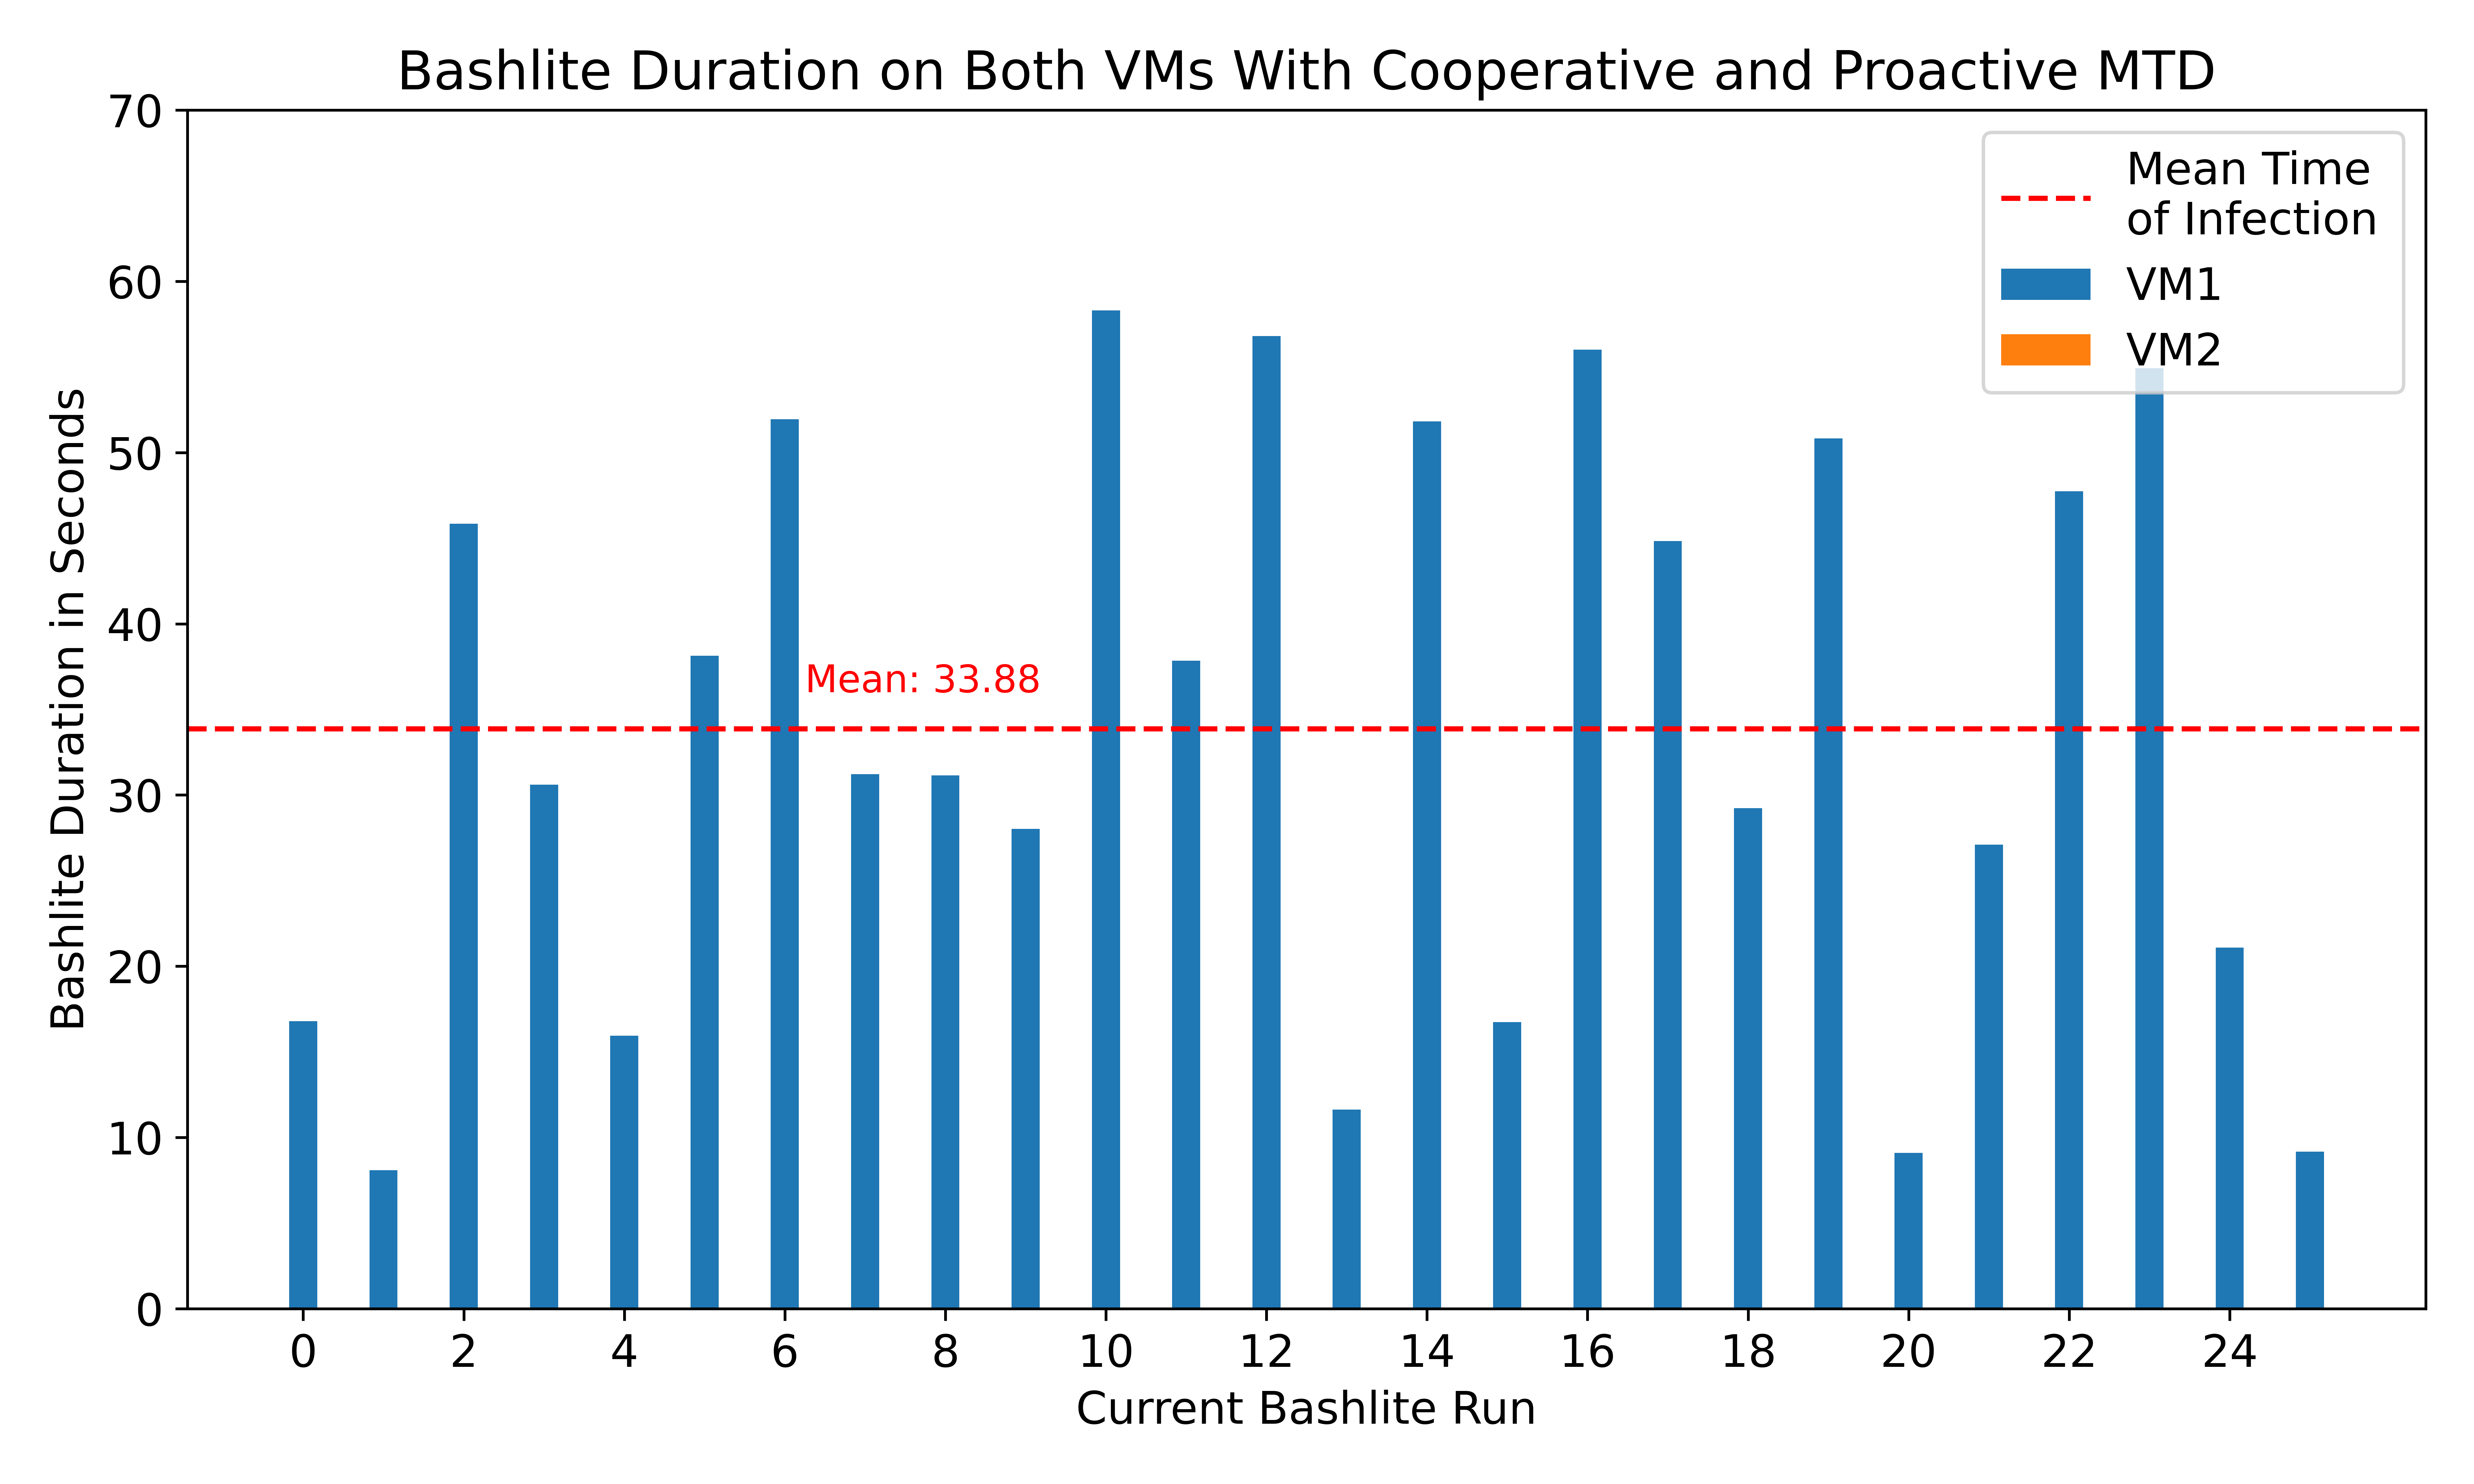
\includegraphics[scale=0.6]{assets/bashliteDurationCoopAndProactive.png}
\centering
\caption{The Duration of Infection Activity on Both Virtual Machines in the Cooperative and Proactive Environment.}
\label{graphic:bashliteDurationCoopAndProactive}
\end{figure}


Figure \ref{graphic:bashliteDurationSummary} shows the duration of the average total infection activity on VM1 and VM2 over 25 runs. The cooperative and reactive environment had the shortest duration of infection activity, the cooperative and proactive environment followed immediately and the non-cooperative and reactive environment had by far the longest average duration of infection activity. This was due to the infection of the susceptible machine.

\begin{figure}[tph]
\includegraphics[scale=0.4]{assets/bashliteDurationSummary.png}
\centering
\caption{A Summary of all Three Environments and Their Respective Infection Duration.}
\label{graphic:bashliteDurationSummary}
\end{figure}


\subsection{Interruption of Availability}
Figure \ref{graphic:packetLossSummary} shows the share of packet losses out of the total packets sent by the two VMs in all three environments. Environment 1, which executed the IP address change on both machines on every run due to the uncooperative nature, had the highest packet loss with about 4.2\%, the remaining 95.8\% were successfully delivered. Environment 2, which consisted of the cooperative and reactive MTD, had by far the lowest packet loss with about 2.1\%. Environment 3 with the cooperative and proactive approach had a similar packet loss as Environment 1. 

\begin{figure}[tph]
\includegraphics[scale=0.4]{assets/packetLossSummary.png}
\centering
\caption{A Summary of all Three Environments and Their Respective Average Share of Outgoing Packet Losses From all Packets Sent.}
\label{graphic:packetLossSummary}
\end{figure}

The incoming Telnet connection showed a different picture than the packet losses, as shown in Figure \ref{graphic:telnetToLocalSummary}. Environment 1 had by far the lowest share (4.2\%) of failed incoming Telnet connections of all incoming Telnet connections. This was due to the fact that no Telnet port changes were involved here (only the IP address change). Environment 2 was in the middle with a share of 31.6\% failed incoming Telnet connections and Environment 3 had by far the highest share of failed Telnet connections with 61.4\%. 

In addition to the incoming Telnet connections, the outgoing Telnet interruptions were also measured. It was evident that changing the Telnet port did not interrupt or prevent any outgoing connections. The only time that outgoing Telnet connections were not possible was when the IP address of the device changed. Therefore, the interruption of outgoing Telnet connections was the same as the share of outgoing packet losses shown in Figure \ref{graphic:packetLossSummary} for every environment. This means that in the non-cooperative and reactive environment
and the cooperative but proactive environment, approximately 4.2\% of outgoing Telnet connections failed. In the cooperative and reactive environment, around 2.1\% of outgoing Telnet connection failed.



\begin{figure}[tph]
\includegraphics[scale=0.4]{assets/telnetToLocalSummary.png}
\centering
\caption{A Summary of all Three Environments and Their Respective Average Share of Failed Incoming Telnet Connections.}
\label{graphic:telnetToLocalSummary}
\end{figure}



\subsection{CPU and RAM Usage}

Figure \ref{graphic:RAMUSageBoth} shows the constant RAM usage of the MTD mechanism over 30 minutes with the MTD techniques executed multiple times on both VMs. VM2 used a minimal amount more RAM, but this difference is negligible as it is in the byte range and the machines have gigabytes of available RAM. So in general, the mechanism's RAM usage was minimal.  

\begin{figure}[tph]
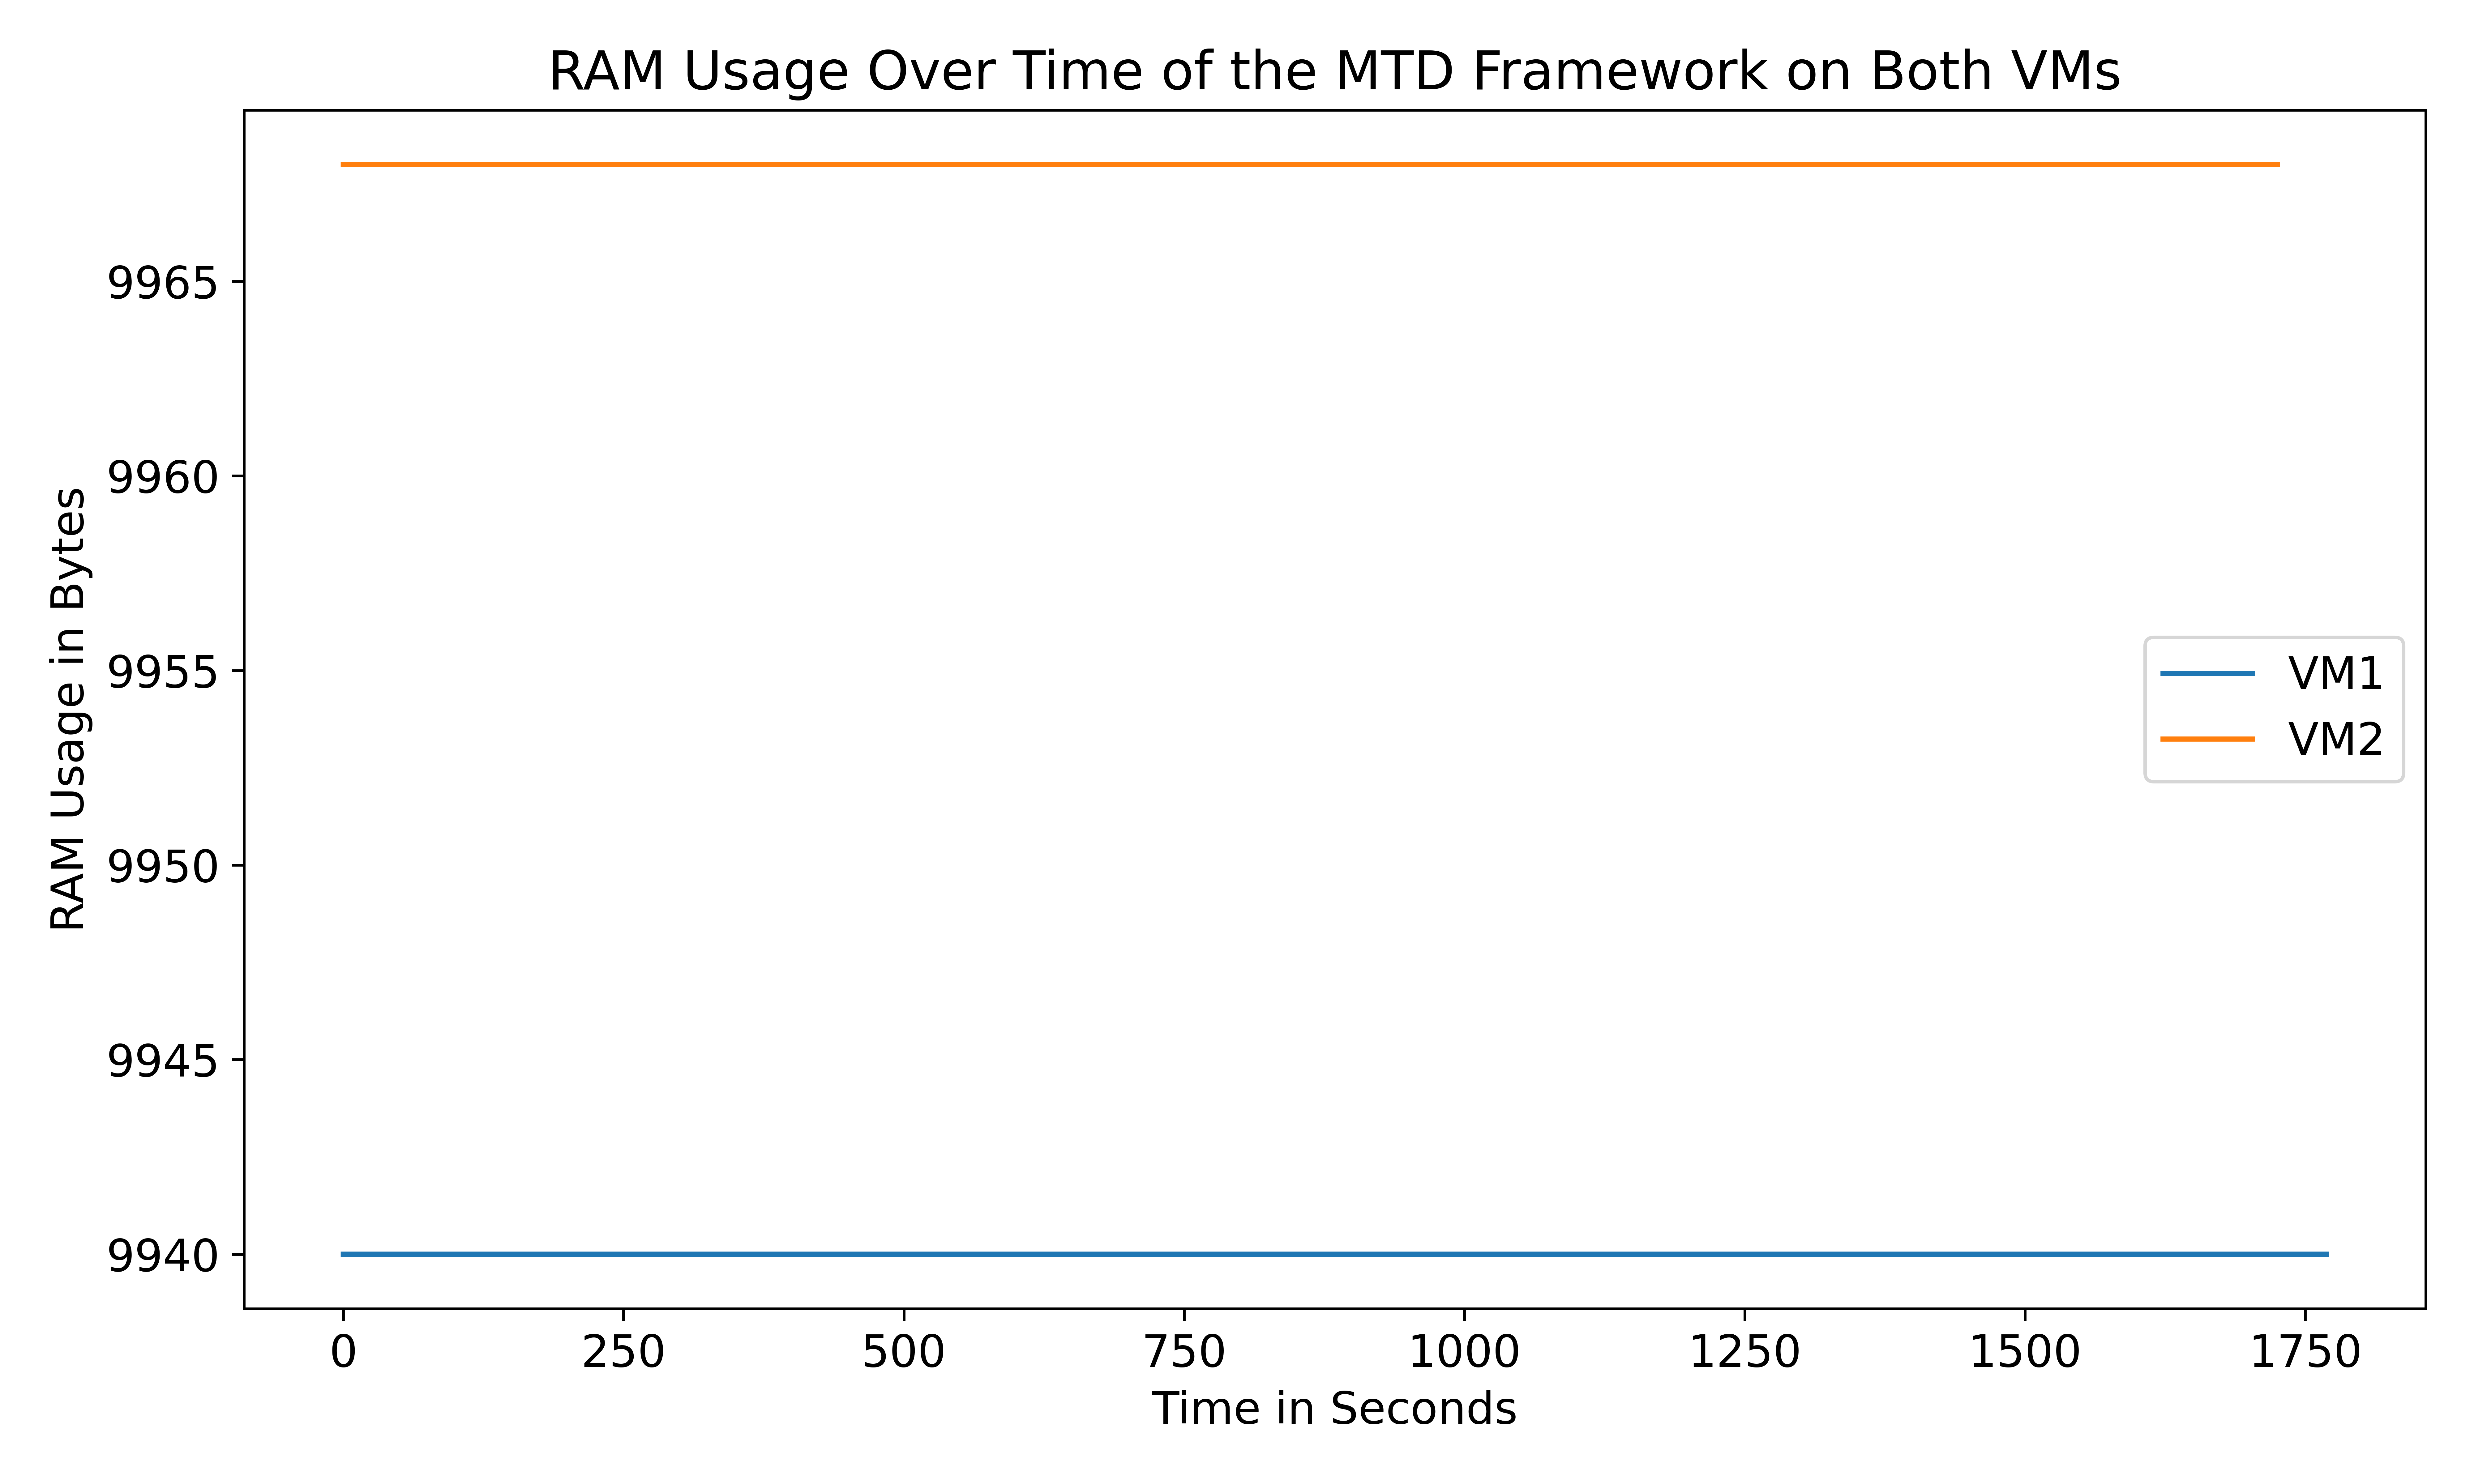
\includegraphics[scale=0.65]{assets/RAMUSageBoth.png}
\centering
\caption{The RAM Usage of the Running MTD Framework with Multiple Executions of the MTD Techniques on Both VMs.}
\label{graphic:RAMUSageBoth}
\end{figure}


Figure \ref{graphic:CPUVM1MTDNotDeployed} shows the CPU usage of VM1 without the MTD deployed. The CPU usage varied between 20\% and 32\% with only a few outliers that are higher. In this case, no other program or script was started except the measurement script, so these outliers must be caused by the operating system or some other automatically started process. The average CPU usage was 23.53\%. Figure \ref{graphic:CPUVM1MTDDeployed} shows the same information, but this time with the MTD framework deployed and the MTD techniques executing multiple times. On VM1 the MTD technique performed was the IP address change. It is clear that the fluctuation was higher with the MTD framework deployed, ranging from 20\% to about 40\%. The high peaks were periodic, but also rather short. The average CPU usage was 0.02\% higher with the MTD mechanism deployed than without it. 

Figure \ref{graphic:CPUVM2MTDNotDeployed} and Figure \ref{graphic:CPUVM2MTDDeployed} give the same information, but for VM2, which performed the Telnet service port change. Again, there was a range of 20\% to 30\% with a few higher outliers in the base case. The average was 23.79\%, which was slightly higher than the average CPU usage of the base case of VM1. The CPU usage of VM2 with the MTD framework deployed and the techniques executing also showed more fluctuation than the base case of VM2. The average CPU usage of the deployed case was also slightly higher, namely 0.43\%. Although there were fewer high peaks on VM2 with the MTD mechanism deployed than in the respective case of VM1, the average CPU usage was higher on VM2 than on VM1.
\begin{figure}
     \centering
     \begin{subfigure}[b]{0.8\textwidth}
         \centering
         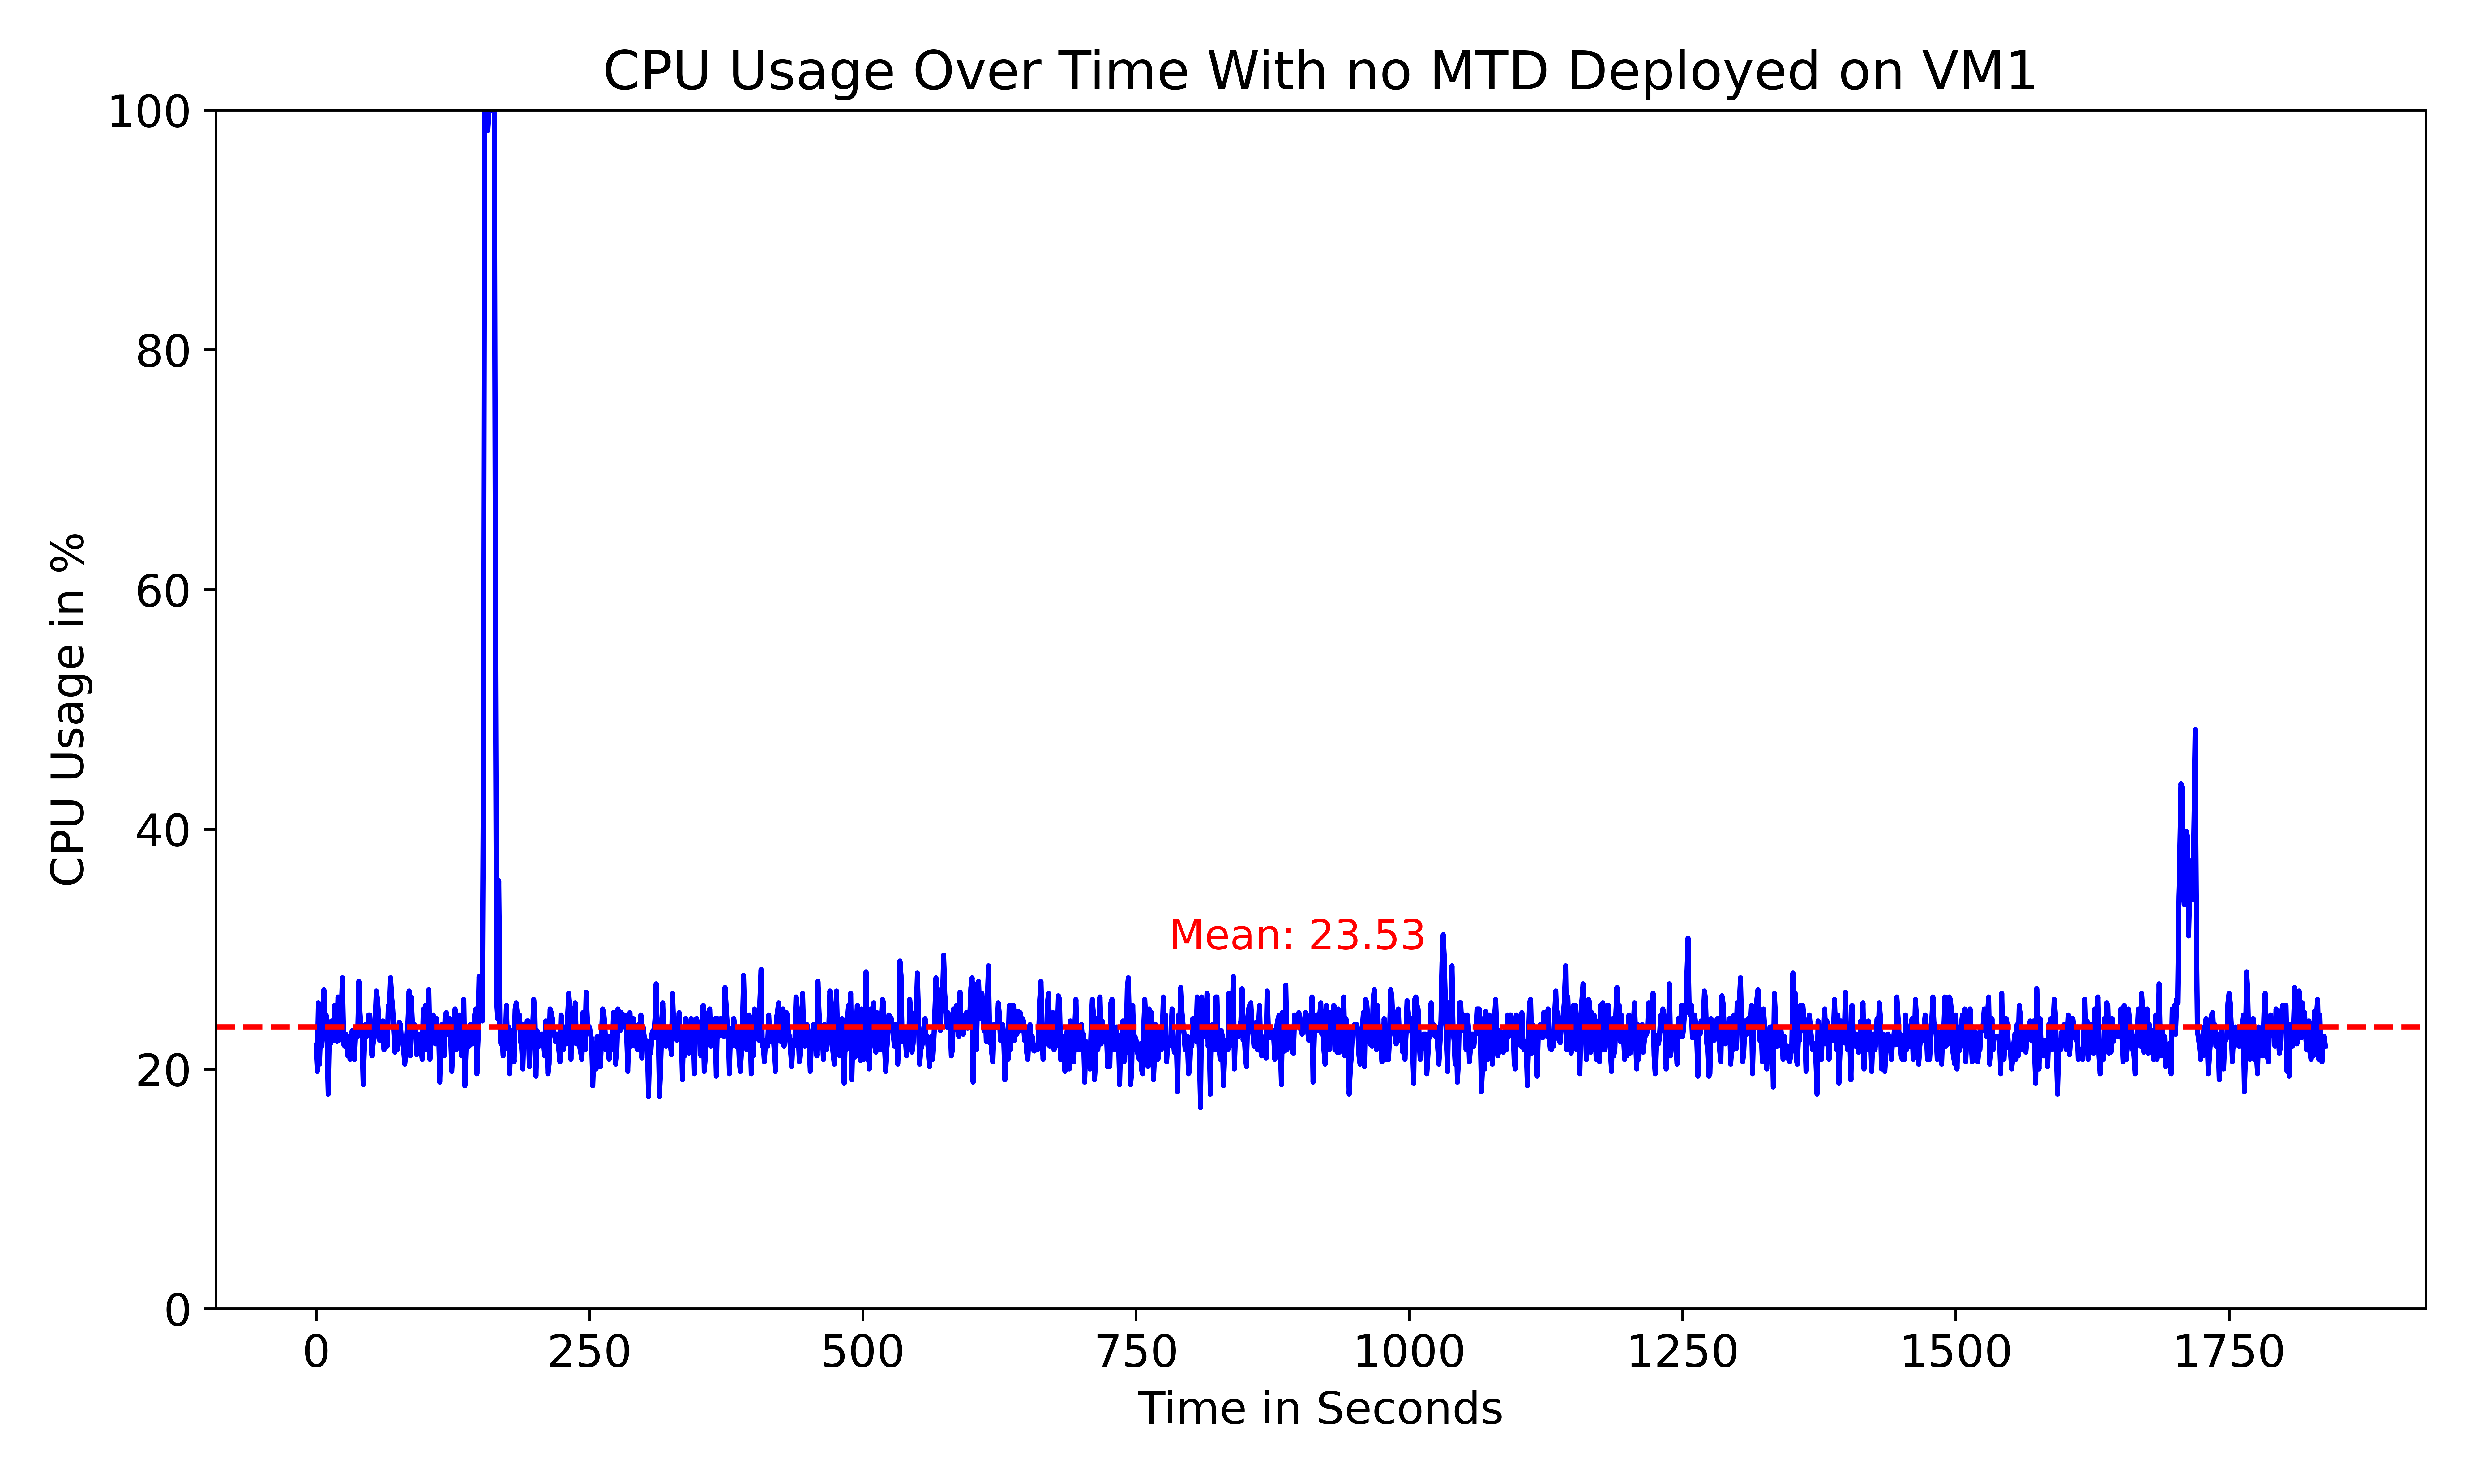
\includegraphics[width=\textwidth]{assets/CPUVM1MTDNotDeployed.png}
         \caption{The CPU Usage of VM1 Without the MTD Mechanism Deployed.}
         \label{graphic:CPUVM1MTDNotDeployed}
     \end{subfigure}
     \hfill
     \begin{subfigure}[b]{0.8\textwidth}
         \centering
         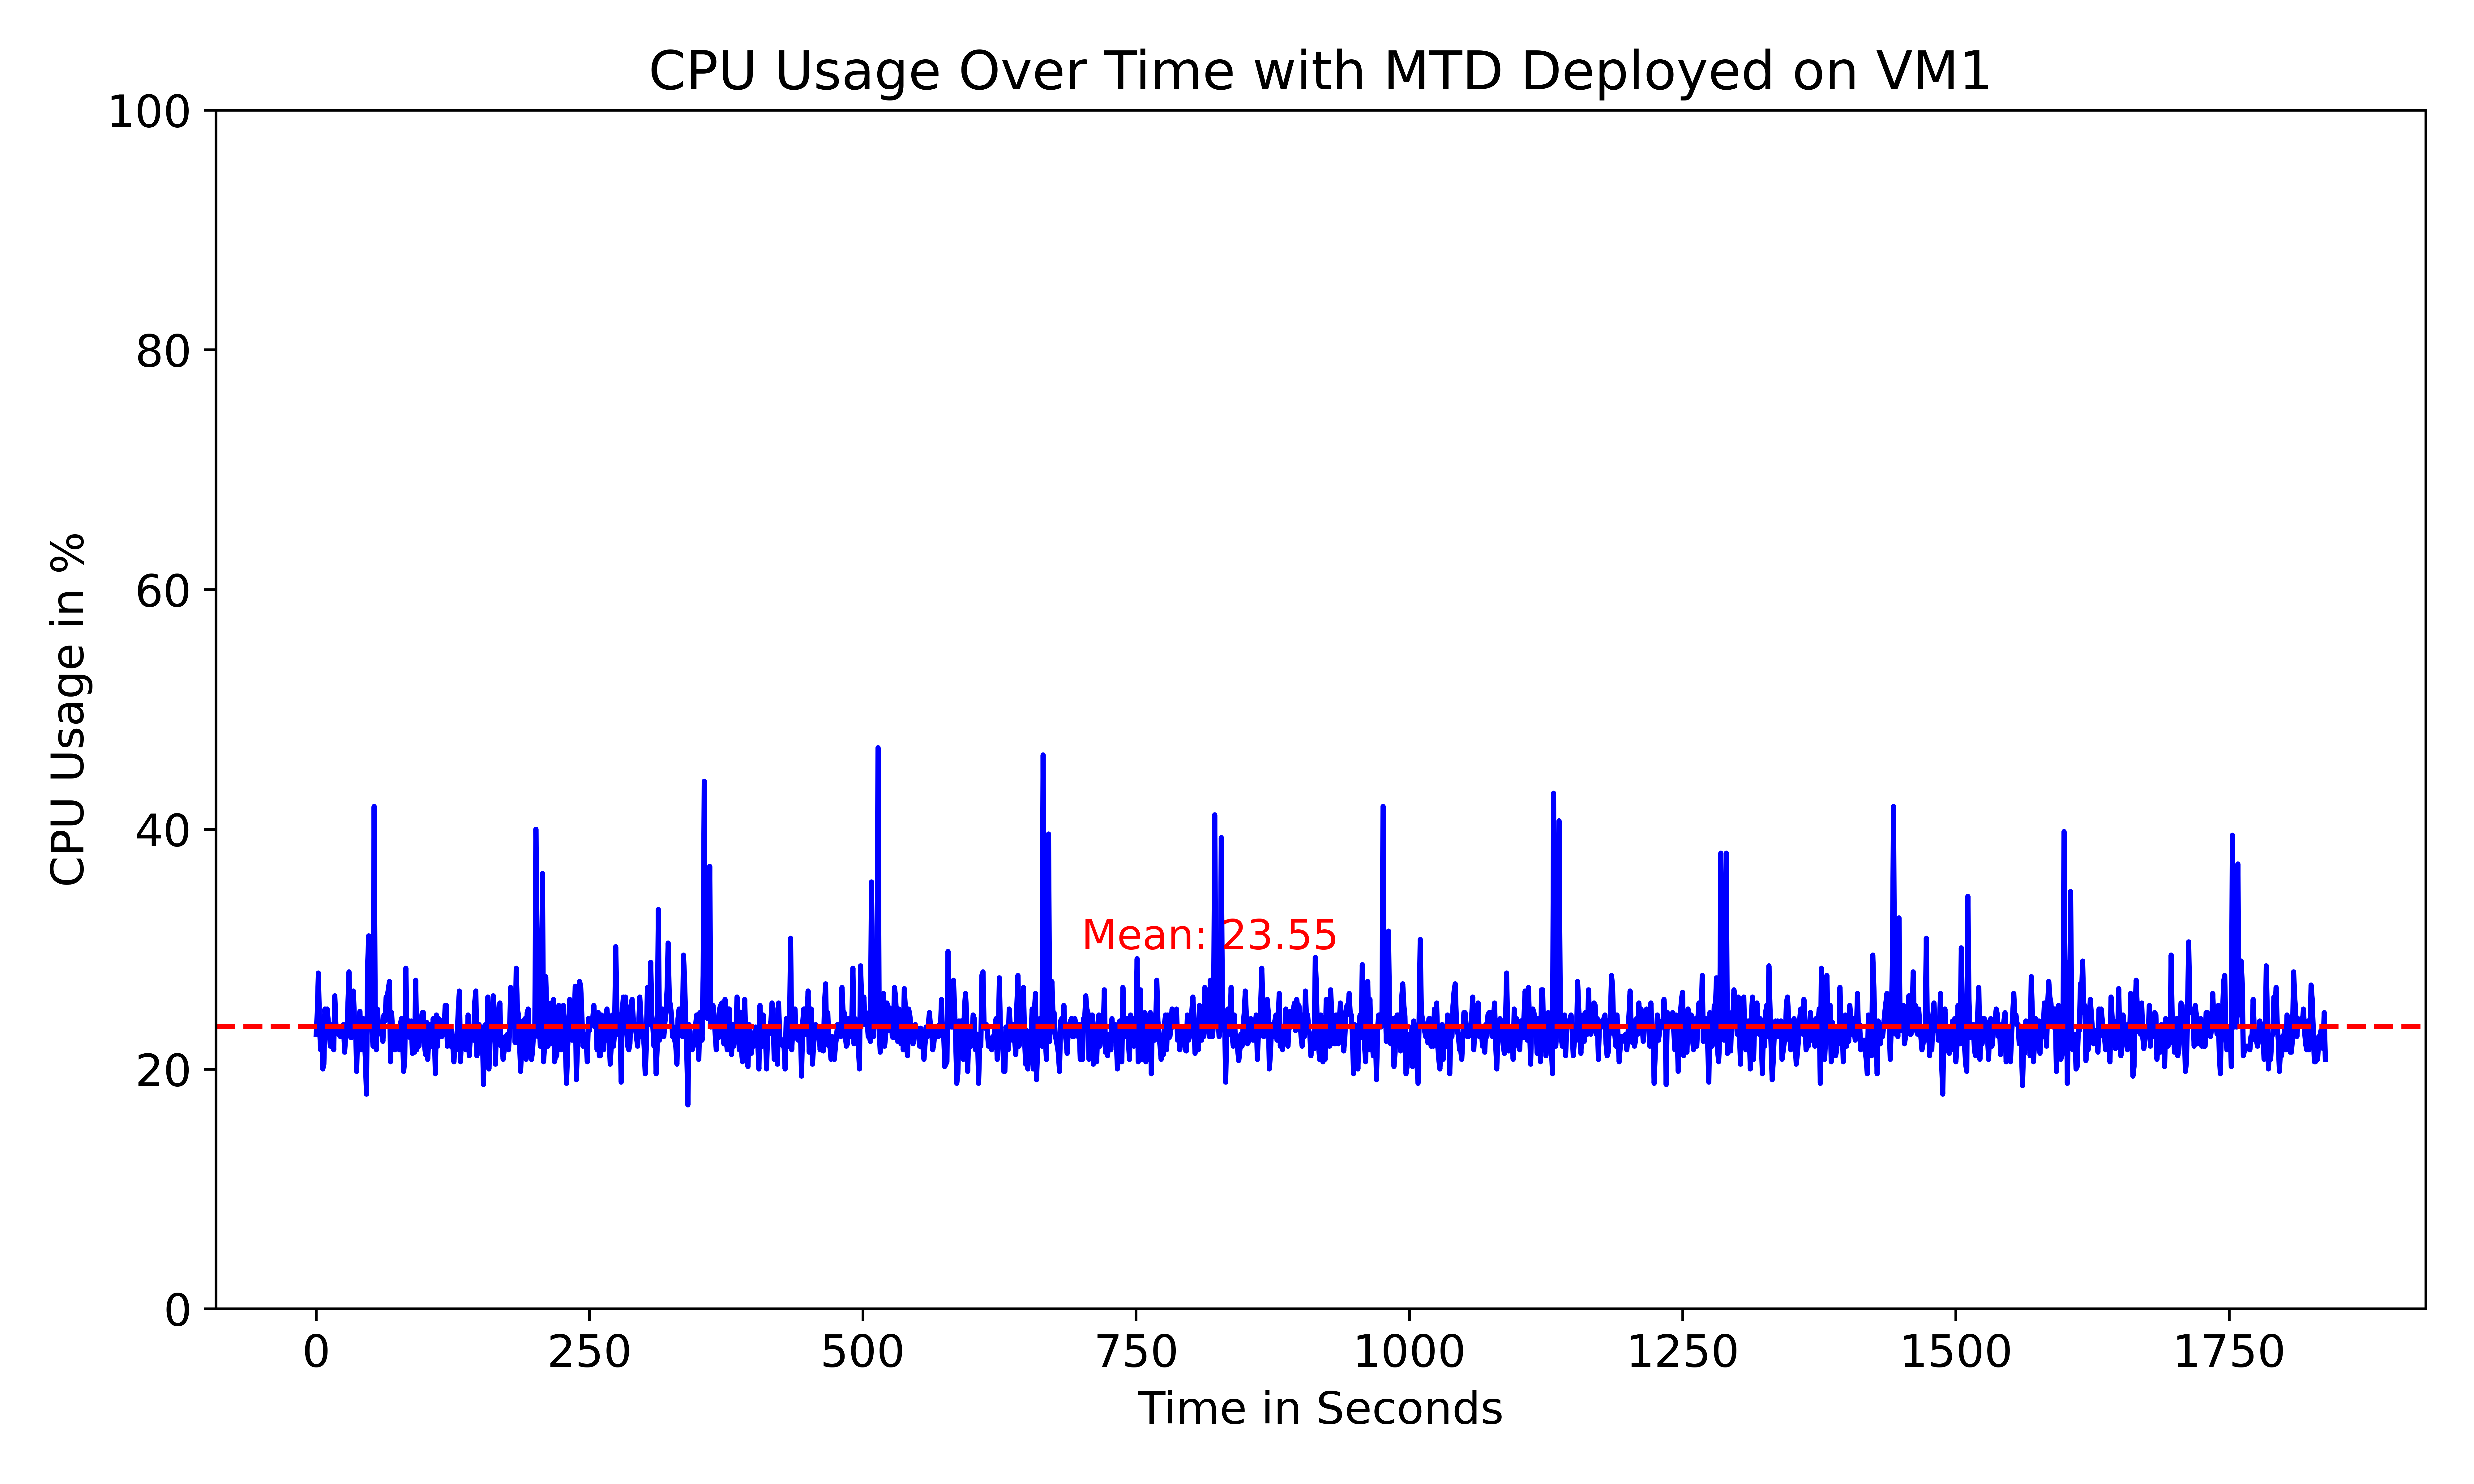
\includegraphics[width=\textwidth]{assets/CPUVM1MTDDeployed.png}
         \caption{The CPU Usage of VM1 With the MTD Mechanism Deployed. This Machine Executed the IP Address Change.}
         \label{graphic:CPUVM1MTDDeployed}
     \end{subfigure}
    \hfill
\end{figure}


\begin{figure}
     \centering
     \begin{subfigure}[b]{0.8\textwidth}
         \centering
         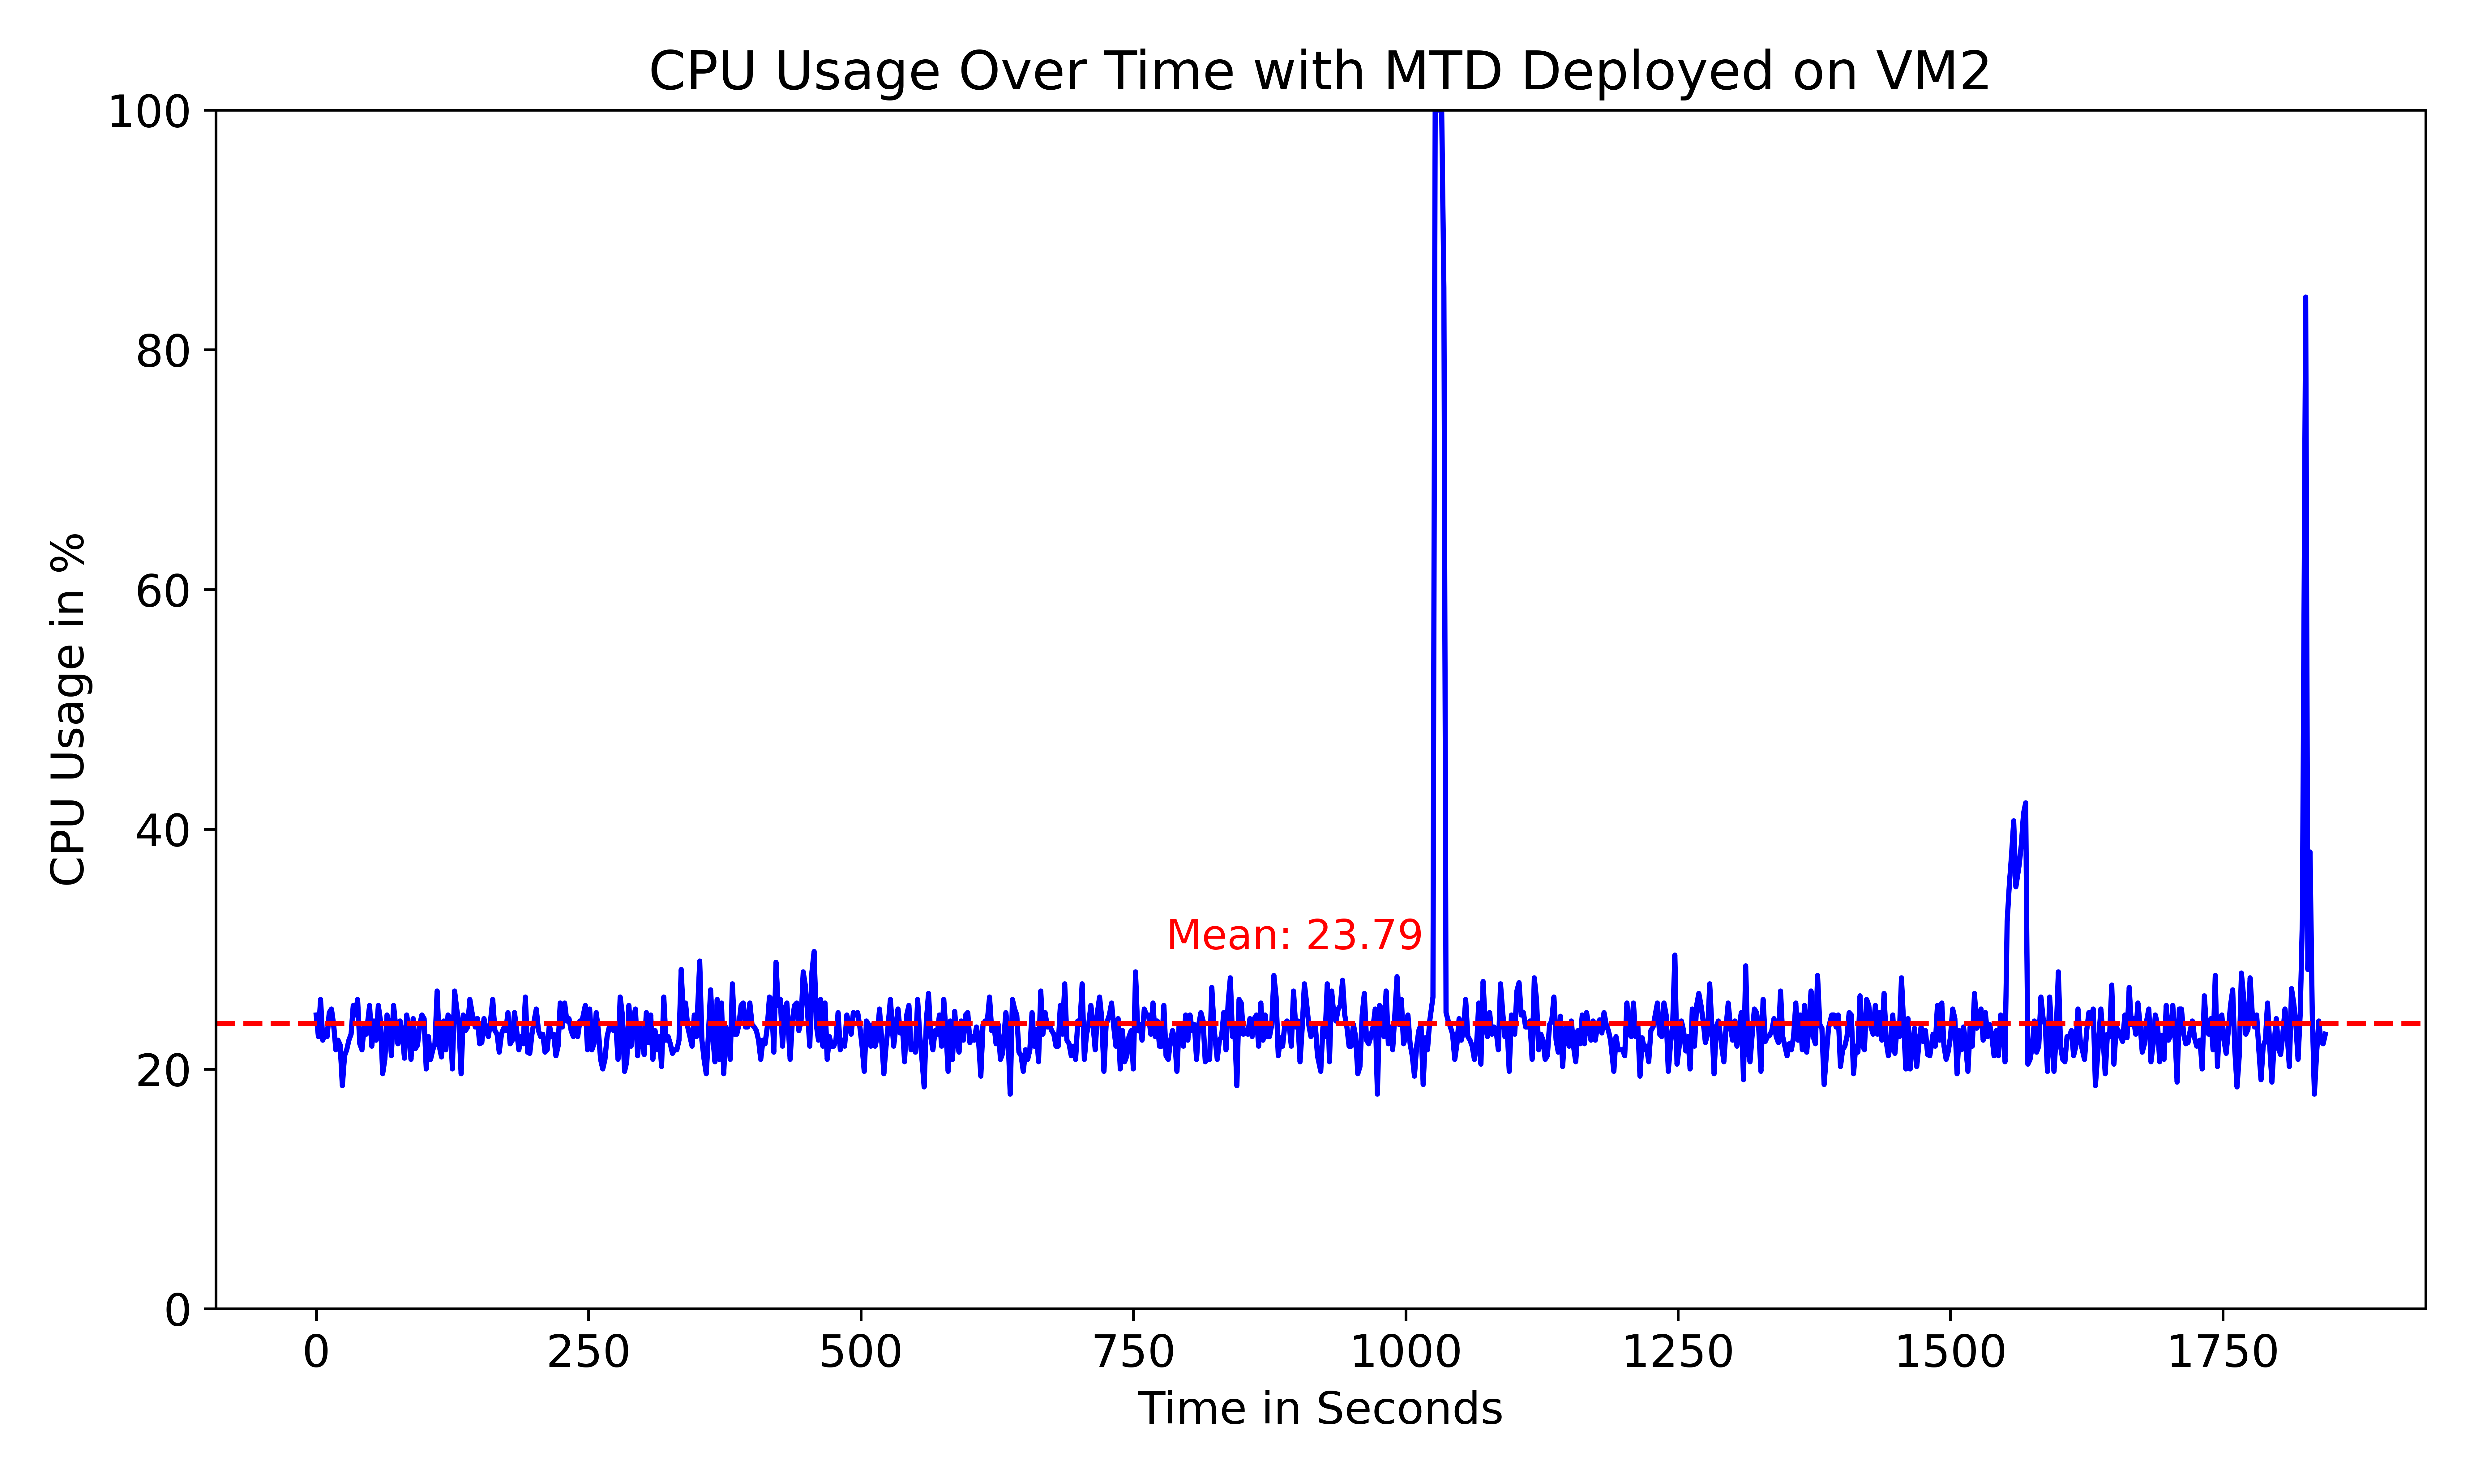
\includegraphics[width=\textwidth]{assets/CPUVM2MTDNotDeployed.png}
         \caption{The CPU Usage of VM2 Without the MTD Mechanism Deployed.}
         \label{graphic:CPUVM2MTDNotDeployed}
     \end{subfigure}
     \hfill
        \begin{subfigure}[b]{0.8\textwidth}
         \centering
         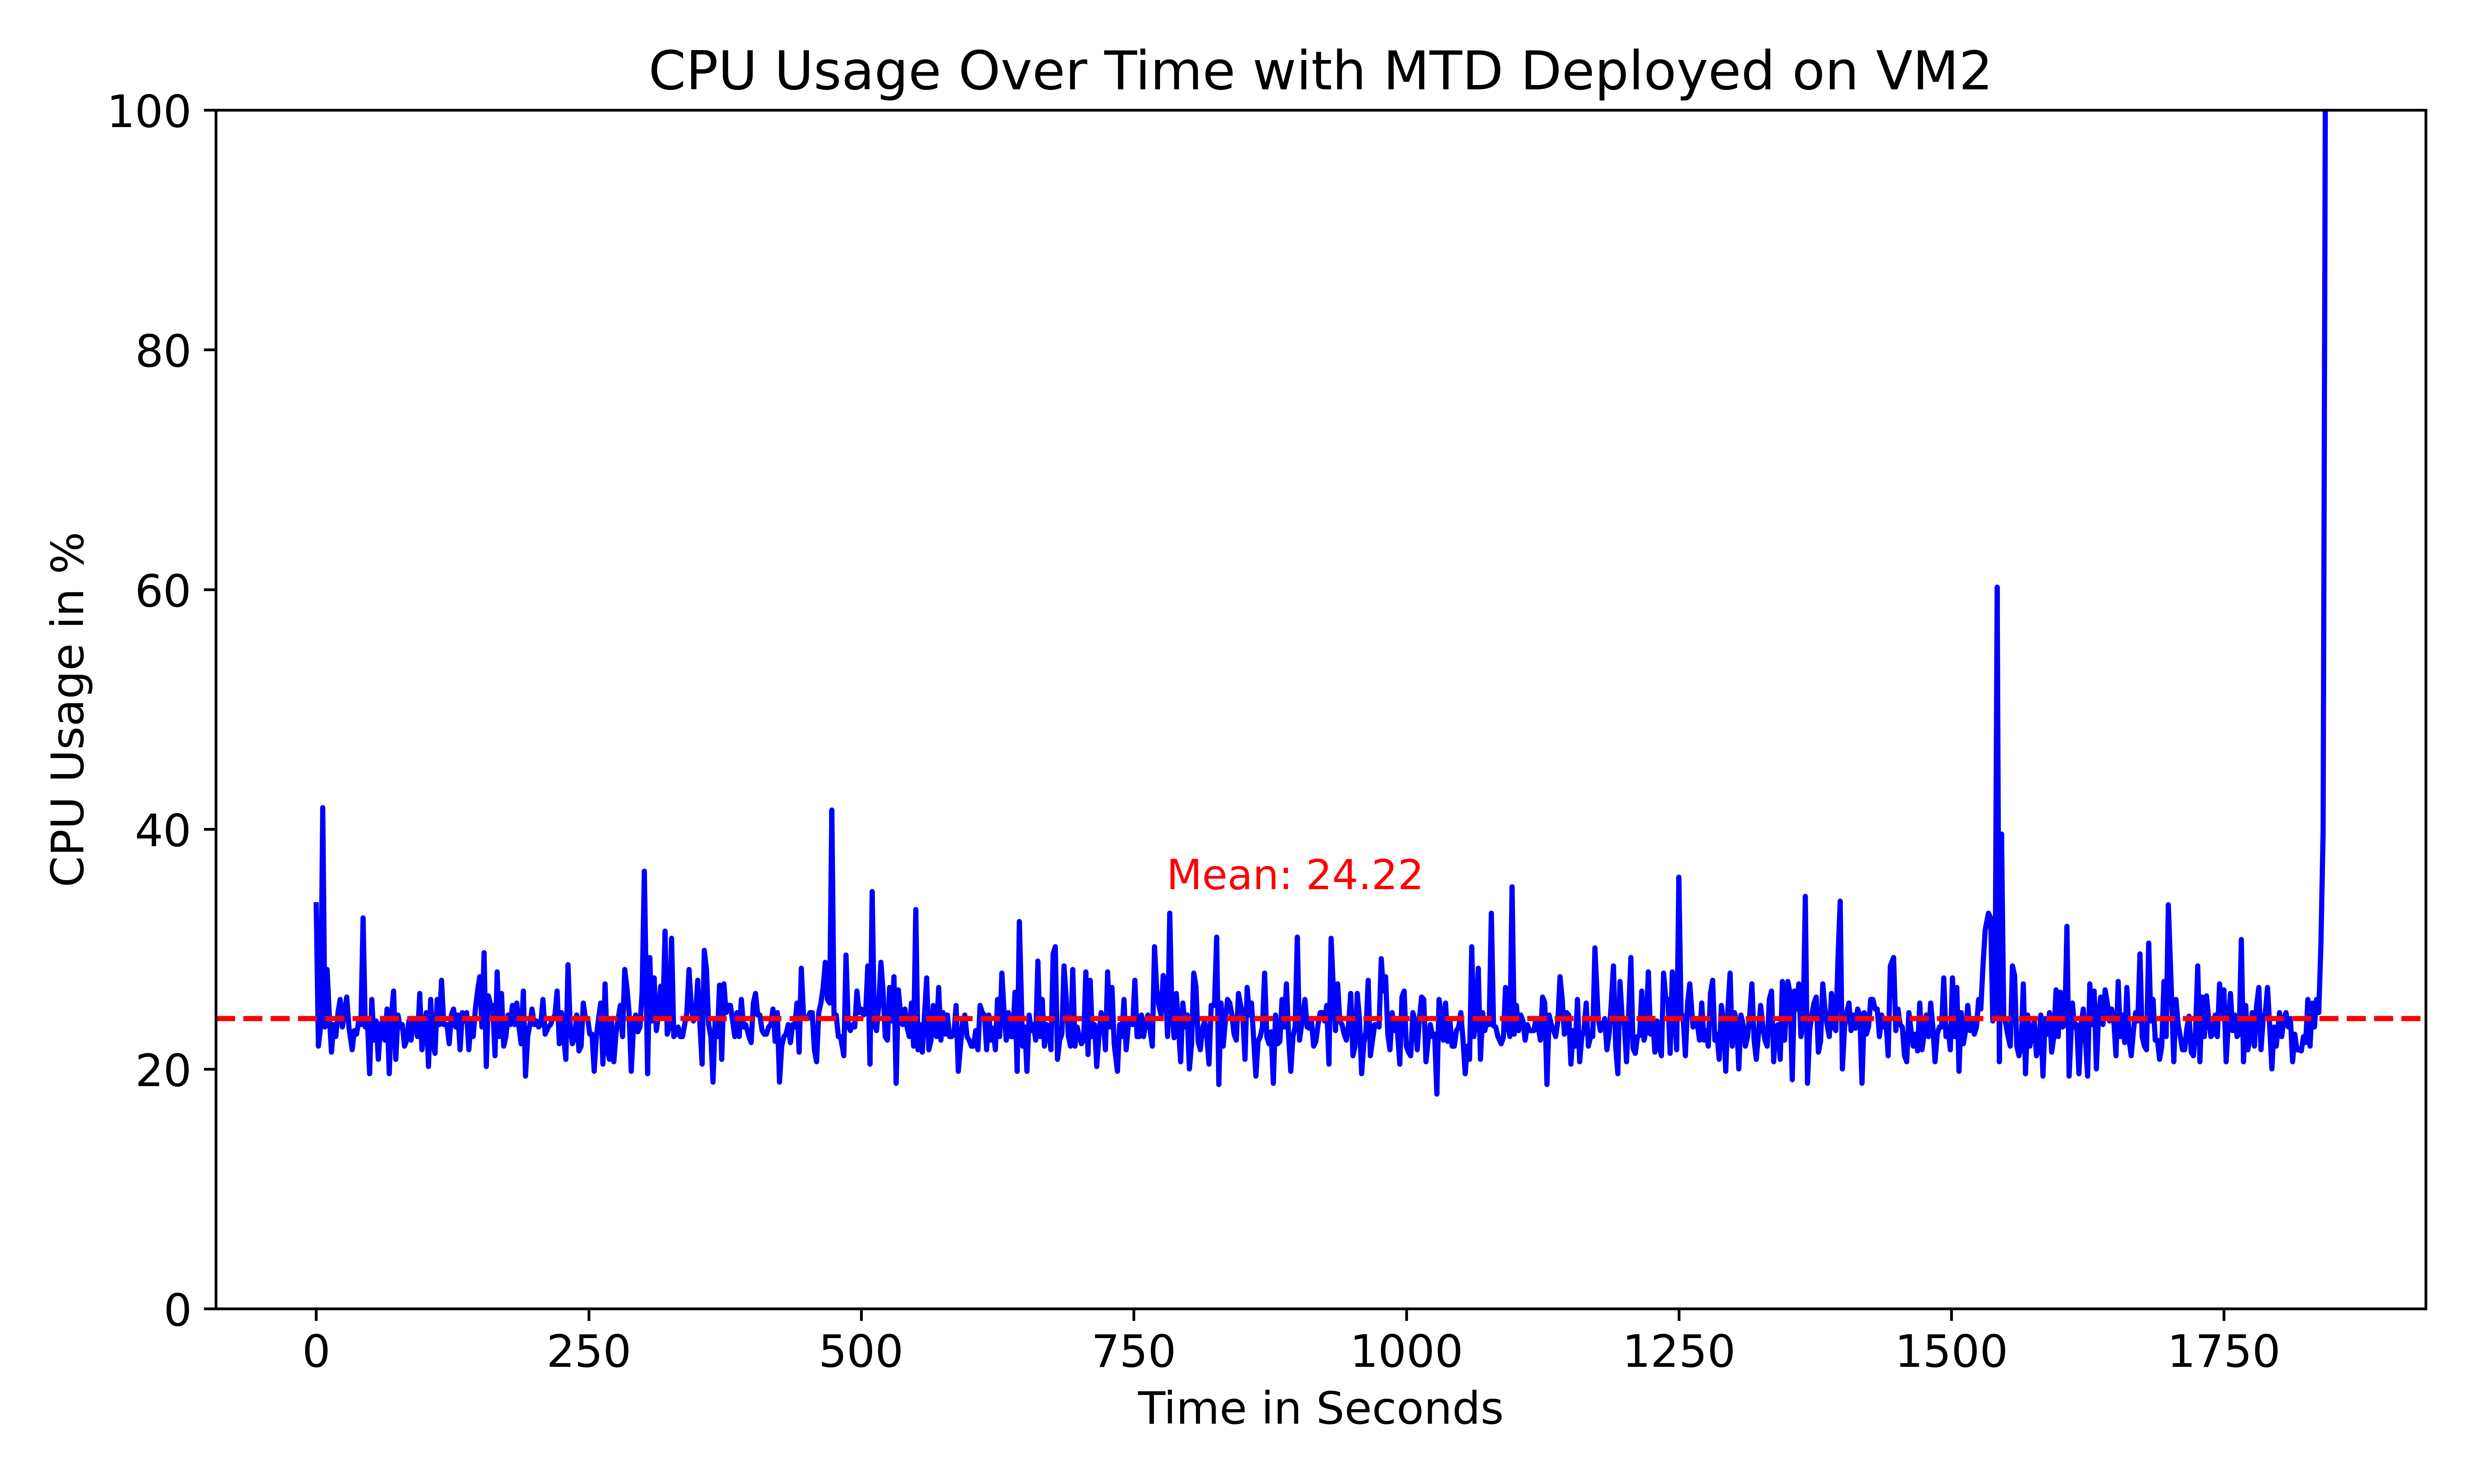
\includegraphics[width=\textwidth]{assets/CPUVM2MTDDeployed.png}
         \caption{The CPU Usage of VM2 With the MTD Mechanism Deployed. This Machine Executed the Telnet Service Port Change.}
         \label{graphic:CPUVM2MTDDeployed}
     \end{subfigure}
     \hfill
\end{figure}



\chapter{Discussion} \label{chapter:discussion}
This chapter presents the discussion of the results shown in Section \ref{section:results}. Additionally, some of the limitations of the thesis are outlined.


\section{Interpretation of Results}
The results of the evaluation turned out as expected. The cooperative and reactive approach provided the best defence against Bashlite, as the overall infection activity was the shortest. It also made sense that the variance of the Bashlite durations was so low in the reactive approaches, because there is no stochastic process involved in the defence mechanisms. In contrast, the proactive environment involves randomness, resulting in different overall infection times for each run. Thus, as long as the MTD techniques execution is reactive and the hardware does not reach its limit, which is unlikely, the mitigation process will have a similar mitigation time for each run. 

This mitigation time was around 29 seconds in the evaluation, which was surprisingly high. 10 seconds are needed for detection~\cite{article:vonderAssen}, the remaining 19 seconds are needed for the mitigation process. A large part of these 19 seconds was caused by the \textit{nmap} scan on the \textit{MTD Deployer Server}. Minimising this scan time was beyond the scope of this thesis, but it would be achievable~\cite{website:nmapTiming} and should be implemented in a more sophisticated solution. Another convenient way to reduce the \textit{nmap} search time would be to change the range of possible IP addresses in the \textit{MTD Deployer Server} configuration file. The evaluation was done with a range of 90 IP addresses, whether this is a reasonable number depends on the system in which the MTD would be deployed.

The detection time is another crucial variable. In this thesis, a detection time of around 10 seconds was used, as it was shown that Bashlite could be detected in this time~\cite{article:vonderAssen}. If this time were longer (e.g. with another malware), it is possible that a reactive approach would not be able to prevent the malware from spreading. This could force a user to use a proactive defence mechanism instead of a reactive one. The proactive approach used in the evaluation was successful in preventing Bashlite from spreading to the susceptible machine with the variables selected. This is by no means certain. Several variables are decisive whether the spreading of Bashlite can be prevented, the most important ones are: the time interval after which Bashlite is executed randomly, the execution interval of the MTD mechanism, and the time after which the Telnet service port is moved back to port 23. 

If the system protection was the only criterion, it would be best to run the MTD techniques at a very short interval. For example, an MTD mechanism (e.g. IP address change) executed every second would result in an extremely short overall infection activity. While this is desirable, it is not feasible as the connections to and from the device would always be interrupted, defeating the purpose of the device (e.g. a sensor collecting data). Thus, there is usually a trade-off between system availability and security. 

This trade-off between availability and security was also reflected in the results. In terms of outgoing packet losses, the non-cooperative and reactive approach had the highest share of packet loss out of the total number of packets sent. This is evident as both machines had to change their IP addresses, which is the cause of the packet loss. 

The share of failed packet losses can also be approximated mathematically. In this non-cooperative and reactive environment, a run took 120 seconds on each machine, resulting in a total of 240 seconds in the system. Restarting the Ethernet adapter to force the machine to use the new IP address takes about 5 seconds per machine, making a total of 10 seconds. 10 seconds is about 4.2\% of 240, which is the approximate interruption percentage. This also explains why the packet loss share of all packets sent in the cooperative and reactive environment was exactly half of the packet loss in the non-cooperative and reactive environment. Again, the total time was 240 seconds, but this time only one machine changed its IP address. 5 seconds out of 240 seconds is 2.1\%. The same calculations can be done for the cooperative but proactive environment. Here only one machine had to change its IP address, but it did so every 60 seconds due to the proactive approach. As there are two machines again, this gives a total of 120 seconds in the system. 5 seconds is about 4.2\% of 120 seconds. 

So far, the cooperative and reactive approach performed best. This approach had the lowest total infection time and the lowest share of outgoing packet losses. This was different when looking at the share of failed incoming Telnet connections. Here the non-cooperative and reactive approach performed best. This is evident as this approach did not initiate port changes, which are the main cause of failed incoming Telnet connections. Although not clearly visible in the figures, the share of failed incoming Telnet connections for this non-cooperative and reactive environment is identical to the share of its packet loss (4.2\%). This is due to the reboot of the Ethernet adapter, as a working IP address is a prerequisite for successful Telnet connections. 

The cooperative and reactive environment had a much higher interruption share of incoming Telnet connections due to the moved Telnet service port. It is important to note that this share was heavily influenced by the defined time to switch back to port 23, which can be specified in the \textit{MTD Deployer Server} configuration file. The 30 seconds selected for the evaluation were chosen because Bashlite would definitely be rendered harmless on the infected device and the port could therefore be moved back after 30 seconds. Again, the share of failed incoming Telnet connections was twice as high in the cooperative but proactive environment as in the cooperative and reactive environment. This is because the former ran the MTD every 60 seconds and the latter every 120 seconds. 



As mentioned earlier, there is a trade-off between security and availability and all the deployment strategies had their advantages. However, the only advantage that the non-cooperative reactive system had over the cooperative reactive system is the lower rate of failed incoming Telnet connections. Although it is unlikely that the availability of a device's Telnet port is more important than security and the outgoing packet loss rate, a solution in this case would be to use an uncooperative defence.

The cooperative and reactive approach also showed better results in the evaluation than the cooperative but proactive approach. However, this case is more complex as it depends on various factors such as the detection time of the malware or again the trade-off between security and availability. The proactive approach could theoretically provide better security results than the reactive approach, but this would also increase the interruption of the services. In a real system, the requirements of the underlying system would have to be compared with the advantages and disadvantages of the MTD solution. One way of doing this is to calculate the interruption time and decide which approach is more suitable for the system at hand. 



%As the results showed, the cooperative and reactive approach can definitely be a powerful tool against IoT malware. It significantly reduced the overall infection activity on a system and also had some advantages in terms of interruption of machine availability compared to an non-cooperative and reactive approach. The evaluation was done with only one susceptible machine, the difference would be even more significant with more than one susceptible machine in the network. In general, it is important to note that each deployment strategy had its advantages. Therefore, it is essential that the underlying system, as well as the possible threats to the system, are analysed prior to any potential real-world deployment to determine which approach provides the best overall solution with the fewest downsides.
In general, the cooperative and reactive approach can be recommended for most systems, as this will only run the MTD techniques if Bashlite has been found on the system. This avoids unnecessary interruption of the system that would occur with the proactive approach. However, it is impossible to make a final statement, as the choice also depends on the malware. If a really aggressive malware is trying to infect and possibly destroy the devices, a proactive approach may still be more reasonable. Nevertheless, the possibilities offered by a cooperative defence mechanism are very promising. 

Even in case a proactive approach is the required solution, there is no need to worry about the resources of the device, as it was found that the MTD framework and executed techniques used only a minimal amount of hardware resources. This is evident from the fact that it does not take many hardware resources to execute the \textit{sed} command to replace something in a file and then restart either the Ethernet adapter or the \textit{inetutils-inetd} service. The peaks seen in the CPU usage of VM1 with the MTD deployed are almost certainly caused by the restart of VM1's Ethernet adapter. It is not clear what caused the peaks of VM2. The reason may be the restart of the \textit{inetutils-inetd} service, but as they were not as periodic as VM1's peaks, it is difficult to determine.
However, these peaks were extremely short and therefore not a problem even for resource-constrained devices. In terms of RAM usage, the results were similar. The MTD framework and the executed techniques used only about 10,000 bytes of RAM. This is negligible compared to the 3.7 GB the machines had at their disposal, as it is less than 0.0003\%.

The results of this evaluation could also be usefully combined with two of the frameworks presented in Section \ref{section:MTDFramework}. The first was the framework that helps to answer the design questions (What, How, When) for an MTD mechanism. The What and the How are already determined by the implemented MTD mechanism, as well as the When for the reactive case, since this is determined by the detection time. However, the When for the proactive approach could definitely be determined with the help of this framework. The second framework was the IANVS framework, which aims to help implement MTD techniques in distributed systems. Whether this is needed or not depends on the system. As long as the connections of the IoT devices are outgoing and the target is static, such a mechanism is not needed because the IoT device can still connect to the target regardless of what IP address the IoT device currently has. However, if a device needs to connect to the IoT device, such a mechanism needs to be implemented. 




\section{Limitations} \label{section:limitations}
There are some important limitations in several aspects of this thesis. The first is the operating system of the virtual machines. As described, the initial setup was with the Ubuntu operating system, which had to be changed to the Raspberry OS in order to run Bashlite. This change caused the original implementation of the IP address change to fail. Although the Python parts of the solution should work independently of the OS, it is possible that the Bash commands executed in the Python code may need to be adapted on a different OS. This is especially important as there are many different potential operating systems for constrained devices, as shown in Section \ref{sec:hardSoftware}.

Another limitation is the chosen malware. In this thesis, Bashlite was used as the malware to work with. However, there exist more sophisticated malware that may be able to evade the defence mechanisms presented. Although this could only be evaluated through the code on GitHub, a malware such as Mirai has implemented the functionality to reconnect to its server when the client does not receive a response from the server. This makes the IP address change more of a short-term obstacle than a long-term solution. Additionally, it is not entirely clear how the IP address change would perform against a P2P malware such as the HEH malware described in Section \ref{subsection:P2PIoTBotnets}. At the very least, the Telnet port change technique is, in theory, a well working defence against malware such as HEH or Mirai. However, this also needs to be thoroughly tested in practice. Additionally, it is worth noting that malware can also target a device's SSH port. This thesis has only focused on the Telnet port.    

As already described in more detail in the previous Chapter (\ref{chapter:discussion}), the results of the evaluation were strongly influenced by the chosen variables and the configuration file (e.g. the proactive execution rhythm or the IP address range to be scanned by \textit{nmap}). Although this is normal in such an evaluation, it is important to emphasise this when talking about the limitations. Even though the variables selected for this thesis were carefully chosen, it is not possible to draw an absolute conclusion from the result. It is clear that in most cases it makes sense to use a cooperative and reactive approach where possible, but there may be environments/systems where the  cooperative and proactive approach is more suitable. Various variables determine how well an MTD approach performs, and different MTD approaches may have different advantages and disadvantages. It is therefore important to tailor the chosen MTD approach to the requirements of the system that is to be protected by the MTD solution.



\chapter{Conclusion}
This thesis proposed and implemented a cooperative Moving Target Defence (MTD) framework for IoT devices along with two MTD techniques. IoT devices are inherently susceptible to malware for several reasons, including poor maintenance and neglect of security \cite{article:DDoSinIoT}. This insecurity, combined with the immense number of existing IoT devices \cite{website:statistaIoT}, makes these devices a popular target for malware. Infected IoT devices can be used for various malicious behaviours, the most common use case being botnets to perform DDoS attacks, for example. One way to defend IoT devices against malware is MTD, that attempts to change the attack surface of a system to defend it against attackers \cite{navas:2021MTDWhere}. \cite{article:vonderAssen} showed that it is possible to disconnect a Bashlite bot from the Bashlite server by changing the private IP address of the client. The solution proposed in this thesis builds on this by adding a cooperative component, as this provides a significant advantage to the defence mechanism.

In order to find an effective defence, a suitable malware had to be found. The choice fell on Bashlite, a fairly well-known IoT malware. Even though Bashlite was available on code repositories, some adaptations had to be made to the code to provide, among other things, the spreading functionality. With Bashlite working, the cooperative MTD mechanism could be developed. As a test bed, three virtual machines running Raspberry OS were used, one as a server machine and the other two to mimic the IoT devices. Of these two mimicking machines, one was manually infected (VM1) and the other was the susceptible machine (VM2) that was eventually infected through the spreading of Bashlite. 

The implemented solution consists of two different MTD techniques, which are the IP address change and the Telnet service port change, as IoT malware often infects devices via Telnet. The currently infected device performs an IP address change to disconnect itself from the Bashlite server, making communication with the server impossible. All other devices in a given IP address range should change their Telnet service port for a specified time to hide from Bashlite.

After the implementation, the solution was evaluated using several metrics, including the overall infection time of Bashlite on the two virtual machines, the network interruption caused by the execution of the MTD, and the RAM and CPU usage. These three metrics were measured in three different environments for comparison. The first environment was an non-cooperative and reactive MTD approach. This environment executed the MTD techniques 10 seconds after Bashlite was detected, but did not include a cooperative component. This means that Bashlite first had to be detected on the machine in order to disrupt its connection to the Bashlite server. The second environment was a cooperative and reactive MTD approach. Again, the MTD techniques were executed 10 seconds after Bashlite was detected, but here with the cooperative component. This was the solution developed in this thesis. The third and final environment was a cooperative but proactive environment. This was used for comparison and to show the trade-off between a proactive and a reactive MTD approach. This proactive approach ran the MTD techniques after a specified time interval (1 minute), regardless of whether Bashlite was on the system or not. 

The results showed that in the non-cooperative and reactive approach, the susceptible machine was infected on every run of Bashlite. This meant that both machines had to change their IP address to disconnect from the Bashlite server, resulting in each machine being infected for approximately 29 seconds. The cooperative and reactive approach completely prevented the spreading of Bashlite to the susceptible machine by changing the Telnet service port of the susceptible machine. Therefore, only the manually infected machine was infected for 29 seconds and the susceptible machine was not infected at all. This meant that the overall duration of infection activity on the two VMs was halved. Although not tested, this would be even more significant with more susceptible machines, as any infection other than the first could be prevented. Finally, the cooperative but proactive approach also prevented Bashlite from spreading to the vulnerable machine with the chosen configuration. However, it also showed a large variance in Bashlite duration on the first machine, as randomness partly determines after what time the MTD techniques are initiated. This resulted in an average Bashlite duration of 34 seconds on VM1 and 0 seconds on VM2. The results of this approach are strongly influenced by the configuration chosen, i.e. the interval at which the MTD techniques are initiated and other variables. It is also possible, for example, that the spreading of Bashlite cannot be prevented at all if the interval between the execution of the MTD techniques is too long.

Besides the overall infection time, the downtime of the machines is an important metric. The results clearly showed that a cooperative and reactive approach gave better results in terms of downtime than the uncooperative and reactive approach, as long as Telnet is not required on the susceptible machine. The cooperative and reactive approach also caused much less downtime (about 50\%) than the proactive and cooperative approach, which was to be expected. The final metric was the CPU and RAM usage of the MTD techniques. It turned out that both machines used on average a maximum of 0.43\% more CPU with the MTD mechanism deployed than without it and that the RAM usage of 10000 MB on each machine was negligible. 

Although the cooperative and reactive approach performed best in the evaluation, the other approaches should also be kept in mind. This is due to the different variables that should be considered when deciding on the most suitable MTD approach. Each approach has different advantages and disadvantages. For example, a short-interval proactive approach may be the best solution if the overall infection time of the system is to be minimized, and high downtime of connections to and from the machines is not an issue. In addition, it may be that the malware in question is not (yet) detectable, in which case the proactive approach would be required anyway.
However, for most systems, the cooperative and reactive approach will provide the best overall solution.

With the threat of IoT malware increasing both in number \cite{website:KasperskyAMalwareStory} and with new highly dangerous variants such as P2P malware \cite{website:trendMicroUncleanable}, it is essential to have the best possible defence options. One of these options is the Moving Target Defense which has proven to be a promising defence strategy for IoT devices, especially when it includes a cooperative component, as shown in this thesis. To be prepared for future threats and especially against P2P malware, further research on how cooperative Moving Target Defense can defend against IoT malware is essential.


\section{Future Research} \label{section:futureResearch}

As the topic of MTD is large and complex, there are several possibilities for further research. This thesis has shown that the cooperative and reactive MTD approach offers several advantages over other approaches. Examples of these advantages are a comparatively lower duration of infection activity on the system and a comparatively lower interruption of availability. A prerequisite for a reactive MTD approach to work is the ability to detect potential malware on the system. Therefore, research on fast and reliable malware detection mechanisms is essential. One possible means for that are machine learning algorithms~\cite{article:vonderAssen}.

Another research option is to further develop the presented solution. Possible improvements are to make the solution faster, for example by optimizing the \textit{nmap} scan, or to adapt the solution for other operating systems. A significant research would be to investigate if and to what extent the current solution works against malware such as Mirai or P2P botnets. Theoretically, moving the Telnet service port should also protect against these malwares, but this should be tested in practice.       

Another interesting area of research would be to further investigate the impact of the LAN setting. This has only been touched on slightly in this thesis, but the LAN setting could provide additional options for the malware that could have a negative impact on an MTD defence mechanism. For example, one of these potential options are port scanners that might be able to find the moved Telnet port.

Finally, the presented solution uses a classic client-server architecture. This was due to the simplicity provided, which allowed the basic concept of cooperative MTD to be tested more quickly. For a more sophisticated implementation, other architectures should be considered. For example, one option is 
a P2P architecture, which would provide the corresponding advantages, such as e.g. the removal of the single point of failure.





\printbibliography[heading=bibintoc, title={Bibliography}]

\chapter*{Abbreviations}
\addcontentsline{toc}{chapter}{Abbreviations}
\markboth{ABBREVIATONS}{}

\abr{6LoWPAN}{IPv6 over Low power Wireless Personal Area Network}
\abr{MTD}{Moving Target Defense}
\abr{MP}{Moving Parameter}
\abr{OS}{Operating System}
\abr{C\&C}{Command and Control}
\abr{DDoS}{Distributed Denial of Service}
\abr{P2P}{Peer-to-Peer}





\chapter*{Glossary}
\addcontentsline{toc}{chapter}{Glossary}
\markboth{GLOSSARY}{}


\begin{description}
  \item[Moving Target Defense] A cybersecurity paradigm that aims to change the attack surface of a system by altering its properties, such as the IP addresses or the data representation.
  \item[Moving Parameter] The "what" that should be changed as a part of the Moving Target Defense. An example is the value of the IP address. 
  \item[Internet of Things] Items such as sensors that are connected through a network and collect and exchange data.
  \item[Botnet] A collection of bots that are remotely controlled and can be used to launch cyber attacks.
  \item[Bashlite] A well-known IoT malware that was the basis for other well-known IoT malware such as Mirai. Aims to create a botnet of infected devices.
  \item[Mirai] An IoT malware still prevalent today that, like Bashlite, aims to create a botnet of infected devices.
  \item[HEH] One of the few existing P2P malware with the goal of creating a botnet of infected devices.    
  \item[Honeypot] A way to analyze malware as honeypots attract these malicious software.
\end{description}


\addcontentsline{toc}{chapter}{List of Figures}
\listoffigures
\addcontentsline{toc}{chapter}{List of Tables}
\listoftables

\appendix

\chapter{Installation Guidelines}
All the files for this thesis can be found at \url{https://github.com/stevna/MScThesis_coopMTD}. This includes the modified version of Bashlite, all files related to the MTD framework and techniques, the scripts for data collection, and the Jupyter notebooks for data analysis. There is also a link to download all three complete virtual machines.

The Wiki tab of this GitHub page contains detailed installation and execution instructions, including how to run Bashlite and what scripts need to be executed to start the infection and mitigation processes. It also includes instructions on how to insert the downloaded virtual machines into Oracle VM VirtualBox so that the virtual machines do not need to be recreated for future research. 

\chapter{Contents of the GitHub Repository}
The provided GitHub repository has the following contents:
\begin{enumerate}
    \item This thesis as a PDF.
    \item A short summary of the thesis in German. 
    \item The modified server and client code of Bashlite.
    \item All files related to the MTD framework and techniques of all 3 virtual machines.
    \item The files and scripts to collect the data for the evaluation.
    \item The files and scripts to analyze the data for the evaluation.
    \item The Latex source code used for this report,
    \item The source files of the graphics and tables used for this thesis which is a Microsoft PowerPoint document.
    \item A SWITCHdrive link where all three virtual machines can be downloaded for the subsequent insertion into Oracle VM VirtualBox. 
    
\end{enumerate}





\end{document}
